% !TEX options=--shell-escape

\documentclass[t, compress, mathserif, 10pt, xcolor=dvipsnames, table, aspectratio=43]{beamer}
%!TEX root = ./slides.tex

% Packages --------------------------------------------------------------------
\usepackage[T1]{fontenc}
\usepackage[utf8]{inputenc}
% \usepackage[frenchb]{babel}
\usepackage[english]{babel}
\usepackage{eulervm}
\usepackage{etoolbox,refcount}
\usepackage[normalem]{ulem} % strikeout with \sout{}
\usepackage{booktabs}
\usepackage{multirow}
\usepackage{multicol}
\usepackage{makecell}
\usepackage{pgfplots}
\usepackage{tikz}
\usepackage{environ}
\usepackage{circuitikz}
\usepackage{tikz-timing} % package pour les chronogrammes
\usepackage{caption}
\usepackage{graphicx}
\usepackage[export]{adjustbox} % align in includegraphics
\usepackage{stmaryrd} % llbracket
\usepackage{amsmath}
\usepackage{amssymb}
\usepackage{marvosym} % grosse fleche
\usepackage{calc}
\usepackage[english,onelanguage,ruled,linesnumbered,vlined]{algorithm2e}
\usepackage{bm}
\usepackage{pifont}
\usepackage{minted} % beautiful source code
\usepackage{tcolorbox}
\usepackage{etoolbox}
\usepackage{appendixnumberbeamer} % do not count backup slides in the page counter
\usepackage[
  labelnumber  = true,
  backend      = biber,
  sorting      = none,
  % style        = alphabetic,
  % citestyle    = alphabetic,
  maxnames     = 6,
  defernumbers = true,
  isbn         = false,
  doi          = true,
  url          = true,
  backref      = true]{biblatex}
\addbibresource{../tail/bibliography.bib}

% Parameters ------------------------------------------------------------------
% \renewcommand{\scriptsize}{\fontsize{5}{6}}
\renewcommand{\footnotesize}{\fontsize{7}{8.4}}
% % \renewcommand{\footnotesize}{\scriptsize}

\pgfplotsset{compat=newest}
\usepgfplotslibrary{colorbrewer}
\usepgfplotslibrary{groupplots}
\usetikzlibrary{matrix, positioning, fit, patterns, shapes, arrows, shapes.multipart, decorations.pathmorphing, calc, spy}

\tikzset{
    invisible/.style={opacity=0},
    visible on/.style={alt={#1{}{invisible}}},
    alt/.code args={<#1>#2#3}{%
      \alt<#1>{\pgfkeysalso{#2}}{\pgfkeysalso{#3}} % \pgfkeysalso doesn't change the path
    },
    hatch distance/.store in=\hatchdistance,
    hatch distance=7pt,
    hatch thickness/.store in=\hatchthickness,
    hatch thickness=0.5pt,
}
% \SetAlFnt{\footnotesize}
\AtBeginEnvironment{frame}{\setcounter{footnote}{0}}

% package 'minted'
\setminted{bgcolor=marronUni,fontsize=\fontsize{8}{9.2},tabsize=4,numbers=left,framesep=0pt,numbersep=2pt,xleftmargin=3.5mm,xrightmargin=3.5mm,highlightcolor=marronUni!90} % package 'minted'
\usemintedstyle{monokai} % friendly fruity
% https://tex.stackexchange.com/questions/252263/alignment-of-minted-line-numbers
% \newlength{\mintednumbersep}
% \AtBeginDocument{%
%   \sbox0{\tiny00}%
%   \setlength\mintednumbersep{\parindent}%
%   \addtolength\mintednumbersep{-\wd0}%
% }
\BeforeBeginEnvironment{minted}{\begin{tcolorbox}[colback=marronUni, colframe=black, arc=0.5mm, boxsep=0mm, boxrule=0.0mm, left=0mm, right=0mm, top=0mm, bottom=0mm]}
\AfterEndEnvironment{minted}{\end{tcolorbox}}
\renewcommand{\theFancyVerbLine}{\textcolor[rgb]{1,1,1}{\tiny{\arabic{FancyVerbLine}}}}
% \renewcommand{\theFancyVerbLine}{\sffamily\textcolor[rgb]{1,1,1}{\footnotesize\oldstylenums{\arabic{FancyVerbLine}}}}

% new shapes for pgfplot
\makeatletter
\pgfdeclarepatternformonly[\hatchdistance,\hatchthickness]{flexible hatch north east}
{\pgfqpoint{0pt}{0pt}}
{\pgfqpoint{\hatchdistance}{\hatchdistance}}
{\pgfpoint{\hatchdistance-1pt}{\hatchdistance-1pt}}%
{
    \pgfsetcolor{\tikz@pattern@color}
    \pgfsetlinewidth{\hatchthickness}
    \pgfpathmoveto{\pgfqpoint{0pt}{0pt}}
    \pgfpathlineto{\pgfqpoint{\hatchdistance}{\hatchdistance}}
    \pgfusepath{stroke}
}
\makeatletter
\pgfdeclarepatternformonly[\hatchdistance,\hatchthickness]{flexible hatch north west}
{\pgfqpoint{0pt}{0pt}}
{\pgfqpoint{\hatchdistance}{\hatchdistance}}
{\pgfpoint{\hatchdistance-1pt}{\hatchdistance-1pt}}%
{
    \pgfsetcolor{\tikz@pattern@color}
    \pgfsetlinewidth{\hatchthickness}
    \pgfpathmoveto{\pgfqpoint{\hatchdistance}{0pt}}
    \pgfpathlineto{\pgfqpoint{0pt}{\hatchdistance}}
    \pgfusepath{stroke}
}

\setbeamertemplate{caption}{\raggedright\insertcaption\par}

% biblatex
% separate multi-citations by a comma instead of a semicolon in 'biblatex'
\renewcommand*{\multicitedelim}{\addcomma\addspace}
% \renewcommand\mkbibacro[1]{{\footnotesize\MakeUppercase{#1}}}
\definecolor{bluecite}{HTML}{009DE0}
\setbeamertemplate{bibliography item}{\textcolor{black}{\insertbiblabel}}
\newcommand{\enumcite}[1]{{{\fontsize{6}{7.2}\selectfont \cite{#1}\quad \fullcite{#1}}}}

% package 'hyperref'
\hypersetup{
  colorlinks,
  allcolors=.,
  citecolor= bluecite,
  urlcolor=bluecite,
}
% package 'url'
\urlstyle{tt}


\SetKwComment{Comment}{$\triangleright$\ }{} % package 'algorithm2e'
\newcommand\mycommfont[1]{\small\ttfamily\textcolor{Comment}{#1}} % package 'algorithm2e'
\SetCommentSty{mycommfont} % package 'algorithm2e'


% Beamer template -------------------------------------------------------------
\usepackage{color}

\definecolor{Comment}{RGB}{97,161,176}

\definecolor{btfGreen}{RGB}{51,160,44}
\definecolor{btfRed}{RGB}{190,60,90}

\definecolor{bleuUni}{RGB}{0, 157, 224}
\definecolor{marronUni}{RGB}{68, 58, 49}
\definecolor{grayMarronUni}{RGB}{60, 60, 60}
\definecolor{grayBleuUni}{RGB}{118, 118, 118}

\definecolor{bluecite}{HTML}{009DE0}

\definecolor{Paired-2}{RGB}{166,206,227}
\definecolor{Paired-1}{RGB}{31,120,180}
\definecolor{Paired-4}{RGB}{178,223,138}
\definecolor{Paired-3}{RGB}{51,160,44}
\definecolor{Paired-6}{RGB}{251,154,153}
\definecolor{Paired-5}{RGB}{227,26,28}
\definecolor{Paired-8}{RGB}{253,191,111}
\definecolor{Paired-7}{RGB}{255,127,0}
\definecolor{Paired-10}{RGB}{202,178,214}
\definecolor{Paired-9}{RGB}{106,61,154}
\definecolor{Paired-12}{RGB}{255,255,153}
\definecolor{Paired-11}{RGB}{177,89,40}
\definecolor{Accent-1}{RGB}{127,201,127}
\definecolor{Accent-2}{RGB}{190,174,212}
\definecolor{Accent-3}{RGB}{253,192,134}
\definecolor{Accent-4}{RGB}{255,255,153}
\definecolor{Accent-5}{RGB}{56,108,176}
\definecolor{Accent-6}{RGB}{240,2,127}
\definecolor{Accent-7}{RGB}{191,91,23}
\definecolor{Accent-8}{RGB}{102,102,102}
\definecolor{Spectral-1}{RGB}{158,1,66}
\definecolor{Spectral-2}{RGB}{213,62,79}
\definecolor{Spectral-3}{RGB}{244,109,67}
\definecolor{Spectral-4}{RGB}{253,174,97}
\definecolor{Spectral-5}{RGB}{254,224,139}
\definecolor{Spectral-6}{RGB}{255,255,191}
\definecolor{Spectral-7}{RGB}{230,245,152}
\definecolor{Spectral-8}{RGB}{171,221,164}
\definecolor{Spectral-9}{RGB}{102,194,165}
\definecolor{Spectral-10}{RGB}{50,136,189}
\definecolor{Spectral-11}{RGB}{94,79,162}
\definecolor{Set1-1}{RGB}{228,26,28}
\definecolor{Set1-2}{RGB}{55,126,184}
\definecolor{Set1-3}{RGB}{77,175,74}
\definecolor{Set1-4}{RGB}{152,78,163}
\definecolor{Set1-5}{RGB}{255,127,0}
\definecolor{Set1-6}{RGB}{255,255,51}
\definecolor{Set1-7}{RGB}{166,86,40}
\definecolor{Set1-8}{RGB}{247,129,191}
\definecolor{Set1-9}{RGB}{153,153,153}
\definecolor{Set2-1}{RGB}{102,194,165}
\definecolor{Set2-2}{RGB}{252,141,98}
\definecolor{Set2-3}{RGB}{141,160,203}
\definecolor{Set2-4}{RGB}{231,138,195}
\definecolor{Set2-5}{RGB}{166,216,84}
\definecolor{Set2-6}{RGB}{255,217,47}
\definecolor{Set2-7}{RGB}{229,196,148}
\definecolor{Set2-8}{RGB}{179,179,179}
\definecolor{Dark2-1}{RGB}{27,158,119}
\definecolor{Dark2-2}{RGB}{217,95,2}
\definecolor{Dark2-3}{RGB}{117,112,179}
\definecolor{Dark2-4}{RGB}{231,41,138}
\definecolor{Dark2-5}{RGB}{102,166,30}
\definecolor{Dark2-6}{RGB}{230,171,2}
\definecolor{Dark2-7}{RGB}{166,118,29}
\definecolor{Dark2-8}{RGB}{102,102,102}
\definecolor{Reds-1}{RGB}{255,245,240}
\definecolor{Reds-2}{RGB}{254,224,210}
\definecolor{Reds-3}{RGB}{252,187,161}
\definecolor{Reds-4}{RGB}{252,146,114}
\definecolor{Reds-5}{RGB}{251,106,74}
\definecolor{Reds-6}{RGB}{239,59,44}
\definecolor{Reds-7}{RGB}{203,24,29}
\definecolor{Reds-8}{RGB}{165,15,21}
\definecolor{Reds-9}{RGB}{103,0,13}
\definecolor{Greens-1}{RGB}{247,252,245}
\definecolor{Greens-2}{RGB}{229,245,224}
\definecolor{Greens-3}{RGB}{199,233,192}
\definecolor{Greens-4}{RGB}{161,217,155}
\definecolor{Greens-5}{RGB}{116,196,118}
\definecolor{Greens-6}{RGB}{65,171,93}
\definecolor{Greens-7}{RGB}{35,139,69}
\definecolor{Greens-8}{RGB}{0,109,44}
\definecolor{Greens-9}{RGB}{0,68,27}
\definecolor{Blues-1}{RGB}{247,251,255}
\definecolor{Blues-2}{RGB}{222,235,247}
\definecolor{Blues-3}{RGB}{198,219,239}
\definecolor{Blues-4}{RGB}{158,202,225}
\definecolor{Blues-5}{RGB}{107,174,214}
\definecolor{Blues-6}{RGB}{66,146,198}
\definecolor{Blues-7}{RGB}{33,113,181}
\definecolor{Blues-8}{RGB}{8,81,156}
\definecolor{Blues-9}{RGB}{8,48,107}

\usecolortheme[named=bleuUni]{structure}

% Special commands : ddfrac and actionenv and compresslist
\newcommand\ddfrac[2]{\frac{\displaystyle #1}{\displaystyle #2}}

\newenvironment<>{varblock}[2][\textwidth]{%
  \setlength{\textwidth}{#1}
  \begin{actionenv}#3%
    \def\insertblocktitle{#2}%
    \par%
    \usebeamertemplate{block begin}}
  {\par%
    \usebeamertemplate{block end}%
  \end{actionenv}}

\newcommand{\compresslist}{ % Define a command to reduce spacing within itemize/enumerate environments, this is used right after \begin{itemize} or \begin{enumerate}
\setlength{\itemsep}{1pt}
\setlength{\parskip}{0pt}
\setlength{\parsep}{0pt}
}

\newcommand*\circled[1]{\tikz[baseline=(char.base)]{%
      \node[shape=circle,fill=bleuUni,inner sep=2pt] (char) {\textbf{\textcolor{white}{#1}}};}}

\newcommand{\itmsp}[1] {\setlength\itemsep{#1}}
%%%%%%%%%%%%%%%%%%%%%%%%%

%%%%% Beamer
\usepackage[bars]{beamerthemetree} % Beamer theme v 2.2
\mode<presentation>
\newcommand*\oldmacro{}%
\let\oldmacro\insertshorttitle%
\renewcommand*\insertshorttitle{%
 \oldmacro\hspace{0pt plus 1 filll}%
\insertframenumber\,/\,\inserttotalframenumber}
\setbeamertemplate{footline}[frame number]
\setbeamersize{text margin left=10pt,text margin right=10pt}
\setbeamerfont{frametitle}{size=\small}
\setbeamertemplate{frametitle}{ \nointerlineskip %
\begin{beamercolorbox}[wd=\paperwidth,ht=2.2ex,dp=.9ex,left]{frametitle} %
                       \hspace*{2ex}\strut\bfseries\color{bleuUni!15!white}\insertframetitle\strut\par %
\end{beamercolorbox}}

%\setbeamerfont{headline}{size=\footnotesize}

% \usepackage{animate}
% \usepackage{multimedia}
\usetheme{Ilmenau} % Beamer theme v 3.0
\setbeamercolor{section in head/foot}{bg=marronUni}
\useinnertheme{circles} %rectangle bullet points instead of circle ones
\usepackage{beamerthemebars}
\beamertemplatenavigationsymbolsempty
%\setbeamercolor{navigation symbols dimmed}{fg=red!80!black}
%\setbeamercolor{navigation symbols}{fg=red!80!black}
%%%%%%%%%%%%%%%%%%%%%%%%%

\setbeamertemplate{headline}{%
\begin{beamercolorbox}[colsep=1.5pt]{upper separation line head}
\end{beamercolorbox}
\begin{beamercolorbox}{section in head/foot}
    \vskip2pt\insertsectionnavigationhorizontal{\paperwidth}{}{}\vskip2pt
\end{beamercolorbox}%
\begin{beamercolorbox}[ht=10pt]{subsection in head/foot}%
    \vskip2pt\insertsubsectionnavigationhorizontal{\paperwidth}{}{}\vskip2pt
\end{beamercolorbox}%
\begin{beamercolorbox}[colsep=1.5pt]{lower separation line head}
\end{beamercolorbox}
}

\setbeamertemplate{blocks}[rounded][shadow=false]

\AtBeginSection[]
{
\begin{frame}[c]{Organization of the Presentation}
  \tableofcontents[
      currentsection,
      subsectionstyle=hide,
  ]
\end{frame}
}

% MIPP ------------------------------------------------------------------------

\newcommand{\MIPP}{MIPP\xspace}
\newcommand{\longMIPP}{MyIntrinsics++\xspace}
\newcommand{\TSIMD}{T-SIMD\xspace}
\newcommand{\xsimd}{xsimd\xspace}
\newcommand{\simdpp}{simdpp\xspace}
\newcommand{\Vc}{Vc\xspace}
\newcommand{\VCL}{VCL\xspace}
\newcommand{\BoostSIMD}{Boost.SIMD\xspace}
\newcommand{\bSIMD}{bSIMD\xspace}
\newcommand{\AFFECT}{AFF3CT\xspace}

\newcommand{\C}{\texttt{C}\xspace}
\newcommand{\Cxx}{\texttt{C++}\xspace}
\newcommand{\Cxy}[1]{\texttt{C++{#1}}\xspace}
\newcommand{\CppUnit}{\texttt{CppUnit}\xspace}

\newcommand{\cmark}{\textcolor{btfGreen}{\ding{51}}}
\newcommand{\xmark}{\textcolor{btfRed}{\ding{55}}}
\newcommand{\Arikan}{Ar{\i}kan\xspace}

\DeclareMathOperator*{\sign}{sign}
\DeclareMathOperator*{\DecoderSC}{DecoderSC}
\DeclareMathOperator*{\hardDecide}{h_d}

% \newcommand{\highlight}[2]{\colorbox{#1}{\ensuremath{#2}}}

\newcommand{\highlight}[2][yellow]{\mathchoice%
  {{\setlength{\fboxsep}{0pt}\colorbox{#1}{$\displaystyle#2$}}}%
  {{\setlength{\fboxsep}{0pt}\colorbox{#1}{$\textstyle#2$}}}%
  {{\setlength{\fboxsep}{0pt}\colorbox{#1}{$\scriptstyle#2$}}}%
  {{\setlength{\fboxsep}{0pt}\colorbox{#1}{$\scriptscriptstyle#2$}}}}%

\newcommand{\R}{\textsuperscript{\textregistered}\xspace}
\newcommand{\TM}{\textsuperscript{\texttrademark}\xspace}

% add column types for big table
\newcolumntype{L}[1]{>{\raggedright\let\newline\\\arraybackslash\hspace{0pt}}m{#1}}
\newcolumntype{C}[1]{>{\centering\let\newline\\\arraybackslash\hspace{0pt}}m{#1}}
\newcolumntype{R}[1]{>{\raggedleft\let\newline\\\arraybackslash\hspace{0pt}}m{#1}}
\newlength{\simcolwidth}
\setlength{\simcolwidth}{0.5cm}

\title{\textbf{Optimization and Parallelization Methods \\%
               for the Software-defined Radio}}
\author[Adrien CASSAGNE\hspace{7.825cm}{adrien.cassagne@u-bordeaux.fr}] {Adrien CASSAGNE}
\titlegraphic{
\includegraphics[height=.8cm]{../head/pic/inr_logo_rouge.png} \hfil %
              
\includegraphics[height=.8cm]{../head/pic/ims.png} \hfil %
              
\includegraphics[height=.8cm]{../head/pic/ub.jpg} \hfil %
              
\includegraphics[height=.6cm]{./pics/labri.png} \hfil %
              
\includegraphics[height=.8cm]{./pics/inp.png}}
\date{December 8, 2020}

\begin{document}

%!TEX root = ./slides.tex

% TikZ maccro -----------------------------------------------------------------
\newcommand{\Cloud}[3]{
\begin{scope}[shift={#1},scale=#3]
  \draw[fill=white] (-1.6,-0.7) .. controls (-2.3,-1.1)
  and (-2.7,0.3) .. (-1.7,0.3)coordinate(asy1) .. controls (-1.6,0.7)
  and (-1.2,0.9) .. (-0.8,0.7) .. controls (-0.5,1.5)
  and (0.6,1.3) .. (0.7,0.5) .. controls (1.5,0.4)
  and (1.2,-1) .. (0.4,-0.6)coordinate(asy2) .. controls (0.2,-1)
  and (-0.2,-1) .. (-0.5,-0.7) .. controls (-0.9,-1)
  and (-1.3,-1) .. cycle;
  \node at ($(asy1)!0.5!(asy2)$) {#2};
\end{scope}
}

\newcommand{\Phone}[3]{
\begin{scope}[shift={#1},scale=#2]
  \draw[black,rounded corners=1pt, thick, fill=white]  (0,0) rectangle (0.9,1.8);
  \draw[black, thick]  (0.7,1.8) -- (0.7,2.1);
\end{scope}
}

\newcommand{\PhoneGroup}[3]{
\begin{scope}[shift={#1},scale=#2]
  \Phone{(0,0)}{1.0};
  \Phone{(0.5,-0.5)}{1.0};
  \Phone{(0.2,-1.0)}{1.0};
\end{scope}
}

\newcommand{\SmartPhone}[3]{
\begin{scope}[shift={#1},scale=#2]
  \draw[black,rounded corners=1pt, thick, fill=white]  (0,0) rectangle (1.25,2);
  \draw[black,rounded corners=1pt]  (0.625-0.2, 0.10) rectangle (0.625+0.2,0.10+0.15);
\end{scope}
}

\newcommand{\SmartPhoneGroup}[3]{
\begin{scope}[shift={#1},scale=#2]
  \SmartPhone{(0,0)}{1.0};
  \SmartPhone{(0.8,-0.5)}{1.0};
  \SmartPhone{(0.2,-1.0)}{1.0};
\end{scope}
}

\newcommand{\thread}[3]{
  \begin{scope}[shift={#1},scale=#2]
    \draw[thick] plot [smooth,tension=0.7] coordinates {(0,1) (0.15,0.875) (-0.1,0.625) (0.2,0.25) (0,0)} node (#3){};
  \end{scope}
}

\newcommand{\Thread}[3]{
   \draw[thick, xshift=#1cm, yshift=#2cm] plot [smooth,tension=0.7] coordinates {(0,0.5) (0.075,0.4375) (-0.05,0.3125) (0.1,0.125) (0,0)} node (#3){};
}

\setbeamertemplate{section in head/foot shaded}[default][0]
\begin{frame}[c]
  \titlepage
\end{frame}

%!TEX root = ../my_thesis.tex

\graphicspath{{main/introduction/fig/}}

\chapter*{Introduction}
\markboth{Introduction}{Introduction}
\addcontentsline{toc}{chapter}{Introduction}


\setbeamertemplate{section in head/foot shaded}[default][50]
\begin{frame}[c]{Organization of the Presentation}
  \tableofcontents[
      subsectionstyle=hide,
  ]
\end{frame}

%!TEX root = ../slides.tex

\section[Polar Decoders]{Software Polar Decoders}

\subsection[Polar Codes]{Polar Codes}

\begin{frame}{Polar Codes}
  \begin{figure}[!h]
  \centering
  \begin{tikzpicture}[scale=0.65, every node/.style={transform shape}]
    % \path[use as bounding box] (-2.2, -1.2) rectangle (11.8, 5.2);
    % \draw (-2.2, -1.2) rectangle (11.8, 5.2);

    \tikzset{ txt/.style     ={draw=Paired-1, rounded corners=0pt, minimum height=1cm, minimum width=2.5cm, text=Paired-1, align=center} }
    \tikzset{ rxt/.style     ={draw=Paired-3, rounded corners=0pt, minimum height=1cm, minimum width=2.5cm, text=Paired-3, align=center} }
    \tikzset{ txtplain/.style={draw=Paired-1, fill=Paired-1!50, rounded corners=0pt, minimum height=1cm, minimum width=2.5cm, text=white, align=center} }
    \tikzset{ rxtplain/.style={draw=Paired-3, fill=Paired-3!50, rounded corners=0pt, minimum height=1cm, minimum width=2.5cm, text=white, align=center} }

    \node[style=txtplain, thick   ] (enc) at ( 4,   4) {Polar\\Encoder};
    \node[style=txt               ] (mod) at ( 8,   4) {BPSK\\Modulator};
    \Cloud{(11,2)}{}{0.65};
    \node[text=black, align=center] (chn) at (10.7, 2) {AWGN\\Channel};
    \node[style=rxt               ] (dem) at ( 8,   0) {BPSK\\Demodulator};
    \node[style=rxtplain, thick   ] (dec) at ( 4,   0) {Polar\\Decoder};

    \node[draw=Paired-1, rounded corners=2pt, label={[Paired-1]below:Transmitter}, minimum height=1.5cm, dashed, fit=(enc) (mod)] (tx) {};
    \node[draw=Paired-3, rounded corners=2pt, label={[Paired-3]above:Receiver   }, minimum height=1.5cm, dashed, fit=(dem) (dec)] (rx) {};

    \draw[<-,>=latex] (enc.west) --++ (-1.0,0) node [midway,  above           ] {$\bm{u}$};
    \draw[->,>=latex] (enc)      --   (mod)    node [midway,  above           ] {$\bm{c}$};
    \draw[->,>=latex] (tx.east)  --   (10,  4) node [midway,  above           ] {$\bm{x}$};
    \draw[-         ] ( 9.9,4)   --   (10.5,4) node [antenna, above, scale=0.5] {};
    \draw[-         ] (10  ,0)   --   (10.5,0) node [antenna, above, scale=0.5] {};
    \draw[<-,>=latex] (rx.east)  --   (10,  0) node [midway,  above           ] {$\bm{y}$};
    \draw[->,>=latex] (dem)      --   (dec)    node [midway,  above           ] {$\bm{l}$};
    \draw[->,>=latex] (dec.west) --++ (-1.0,0) node [midway,  above           ] {$\bm{\hat{u}}$};
    \draw[- ,>=latex] (mod.east) --   (10.5,4);
    \draw[- ,>=latex] (dem.east) --   ( 9.6,0);
  \end{tikzpicture}
  \end{figure}

  \begin{itemize}
    \item<2-> \textbf{Polar codes} have been discovered by \Arikan in 2009~\cite{Arikan2009}
    \item<3-> \textbf{Adopted in the 5G standard} for control channels
    % \item<3-> First code proven to achieve the channel capacity (asymptotically)
  \end{itemize}
  \only<2->{
  \enumcite{Arikan2009}
  }
\end{frame}

\begin{frame}{Coding Scheme}
  \begin{figure}[!h]
  \centering
  \begin{tikzpicture}[scale=0.65, every node/.style={transform shape}]
    \tikzset{ txtplain/.style={draw=Paired-1, fill=Paired-1!50, rounded corners=0pt, minimum height=1cm, minimum width=2.5cm, text=white, align=center} }
    \tikzset{ zoom/.style={draw=Paired-1, dash dot} }

    \node[style=txtplain] (enc) at (0,4.0) {Polar\\Encoder};,

    \draw[<-,>=latex] (enc) --++ (-2.5,0) node [midway, above] {$\bm{u}$};
    \draw[->,>=latex] (enc) --++ ( 2.5,0) node [midway, above] {$\bm{c}$};

    \draw[zoom,-,>=latex] (enc.south west) --++ (-4.25, -1.0);
    \draw[zoom,-,>=latex] (enc.south east) --++ (+4.25, -1.0);

    \only<1>{
    \draw[zoom, fill=Paired-1!20] (-5.5,2.5) rectangle (5.5,-2.5);
    }
    \only<2->{
    \draw[zoom,                 ] (-5.5,2.5) rectangle (5.5,-2.5);
    }

    % \only<2>{
    % \node (g) at (0,0)
    % {$
    % \begin{bmatrix}
    % \\
    % \\
    % \\
    % u_0\\
    % \\
    % u_1\\
    % u_2\\
    % u_3\\
    % \end{bmatrix}^{T}
    % \times
    % \begin{bmatrix}
    % 1 & 0 & 0 & 0 & 0 & 0 & 0 & 0\\
    % 1 & 1 & 0 & 0 & 0 & 0 & 0 & 0\\
    % 1 & 0 & 1 & 0 & 0 & 0 & 0 & 0\\
    % 1 & 1 & 1 & 1 & 0 & 0 & 0 & 0\\
    % 1 & 0 & 0 & 0 & 1 & 0 & 0 & 0\\
    % 1 & 1 & 0 & 0 & 1 & 1 & 0 & 0\\
    % 1 & 0 & 1 & 0 & 1 & 0 & 1 & 0\\
    % 1 & 1 & 1 & 1 & 1 & 1 & 1 & 1\\
    % \end{bmatrix}
    % =
    % \begin{bmatrix}
    % c_0\\
    % c_1\\
    % c_2\\
    % c_3\\
    % c_4\\
    % c_5\\
    % c_6\\
    % c_7\\
    % \end{bmatrix}^{T}
    % $};
    % }

    % \only<3>{
    % \node (g) at (0,0)
    % {$
    % \begin{bmatrix}
    % \textcolor{Paired-1}{0}\\
    % \textcolor{Paired-1}{0}\\
    % \textcolor{Paired-1}{0}\\
    % u_0\\
    % \textcolor{Paired-1}{0}\\
    % u_1\\
    % u_2\\
    % u_3\\
    % \end{bmatrix}^{T}
    % \times
    % \begin{bmatrix}
    % 1 & 0 & 0 & 0 & 0 & 0 & 0 & 0\\
    % 1 & 1 & 0 & 0 & 0 & 0 & 0 & 0\\
    % 1 & 0 & 1 & 0 & 0 & 0 & 0 & 0\\
    % 1 & 1 & 1 & 1 & 0 & 0 & 0 & 0\\
    % 1 & 0 & 0 & 0 & 1 & 0 & 0 & 0\\
    % 1 & 1 & 0 & 0 & 1 & 1 & 0 & 0\\
    % 1 & 0 & 1 & 0 & 1 & 0 & 1 & 0\\
    % 1 & 1 & 1 & 1 & 1 & 1 & 1 & 1\\
    % \end{bmatrix}
    % =
    % \begin{bmatrix}
    % c_0\\
    % c_1\\
    % c_2\\
    % c_3\\
    % c_4\\
    % c_5\\
    % c_6\\
    % c_7\\
    % \end{bmatrix}^{T}
    % $};
    % }

    \only<2->{

    \tikzset{XOR/.style={draw,circle, minimum height=0.35cm,append after command={
            [shorten >=\pgflinewidth, shorten <=\pgflinewidth,]
            (\tikzlastnode.north) edge (\tikzlastnode.south)
            (\tikzlastnode.east) edge (\tikzlastnode.west)
            }
        }
    }

    \tikzset{DOT/.style={circle,fill,inner sep=1.2pt} }

    \newcommand\startx{-3.15}
    \newcommand\startyg{0}
    \newcommand\sed{0.50}
    \newcommand\stasep{1.00}
    \newcommand\xorsep{0.35}

    \node[XOR] (g3_x0) at (\startx,                 \startyg+1.75)       {};
    \node      (g3_e0) at (\startx,                 \startyg+1.25) [DOT] {};

    \node[XOR] (g3_x1) at (\startx,                 \startyg+0.75)       {};
    \node      (g3_e1) at (\startx,                 \startyg+0.25) [DOT] {};

    % ---

    \node[XOR] (g3_x2) at (\startx+\stasep,         \startyg+1.75)       {};
    \node[XOR] (g3_x3) at (\startx+\stasep+\xorsep, \startyg+1.25)       {};

    \node      (g3_e2) at (\startx+\stasep,         \startyg+0.75) [DOT] {};
    \node      (g3_e3) at (\startx+\stasep+\xorsep, \startyg+0.25) [DOT] {};

    % -----

    \node[XOR] (g3_x4) at (\startx,                 \startyg-0.25)       {};
    \node      (g3_e4) at (\startx,                 \startyg-0.75) [DOT] {};

    \node[XOR] (g3_x5) at (\startx,                 \startyg-1.25)       {};
    \node      (g3_e5) at (\startx,                 \startyg-1.75) [DOT] {};

    % ---

    \node[XOR] (g3_x6) at (\startx+\stasep,         \startyg-0.25)       {};
    \node[XOR] (g3_x7) at (\startx+\stasep+\xorsep, \startyg-0.75)       {};

    \node      (g3_e6) at (\startx+\stasep,         \startyg-1.25) [DOT] {};
    \node      (g3_e7) at (\startx+\stasep+\xorsep, \startyg-1.75) [DOT] {};

    % ----------

    \node[XOR] (g3_x8)  at (\startx+\stasep+\stasep+\xorsep,                         \startyg+1.75)       {};
    \node[XOR] (g3_x9)  at (\startx+\stasep+\stasep+\xorsep+\xorsep,                 \startyg+1.25)       {};
    \node[XOR] (g3_x10) at (\startx+\stasep+\stasep+\xorsep+\xorsep+\xorsep,         \startyg+0.75)       {};
    \node[XOR] (g3_x11) at (\startx+\stasep+\stasep+\xorsep+\xorsep+\xorsep+\xorsep, \startyg+0.25)       {};

    \node      (g3_e8)  at (\startx+\stasep+\stasep+\xorsep,                         \startyg-0.25) [DOT] {};
    \node      (g3_e9)  at (\startx+\stasep+\stasep+\xorsep+\xorsep,                 \startyg-0.75) [DOT] {};
    \node      (g3_e10) at (\startx+\stasep+\stasep+\xorsep+\xorsep+\xorsep,         \startyg-1.25) [DOT] {};
    \node      (g3_e11) at (\startx+\stasep+\stasep+\xorsep+\xorsep+\xorsep+\xorsep, \startyg-1.75) [DOT] {};

    \only<1-2>{
    \draw[-,>=latex] (\startx-\sed, \startyg+1.75) node[left] {$\textcolor{white}{0} \textcolor{white}{=} v_0$} -- (g3_x0);
    \draw[-,>=latex] (\startx-\sed, \startyg+1.25) node[left] {$\textcolor{white}{0} \textcolor{white}{=} v_1$} -- (g3_e0);
    }
    \only<3->{
    \draw[-,>=latex] (\startx-\sed, \startyg+1.75) node[left] {$\textcolor{Paired-1}{0} = v_0$} -- (g3_x0);
    \draw[-,>=latex] (\startx-\sed, \startyg+1.25) node[left] {$\textcolor{Paired-1}{0} = v_1$} -- (g3_e0);
    }
    \draw[-,>=latex] (g3_x0)                       -- (g3_e0);
    \draw[-,>=latex] (g3_x0)                       -- (g3_x2);
    \draw[-,>=latex] (g3_e0)                       -- (g3_x3);

    \only<1-2>{
    \draw[-,>=latex] (\startx-\sed, \startyg+0.75) node[left] {$\textcolor{white}{0} \textcolor{white}{=} v_2$} -- (g3_x1);
    }
    \only<3->{
    \draw[-,>=latex] (\startx-\sed, \startyg+0.75) node[left] {$\textcolor{Paired-1}{0} = v_2$} -- (g3_x1);
    }
    \draw[-,>=latex] (\startx-\sed, \startyg+0.25) node[left] {$u_0 = v_3$} -- (g3_e1);
    \draw[-,>=latex] (g3_x1)                       -- (g3_e1);
    \draw[-,>=latex] (g3_x1)                       -- (g3_e2);
    \draw[-,>=latex] (g3_e1)                       -- (g3_e3);
    \draw[-,>=latex] (g3_e2)                       -- (g3_x2);
    \draw[-,>=latex] (g3_e3)                       -- (g3_x3);
    \draw[-,>=latex] (g3_x2)                       -- (g3_x8);
    \draw[-,>=latex] (g3_x3)                       -- (g3_x9);
    \draw[-,>=latex] (g3_e2)                       -- (g3_x10);
    \draw[-,>=latex] (g3_e3)                       -- (g3_x11);

    \only<1-2>{
    \draw[-,>=latex] (\startx-\sed, \startyg-0.25) node[left] {$\textcolor{white}{0} \textcolor{white}{=} v_4$} -- (g3_x4);
    }
    \only<3->{
    \draw[-,>=latex] (\startx-\sed, \startyg-0.25) node[left] {$\textcolor{Paired-1}{0} = v_4$} -- (g3_x4);
    }
    \draw[-,>=latex] (\startx-\sed, \startyg-0.75) node[left] {$u_1 = v_5$} -- (g3_e4);
    \draw[-,>=latex] (g3_x4)                       -- (g3_e4);
    \draw[-,>=latex] (g3_x4)                       -- (g3_x6);
    \draw[-,>=latex] (g3_e4)                       -- (g3_x7);

    \draw[-,>=latex] (\startx-\sed, \startyg-1.25) node[left] {$u_2 = v_6$} -- (g3_x5);
    \draw[-,>=latex] (\startx-\sed, \startyg-1.75) node[left] {$u_3 = v_7$} -- (g3_e5);
    \draw[-,>=latex] (g3_x5)                       -- (g3_e5);
    \draw[-,>=latex] (g3_x5)                       -- (g3_e6);
    \draw[-,>=latex] (g3_e5)                       -- (g3_e7);
    \draw[-,>=latex] (g3_e6)                       -- (g3_x6);
    \draw[-,>=latex] (g3_e7)                       -- (g3_x7);
    \draw[-,>=latex] (g3_x6)                       -- (g3_e8);
    \draw[-,>=latex] (g3_x7)                       -- (g3_e9);
    \draw[-,>=latex] (g3_e6)                       -- (g3_e10);
    \draw[-,>=latex] (g3_e7)                       -- (g3_e11);

    \draw [-,>=latex] (g3_e8)                      -- (g3_x8);
    \draw [-,>=latex] (g3_e9)                      -- (g3_x9);
    \draw [-,>=latex] (g3_e10)                     -- (g3_x10);
    \draw [-,>=latex] (g3_e11)                     -- (g3_x11);
    }

    \only<2-3>{
    % \draw[-,>=latex] (\startx+\stasep+\stasep+\xorsep+\xorsep+\xorsep+\sed, \startyg+1.75) node[right] {$c_0 = v_0 \oplus v_1 \oplus v_2 \oplus v_3 \oplus v_4 \oplus v_5 \oplus v_6 \oplus v_7$} -- (g3_x8);
    \draw[-,>=latex] (\startx+\stasep+\stasep+\xorsep+\xorsep+\xorsep+\xorsep+\sed, \startyg+1.75) node[right] {$c_0 = v_0 \oplus v_1 \oplus ... \oplus v_6 \oplus v_7$} -- (g3_x8);
    \draw[-,>=latex] (\startx+\stasep+\stasep+\xorsep+\xorsep+\xorsep+\xorsep+\sed, \startyg+1.25) node[right] {$c_1 = v_1 \oplus v_3 \oplus v_5 \oplus v_7$} -- (g3_x9);
    \draw[-,>=latex] (\startx+\stasep+\stasep+\xorsep+\xorsep+\xorsep+\xorsep+\sed, \startyg+0.75) node[right] {$c_2 = v_2 \oplus v_3 \oplus v_6 \oplus v_7$} -- (g3_x10);
    \draw[-,>=latex] (\startx+\stasep+\stasep+\xorsep+\xorsep+\xorsep+\xorsep+\sed, \startyg+0.25) node[right] {$c_3 = v_3 \oplus v_7$} -- (g3_x11);
    \draw[-,>=latex] (\startx+\stasep+\stasep+\xorsep+\xorsep+\xorsep+\xorsep+\sed, \startyg-0.25) node[right] {$c_4 = v_4 \oplus v_5 \oplus v_6 \oplus v_7$} -- (g3_e8);
    \draw[-,>=latex] (\startx+\stasep+\stasep+\xorsep+\xorsep+\xorsep+\xorsep+\sed, \startyg-0.75) node[right] {$c_5 = v_5 \oplus v_7$} -- (g3_e9);
    \draw[-,>=latex] (\startx+\stasep+\stasep+\xorsep+\xorsep+\xorsep+\xorsep+\sed, \startyg-1.25) node[right] {$c_6 = v_6 \oplus v_7$} -- (g3_e10);
    \draw[-,>=latex] (\startx+\stasep+\stasep+\xorsep+\xorsep+\xorsep+\xorsep+\sed, \startyg-1.75) node[right] {$c_7 = v_7 = u_3$} -- (g3_e11);
    }

    \only<4>{
    \draw[-,>=latex] (\startx+\stasep+\stasep+\xorsep+\xorsep+\xorsep+\xorsep+\sed, \startyg+1.75) -- (g3_x8);
    \draw[-,>=latex] (\startx+\stasep+\stasep+\xorsep+\xorsep+\xorsep+\xorsep+\sed, \startyg+1.25) -- (g3_x9);
    \draw[-,>=latex] (\startx+\stasep+\stasep+\xorsep+\xorsep+\xorsep+\xorsep+\sed, \startyg+0.75) -- (g3_x10);
    \draw[-,>=latex] (\startx+\stasep+\stasep+\xorsep+\xorsep+\xorsep+\xorsep+\sed, \startyg+0.25) -- (g3_x11);
    \draw[-,>=latex] (\startx+\stasep+\stasep+\xorsep+\xorsep+\xorsep+\xorsep+\sed, \startyg-0.25) -- (g3_e8);
    \draw[-,>=latex] (\startx+\stasep+\stasep+\xorsep+\xorsep+\xorsep+\xorsep+\sed, \startyg-0.75) -- (g3_e9);
    \draw[-,>=latex] (\startx+\stasep+\stasep+\xorsep+\xorsep+\xorsep+\xorsep+\sed, \startyg-1.25) -- (g3_e10);
    \draw[-,>=latex] (\startx+\stasep+\stasep+\xorsep+\xorsep+\xorsep+\xorsep+\sed, \startyg-1.75) -- (g3_e11);

    \node[draw=Paired-1, scale=0.725, rounded corners=2pt, dashed, fit=(g3_x0) (g3_e0)] (g3_l3_1) {};
    \node[draw=Paired-1, scale=0.725, rounded corners=2pt, dashed, fit=(g3_x1) (g3_e1)] (g2_l3_2) {};
    \node[draw=Paired-1, scale=0.725, rounded corners=2pt, dashed, fit=(g3_x4) (g3_e4)] (g3_l3_3) {};
    \node[draw=Paired-1, scale=0.725, rounded corners=2pt, dashed, fit=(g3_x5) (g3_e5)] (g2_l3_4) {};

    \node[draw=Paired-3, scale=0.925, minimum width=1.45cm, rounded corners=2pt, dashed, fit=(g3_x0) (g3_x2) (g3_x3) (g3_e2) (g3_e3)] (g3_l1_1) {};
    \node[draw=Paired-3, scale=0.925, minimum width=1.45cm, rounded corners=2pt, dashed, fit=(g3_x4) (g3_x6) (g3_x7) (g3_e6) (g3_e7)] (g3_l1_2) {};

    \node[draw=Paired-5, scale=1.040, minimum width=2.2cm, rounded corners=2pt, dashed, fit=(g3_x0) (g3_e5) (g3_x8) (g3_x11) (g3_e8) (g3_e11)] (g3_l1_1) {};

    \renewcommand\startx{1.75}

    \node[draw=black, fill=white, text=black, circle, minimum width=0.5cm, scale=0.8] (g3_n0) at (\startx, \startyg+1.75) {$v_0$};
    \node[draw=black, fill=white, text=black, circle, minimum width=0.3cm, scale=0.8] (g3_n1) at (\startx, \startyg+1.25) {$v_1$};
    \node[draw=black, fill=white, text=black, circle, minimum width=0.3cm, scale=0.8] (g3_n2) at (\startx, \startyg+0.75) {$v_2$};
    \node[draw=black, fill=black, text=white, circle, minimum width=0.3cm, scale=0.8] (g3_n3) at (\startx, \startyg+0.25) {$v_3$};
    \node[draw=black, fill=white, text=black, circle, minimum width=0.3cm, scale=0.8] (g3_n4) at (\startx, \startyg-0.25) {$v_4$};
    \node[draw=black, fill=black, text=white, circle, minimum width=0.3cm, scale=0.8] (g3_n5) at (\startx, \startyg-0.75) {$v_5$};
    \node[draw=black, fill=black, text=white, circle, minimum width=0.3cm, scale=0.8] (g3_n6) at (\startx, \startyg-1.25) {$v_6$};
    \node[draw=black, fill=black, text=white, circle, minimum width=0.3cm, scale=0.8] (g3_n7) at (\startx, \startyg-1.75) {$v_7$};

    \node[draw=Paired-1, fill=Paired-1!10, circle, minimum width=0.5cm, scale=0.8] (g3_n8) at (\startx+\stasep, \startyg+1.5) {$n_0^2$};
    \node[draw=Paired-1, fill=Paired-1!10, circle, minimum width=0.5cm, scale=0.8] (g3_n9) at (\startx+\stasep, \startyg+0.5) {$n_1^2$};
    \node[draw=Paired-1, fill=Paired-1!10, circle, minimum width=0.5cm, scale=0.8] (g3_n10) at (\startx+\stasep, \startyg-0.5) {$n_2^2$};
    \node[draw=Paired-1, fill=Paired-1!10, circle, minimum width=0.5cm, scale=0.8] (g3_n11) at (\startx+\stasep, \startyg-1.5) {$n_3^2$};

    \node[draw=Paired-3, fill=Paired-3!10, circle, minimum width=0.5cm, scale=0.8] (g3_n12) at (\startx+\stasep+\stasep, \startyg+1.00) {$n_0^1$};
    \node[draw=Paired-3, fill=Paired-3!10, circle, minimum width=0.5cm, scale=0.8] (g3_n13) at (\startx+\stasep+\stasep, \startyg-1.00) {$n_1^1$};

    \node[draw=Paired-5, fill=Paired-5!10, circle, minimum width=0.5cm, scale=0.8] (g3_n14) at (\startx+\stasep+\stasep+\stasep, \startyg+0.00) {$n_0^0$};

    \draw [-,>=latex] (g3_n14) -- (g3_n13);
    \draw [-,>=latex] (g3_n14) -- (g3_n12);
    \draw [-,>=latex] (g3_n13) -- (g3_n11);
    \draw [-,>=latex] (g3_n13) -- (g3_n10);
    \draw [-,>=latex] (g3_n12) -- (g3_n9);
    \draw [-,>=latex] (g3_n12) -- (g3_n8);
    \draw [-,>=latex] (g3_n11) -- (g3_n7);
    \draw [-,>=latex] (g3_n11) -- (g3_n6);
    \draw [-,>=latex] (g3_n10) -- (g3_n5);
    \draw [-,>=latex] (g3_n10) -- (g3_n4);
    \draw [-,>=latex] (g3_n9)  -- (g3_n3);
    \draw [-,>=latex] (g3_n9)  -- (g3_n2);
    \draw [-,>=latex] (g3_n8)  -- (g3_n1);
    \draw [-,>=latex] (g3_n8)  -- (g3_n0);
    }
  \end{tikzpicture}
  \end{figure}

  \begin{itemize}
    \item<1-> $\bm{u}$ is the initial message of $K$ bits and $\bm{c}$ is the codeword of $N$ bits ($K < N$)
    % \item<2-> Generator matrix $\bm{\mathcal{G}} = \bm{\mathcal{K}}^{\otimes m}; \bm{\mathcal{K}} =
    %   \begin{bmatrix}
    %   1 & 0 \\
    %   1 & 1
    %   \end{bmatrix}; N = 2^{m}$
    \item<3-> \textcolor{Paired-1}{Frozen bits} $= N - K$ bits set to \textcolor{Paired-1}{zero}
    \item<4-> Binary tree structure
  \end{itemize}
\end{frame}

% \begin{frame}{Decoders}
%   \begin{figure}[!h]
%   \centering
%   \begin{tikzpicture}[scale=0.65, every node/.style={transform shape}]
%     % \path[use as bounding box] (-2.2, -1.2) rectangle (11.8, 5.2);
%     % \draw (-2.2, -1.2) rectangle (11.8, 5.2);

%     \tikzset{ txt/.style     ={draw=Paired-1, rounded corners=0pt, minimum height=1cm, minimum width=2.5cm, text=Paired-1, align=center} }
%     \tikzset{ rxt/.style     ={draw=Paired-3, rounded corners=0pt, minimum height=1cm, minimum width=2.5cm, text=Paired-3, align=center} }
%     \tikzset{ txtplain/.style={draw=Paired-1, fill=Paired-1!50, rounded corners=0pt, minimum height=1cm, minimum width=2.5cm, text=white, align=center} }
%     \tikzset{ rxtplain/.style={draw=Paired-3, fill=Paired-3!50, rounded corners=0pt, minimum height=1cm, minimum width=2.5cm, text=white, align=center} }

%     \node[style=txtplain,         ] (enc) at ( 4,   4) {Polar\\Encoder};
%     \node[style=txt               ] (mod) at ( 8,   4) {BPSK\\Modulator};
%     \Cloud{(11,2)}{}{0.65};
%     \node[text=black, align=center] (chn) at (10.7, 2) {AWGN\\Channel};
%     \node[style=rxt               ] (dem) at ( 8,   0) {BPSK\\Demodulator};
%     \node[style=rxtplain, thick   ] (dec) at ( 4,   0) {Polar\\Decoder};

%     \node[draw=Paired-1, rounded corners=2pt, label={[Paired-1]below:Transmitter}, minimum height=1.5cm, dashed, fit=(enc) (mod)] (tx) {};
%     \node[draw=Paired-3, rounded corners=2pt, label={[Paired-3]above:Receiver   }, minimum height=1.5cm, dashed, fit=(dem) (dec)] (rx) {};

%     \draw[<-,>=latex] (enc.west) --++ (-1.0,0) node [midway,  above           ] {$\bm{u}$};
%     \draw[->,>=latex] (enc)      --   (mod)    node [midway,  above           ] {$\bm{c}$};
%     \draw[->,>=latex] (tx.east)  --   (10,  4) node [midway,  above           ] {$\bm{x}$};
%     \draw[-         ] ( 9.9,4)   --   (10.5,4) node [antenna, above, scale=0.5] {};
%     \draw[-         ] (10  ,0)   --   (10.5,0) node [antenna, above, scale=0.5] {};
%     \draw[<-,>=latex] (rx.east)  --   (10,  0) node [midway,  above           ] {$\bm{y}$};
%     \draw[->,>=latex] (dem)      --   (dec)    node [midway,  above           ] {$\bm{l}$};
%     \draw[->,>=latex] (dec.west) --++ (-1.0,0) node [midway,  above           ] {$\bm{\hat{u}}$};
%     \draw[- ,>=latex] (mod.east) --   (10.5,4);
%     \draw[- ,>=latex] (dem.east) --   ( 9.6,0);
%   \end{tikzpicture}
%   \end{figure}

%   \begin{itemize}
%     \item<1-> Compute intensive processing
%     \item<2-> $\bm{l}$ is an input vector $N$ Log Likelihood Ratios (LLRs)
%     \item<2-> $\bm{\hat{u}}$ is an output vector of $K$ bits
%     \item<3-> Many algorithms with various complexities and decoding performances
%   \end{itemize}
% \end{frame}

\subsection[Successive Cancellation Algorithm]{Successive Cancellation Algorithm}

\begin{frame}{Successive Cancellation (SC) Algorithm}
  \begin{columns}[T] % align columns
  \begin{column}{.5\textwidth}
  \vspace{-0.3cm}
  \begin{figure}[!h]
  \centering
  \begin{tikzpicture}[scale=0.65, every node/.style={transform shape}]
    \tikzset{ txtplain/.style={draw=Paired-3, fill=Paired-3!50, rounded corners=0pt, minimum height=1cm, minimum width=2.5cm, text=white, align=center} }
    \tikzset{ zoom/.style={draw=Paired-3, dash dot} }
    \tikzset{ f/.style ={draw=Paired-5, line width=0.75pt, text=Paired-5} }
    \tikzset{ g/.style ={draw=Paired-1, line width=0.75pt, text=Paired-1} }
    \tikzset{ h/.style ={draw=Paired-3, line width=0.75pt, text=Paired-3} }

    \node[style=txtplain] (dec) at (2.6,8.9) {Polar\\Decoder};

    \draw[<-,>=latex] (dec) --++ ( 2.5,0) node [midway, above] {$\bm{l}$};
    \draw[->,>=latex] (dec) --++ (-2.5,0) node [midway, above] {$\bm{\hat{u}}$};

    \draw[zoom,-,>=latex] (dec.south west) --++ (-3.55, -1.0);
    \draw[zoom,-,>=latex] (dec.south east) --++ (+3.55, -1.0);

    \only<1>{
    \draw[zoom, fill=Paired-3!20] (-2.2,7.4) rectangle (7.4,-1.0);
    }
    \only<2->{
    \draw[zoom                  ] (-2.2,7.4) rectangle (7.4,-1.0);
    }

    \only<2->{
    \draw[fill=Gray!20, draw=none] ( 1.015, 6.96) rectangle (4.215,  6.445);
    \draw[fill=Gray!20, draw=none] (-0.200, 0.01) rectangle (0.195, -0.505);
    \draw[fill=Gray!20, draw=none] ( 0.550, 0.01) rectangle (0.945, -0.505);
    \draw[fill=Gray!20, draw=none] ( 1.300, 0.01) rectangle (1.700, -0.505);
    \draw[fill=Gray!20, draw=none] ( 2.800, 0.01) rectangle (3.200, -0.505);
    }

    \only<3->{
    \draw[fill=Gray!20, draw=none] (0.325, 4.81) rectangle (1.925, 4.295);
    }

    \only<3>{
    \draw[fill=Paired-7!20, draw=none] (1.015, 6.96) rectangle (2.615, 6.445);
    \draw[fill=Paired-9!20, draw=none] (2.615, 6.96) rectangle (4.215, 6.445);
    \draw[fill=Paired-5!20, draw=none] (0.325, 4.81) rectangle (1.925, 4.295);
    }

    \only<4->{
    \draw[fill=Gray!20, draw=none] (-0.025, 2.66) rectangle (0.775, 2.145);
    }

    \only<4>{
    \draw[fill=Paired-7!20, draw=none] (0.325, 4.81) rectangle (1.125, 4.295);
    \draw[fill=Paired-9!20, draw=none] (1.125, 4.81) rectangle (1.925, 4.295);
    \draw[fill=Paired-5!20, draw=none] (-0.025, 2.66) rectangle (0.775, 2.145);
    }

    \only<5->{
    \draw[fill=Gray!20, draw=none] (-0.2, 0.51) rectangle (0.195, -0.005);
    }

    \only<5>{
    \draw[fill=Paired-7!20, draw=none] (-0.025, 2.66) rectangle (0.375, 2.145);
    \draw[fill=Paired-9!20, draw=none] (0.375, 2.66) rectangle (0.775, 2.145);
    \draw[fill=Paired-5!20, draw=none] (-0.2, 0.51) rectangle (0.195, -0.005);
    }

    \only<6->{
    \draw[fill=gray!20, draw=none] ( 0.550, 0.51) rectangle (0.945, 0.005);
    }

    \only<6>{
    \draw[fill=Paired-7!20, draw=none] (-0.025, 2.66) rectangle (0.375, 2.145);
    \draw[fill=Paired-9!20, draw=none] (0.375, 2.66) rectangle (0.775, 2.145);
    \draw[fill=Paired-11!20, draw=none] (-0.200, 0.01) rectangle (0.195, -0.505);
    \draw[fill=Paired-1!20, draw=none] ( 0.550, 0.51) rectangle (0.945, 0.005);
    }

    \only<7->{
    \draw[fill=gray!20, draw=none] (-0.025, 2.16) rectangle (0.375,  1.645);
    \draw[fill=gray!20, draw=none] ( 0.375, 2.16) rectangle (0.775,  1.645);
    }

    \only<7>{
    \draw[fill=Paired-7!20, draw=none] (-0.200, 0.01) rectangle (0.195, -0.505);
    \draw[fill=Paired-9!20, draw=none] ( 0.550, 0.01) rectangle (0.945, -0.505);
    \draw[fill=Paired-3!20, draw=none] (-0.025, 2.16) rectangle (0.375,  1.645);
    \draw[fill=Paired-3!20, draw=none] ( 0.375, 2.16) rectangle (0.775,  1.645);
    }

    \only<8->{
    \draw[fill=gray!20, draw=none] (1.475, 2.66) rectangle (2.275, 2.145);
    }

    \only<8>{
    \draw[fill=Paired-7!20, draw=none] (0.325, 4.81) rectangle (1.125, 4.295);
    \draw[fill=Paired-9!20, draw=none] (1.125, 4.81) rectangle (1.925, 4.295);
    \draw[fill=Paired-11!20, draw=none] (-0.025, 2.16) rectangle (0.775,  1.645);
    \draw[fill=Paired-1!20, draw=none] (1.475, 2.66) rectangle (2.275, 2.145);
    }

    \only<9->{
    \draw[fill=gray!20, draw=none] (1.300, 0.51) rectangle (1.700, 0.005);
    }

    \only<9>{
    \draw[fill=Paired-7!20, draw=none] (1.475, 2.66) rectangle (1.875, 2.145);
    \draw[fill=Paired-9!20, draw=none] (1.875, 2.66) rectangle (2.275, 2.145);
    \draw[fill=Paired-5!20, draw=none] (1.300, 0.51) rectangle (1.700, 0.005);
    }

    \only<10->{
    \draw[fill=gray!20, draw=none] (2.050, 0.51) rectangle (2.450, 0.005);
    }

    \only<10>{
    \draw[fill=Paired-7!20, draw=none] (1.475, 2.66) rectangle (1.875, 2.145);
    \draw[fill=Paired-9!20, draw=none] (1.875, 2.66) rectangle (2.275, 2.145);
    \draw[fill=Paired-11!20, draw=none] ( 1.300, 0.01) rectangle (1.700, -0.505);
    \draw[fill=Paired-1!20, draw=none] (2.050, 0.51) rectangle (2.450, 0.005);
    }

    \only<11->{
    \draw[fill=gray!20, draw=none] (2.050, 0.01) rectangle (2.450,-0.495);
    }

    \only<11>{
    \draw[fill=Paired-7!20, draw=none] (2.050, 0.51) rectangle (2.450, 0.005);
    \draw[fill=gray!20, draw=none] (2.050, 0.01) rectangle (2.450,-0.495);
    }

    \only<12->{
    \draw[fill=gray!20, draw=none] (1.475, 2.16) rectangle (2.275, 1.645);
    }

    \only<12>{
    \draw[fill=Paired-7!20, draw=none] ( 1.300, 0.01) rectangle (1.700, -0.505);
    \draw[fill=Paired-9!20, draw=none] (2.050, 0.01) rectangle (2.450,-0.495);
    \draw[fill=Paired-3!20, draw=none] (1.475, 2.16) rectangle (1.875, 1.645);
    \draw[fill=Paired-3!20, draw=none] (1.875, 2.16) rectangle (2.275, 1.645);
    }

    \only<13->{
    \draw[fill=gray!20, draw=none] (0.325, 4.31) rectangle (1.925, 3.795);
    }

    \only<13>{
    \draw[fill=Paired-7!20, draw=none] (-0.025, 2.16) rectangle (0.775,  1.645);
    \draw[fill=Paired-9!20, draw=none] (1.475, 2.16) rectangle (2.275, 1.645);
    \draw[fill=Paired-3!20, draw=none] (0.325, 4.31) rectangle (1.125, 3.795);
    \draw[fill=Paired-3!20, draw=none] (1.125, 4.31) rectangle (1.925, 3.795);
    }

    \only<14>{
    \draw[fill=Paired-7!20, draw=none] (1.015, 6.96) rectangle (2.615, 6.445);
    \draw[fill=Paired-9!20, draw=none] (2.615, 6.96) rectangle (4.215, 6.445);
    \draw[fill=Paired-11!20, draw=none] (0.325, 4.31) rectangle (1.925, 3.795);
    \draw[fill=Paired-1!20, draw=none] (0.325+3, 4.81) rectangle (1.925+3, 4.295);
    }

    \only<2->{
    \newcommand\La{4} % number of layers in the tree
    \newcommand\VS{2.15} % vertical space between the tree layer

    \pgfmathtruncatemacro\Ll{\La -1}

    \foreach \l in {\Ll,...,0} {

      \pgfmathtruncatemacro\ll{2^\l-1}
      \pgfmathtruncatemacro\rl{\La-\l}
      \pgfmathtruncatemacro\rlmo{\rl -1}
      \pgfmathtruncatemacro\ee{2^\rlmo}
      \pgfmathtruncatemacro\eemo{\ee-1}

      ["\ifthenelse{\l=0}{}
      {
        \draw[dashed] (-2.00, \rlmo*\VS+\VS/2) -- (7.25, \rlmo*\VS+\VS/2);
      }", sloped]

      \node[text width=1.5cm, text centered] at (6.4, \rlmo*\VS) {\l};

      \foreach \g in {0,...,\ll} {

        \foreach \e in {0,...,\eemo} {
          \only<15->{
          \node[draw=black, minimum height=1.0cm, minimum width=0.4cm, text=black, fill=gray!20] (l\l_g\g_e\e) at (0.2*\eemo/2*1.75 + \ee*\g/2*1.5 + \e*0.4, \rlmo*\VS) {};
          }
          \draw[-, line width=0.25pt] (0.2*\eemo/2*1.75 + \ee*\g/2*1.5 + \e*0.4 -0.20, \rlmo*\VS) -- (0.2*\eemo/2*1.75 + \ee*\g/2*1.5 + \e*0.4 +0.20, \rlmo*\VS);
          \ifthenelse{\e=0 \AND \g=0}
          {
            \node[draw=black, minimum height=1.0cm, minimum width=0.4cm, text=black, label={[black]left:\small{$\ee$ ($\lambda$, $\hat{s}$)}}] (l\l_g\g_e\e) at (0.2*\eemo/2*1.75 + \ee*\g/2*1.5 + \e*0.4, \rlmo*\VS) {};
          }
          {
            \node[draw=black, minimum height=1.0cm, minimum width=0.4cm, text=black] (l\l_g\g_e\e) at (0.2*\eemo/2*1.75 + \ee*\g/2*1.5 + \e*0.4, \rlmo*\VS) {};
          }
        }

        \ifthenelse{\l=\Ll}{}
        {
          \draw (0.2*\eemo/2*1.75 + \ee*\g/2*1.5 + \eemo/2*0.4, \rlmo*\VS) node{\tiny{\textbullet}};
        }

        \only<15->{
        \ifthenelse{\l=\Ll}{}
        {
          \pgfmathtruncatemacro\ln{\l+1}
          \pgfmathtruncatemacro\gn{\g*2}
          \pgfmathtruncatemacro\gnpo{\g*2+1}
          \pgfmathtruncatemacro\eee{\eemo/2}
          \pgfmathtruncatemacro\eeemo{\eee-1}
          \pgfmathtruncatemacro\eemt{\eemo-1}
          \ifthenelse{\l<2}
          {
            \draw[->,>=latex, f] (l\l_g\g_e1.south)          -- (l\ln_g\gn_e1.north)           node [midway, text=Paired-5, fill=white] {\small{$f$}};
            \draw[->,>=latex, g] (l\l_g\g_e\eemt.south)      -- (l\ln_g\gnpo_e\eeemo.north)    node [midway, text=Paired-1, fill=white] {\small{$g$}};
            \draw[<-,>=latex, h] (l\l_g\g_e0.south west)     -- (l\ln_g\gn_e0.north west)      node [midway, fill=white] {\small{$h$}};
            \draw[<-,>=latex, h] (l\l_g\g_e\eemo.south east) -- (l\ln_g\gnpo_e\eee.north east) node [midway, fill=white] {\small{$h$}};
          }
          {
            \draw[->,>=latex, f] (l\l_g\g_e0.south)          --                (l\ln_g\gn_e0.north)           node [midway, text=Paired-5, fill=white] {\small{$f$}};
            \draw[->,>=latex, g] (l\l_g\g_e\eemo.south)      --                (l\ln_g\gnpo_e\eee.north)      node [midway, text=Paired-1, fill=white] {\small{$g$}};
            \draw[<-,>=latex, h] (l\l_g\g_e0.south west)     to[bend right=30] (l\ln_g\gn_e0.north west)      node [] {};
            \draw[<-,>=latex, h] (l\l_g\g_e\eemo.south east) to[bend left=30]  (l\ln_g\gnpo_e\eee.north east) node [] {};
          }
        }
        }
      }
    }

    \only<3->{
    \draw[->,>=latex,f] (l0_g0_e1.south) -- (l1_g0_e1.north) node [midway, text=Paired-5, fill=white] {\small{$f$}};
    }
    \only<4->{
    \draw[->,>=latex,f] (l1_g0_e1.south) -- (l2_g0_e1.north) node [midway, text=Paired-5, fill=white] {\small{$f$}};
    }
    \only<5->{
    \draw[->,>=latex,f] (l2_g0_e0.south) -- (l3_g0_e0.north) node [midway, text=Paired-5, fill=white] {\small{$f$}};
    }
    \only<6->{
    \draw[->,>=latex,g] (l2_g0_e1.south) -- (l3_g1_e0.north) node [midway, text=Paired-1, fill=white] {\small{$g$}};
    }
    \only<7->{
    \draw[<-,>=latex,h] (l2_g0_e0.south west) to[bend right=30] (l3_g0_e0.north west) node [midway, text=Paired-3, fill=white, yshift=+1.1cm, xshift=-0.55cm] {\small{$h$}};
    \draw[<-,>=latex,h] (l2_g0_e1.south east) to[bend left=30] (l3_g1_e0.north east) node [] {};
    }
    \only<8->{
    \draw[->,>=latex,g] (l1_g0_e2.south) -- (l2_g1_e0.north) node [midway, text=Paired-1, fill=white] {\small{$g$}};
    }
    \only<9->{
    \draw[->,>=latex,f] (l2_g1_e0.south) -- (l3_g2_e0.north) node [midway, text=Paired-5, fill=white] {\small{$f$}};
    }
    \only<10->{
    \draw[->,>=latex,g] (l2_g1_e1.south) -- (l3_g3_e0.north) node [midway, text=Paired-1, fill=white] {\small{$g$}};
    }
    \only<12->{
    \draw[<-,>=latex,h] (l2_g1_e0.south west) to[bend right=30] (l3_g2_e0.north west) node [] {};
    \draw[<-,>=latex,h] (l2_g1_e1.south east) to[bend left=30] (l3_g3_e0.north east) node [] {};
    }
    \only<13->{
    \draw[<-,>=latex,h] (l1_g0_e0.south west) -- (l2_g0_e0.north west) node [midway, fill=white] {\small{$h$}};
    \draw[<-,>=latex,h] (l1_g0_e3.south east) -- (l2_g1_e1.north east) node [midway, fill=white] {\small{$h$}};
    }
    \only<14->{
    \draw[->,>=latex,g] (l0_g0_e6.south) -- (l1_g1_e2.north) node [midway, text=Paired-1, fill=white] {\small{$g$}};
    }

    \pgfmathtruncatemacro\H{\VS*\La}
    \pgfmathtruncatemacro\HH{7.9}
    \draw[->,>=latex] (7.00, \HH) -- (7.00, -0.55) node [midway, text=black, fill=white,rotate=90] {\small{Layer (tree depth)}};

    \node[text width=1.5cm, text centered] at (1.225, 6.7) {$l_0$};
    \node[text width=1.5cm, text centered] at (1.625, 6.7) {$l_1$};
    \node[text width=1.5cm, text centered] at (2.025, 6.7) {$l_2$};
    \node[text width=1.5cm, text centered] at (2.425, 6.7) {$l_3$};
    \node[text width=1.5cm, text centered] at (2.825, 6.7) {$l_4$};
    \node[text width=1.5cm, text centered] at (3.225, 6.7) {$l_5$};
    \node[text width=1.5cm, text centered] at (3.625, 6.7) {$l_6$};
    \node[text width=1.5cm, text centered] at (4.025, 6.7) {$l_7$};

    \node[text width=1.5cm, text centered] at (0.00, -0.225) {$\textcolor{Paired-1}{0}$};
    \node[text width=1.5cm, text centered] at (0.75, -0.225) {$\textcolor{Paired-1}{0}$};
    \node[text width=1.5cm, text centered] at (1.50, -0.225) {$\textcolor{Paired-1}{0}$};
    \node[text width=1.5cm, text centered] at (2.25, -0.225) {$\hat{u}_0$};
    \node[text width=1.5cm, text centered] at (3.00, -0.225) {$\textcolor{Paired-1}{0}$};
    \node[text width=1.5cm, text centered] at (3.75, -0.225) {$\hat{u}_1$};
    \node[text width=1.5cm, text centered] at (4.50, -0.225) {$\hat{u}_2$};
    \node[text width=1.5cm, text centered] at (5.25, -0.225) {$\hat{u}_3$};
    }
  \end{tikzpicture}
  \end{figure}
  \end{column}
  \begin{column}{.50\textwidth}
  \vspace{-0.4cm}
  \begin{itemize}
    \item<1-> Algorithm proposed by \Arikan~\cite{Arikan2009}
    \item<2-> Traversal of a binary tree
    \item<2-> Computational complexity: $\mathcal{O}(N \times \log(N))$
  \end{itemize}

  \only<3-5>{
  \vspace{0.2cm}
  ~~~~\underline{Polar functions:}

  \vspace{-0.4cm}
  {\small
  \begin{eqnarray*}
  \setlength\arraycolsep{1.5pt}
  ~~\left\{\begin{array}{l c l}
  \highlight[Paired-5!20]{f(\lambda_a,\lambda_b)} &\approx& \sign(\highlight[Paired-7!20]{\lambda_a}.\highlight[Paired-9!20]{\lambda_b}).\min(|\highlight[Paired-7!20]{\lambda_a}|,|\highlight[Paired-9!20]{\lambda_b}|)\\
  \textcolor{white}{g(\lambda_a,\lambda_b,\hat{s})} &\textcolor{white}{=}& \textcolor{white}{(1-2\hat{s})\lambda_a+\lambda_b}\\
  &&
  \end{array}\right.
  \label{eq:ctx_polar_f_g_h}
  \end{eqnarray*}
  }
  }

  \only<6>{
  \vspace{0.2cm}
  ~~~~\underline{Polar functions:}

  \vspace{-0.4cm}
  {\small
  \begin{eqnarray*}
  \setlength\arraycolsep{1.5pt}
  ~~\left\{\begin{array}{l c l}
  f(\lambda_a,\lambda_b)         &\approx& \sign(\lambda_a.\lambda_b).\min(|\lambda_a|,|\lambda_b|)\\
  \highlight[Paired-1!20]{g(\lambda_a,\lambda_b,\hat{s})} &=&       (1-2\highlight[Paired-11!20]{\hat{s}})\highlight[Paired-7!20]{\lambda_a}+\highlight[Paired-9!20]{\lambda_b}\\
  &&
  \end{array}\right.
  \label{eq:ctx_polar_f_g_h}
  \end{eqnarray*}
  }
  }

  \only<7>{
  \vspace{0.2cm}
  ~~~~\underline{Polar functions:}

  \vspace{-0.4cm}
  {\small
  \begin{eqnarray*}
  \setlength\arraycolsep{1.5pt}
  ~~\left\{\begin{array}{l c l}
  f(\lambda_a,\lambda_b)         &\approx& \sign(\lambda_a.\lambda_b).\min(|\lambda_a|,|\lambda_b|)\\
  g(\lambda_a,\lambda_b,\hat{s}) &=&       (1-2\hat{s})\lambda_a+\lambda_b\\
  \highlight[Paired-3!20]{h(\hat{s}_{a}, \hat{s}_{b})}    &=&       (\highlight[Paired-7!20]{\hat{s}_{a}} \oplus \highlight[Paired-9!20]{\hat{s}_{b}}, \highlight[Paired-9!20]{\hat{s}_{b}}).
  \end{array}\right.
  \label{eq:ctx_polar_f_g_h}
  \end{eqnarray*}
  }
  }

  \only<8>{
  \vspace{0.2cm}
  ~~~~\underline{Polar functions:}

  \vspace{-0.4cm}
  {\small
  \begin{eqnarray*}
  \setlength\arraycolsep{1.5pt}
  ~~\left\{\begin{array}{l c l}
  f(\lambda_a,\lambda_b)         &\approx& \sign(\lambda_a.\lambda_b).\min(|\lambda_a|,|\lambda_b|)\\
  \highlight[Paired-1!20]{g(\lambda_a,\lambda_b,\hat{s})} &=&       (1-2\highlight[Paired-11!20]{\hat{s}})\highlight[Paired-7!20]{\lambda_a}+\highlight[Paired-9!20]{\lambda_b}\\
  h(\hat{s}_{a}, \hat{s}_{b})    &=&       (\hat{s}_{a} \oplus \hat{s}_{b}, \hat{s}_{b}).
  \end{array}\right.
  \label{eq:ctx_polar_f_g_h}
  \end{eqnarray*}
  }
  }

  \only<9>{
  \vspace{0.2cm}
  ~~~~\underline{Polar functions:}

  \vspace{-0.4cm}
  {\small
  \begin{eqnarray*}
  \setlength\arraycolsep{1.5pt}
  ~~\left\{\begin{array}{l c l}
  \highlight[Paired-5!20]{f(\lambda_a,\lambda_b)} &\approx& \sign(\highlight[Paired-7!20]{\lambda_a}.\highlight[Paired-9!20]{\lambda_b}).\min(|\highlight[Paired-7!20]{\lambda_a}|,|\highlight[Paired-9!20]{\lambda_b}|)\\
  g(\lambda_a,\lambda_b,\hat{s}) &=&       (1-2\hat{s})\lambda_a+\lambda_b\\
  h(\hat{s}_{a}, \hat{s}_{b})    &=&       (\hat{s}_{a} \oplus \hat{s}_{b}, \hat{s}_{b}).
  \end{array}\right.
  \label{eq:ctx_polar_f_g_h}
  \end{eqnarray*}
  }
  }

  \only<10>{
  \vspace{0.2cm}
  ~~~~\underline{Polar functions:}

  \vspace{-0.4cm}
  {\small
  \begin{eqnarray*}
  \setlength\arraycolsep{1.5pt}
  ~~\left\{\begin{array}{l c l}
  f(\lambda_a,\lambda_b)         &\approx& \sign(\lambda_a.\lambda_b).\min(|\lambda_a|,|\lambda_b|)\\
  \highlight[Paired-1!20]{g(\lambda_a,\lambda_b,\hat{s})} &=&       (1-2\highlight[Paired-11!20]{\hat{s}})\highlight[Paired-7!20]{\lambda_a}+\highlight[Paired-9!20]{\lambda_b}\\
  h(\hat{s}_{a}, \hat{s}_{b})    &=&       (\hat{s}_{a} \oplus \hat{s}_{b}, \hat{s}_{b}).
  \end{array}\right.
  \label{eq:ctx_polar_f_g_h}
  \end{eqnarray*}
  }
  }

  \only<11>{
  \vspace{0.2cm}
  ~~~~\underline{Polar functions:}

  \vspace{-0.4cm}
  {\small
  \begin{eqnarray*}
  \setlength\arraycolsep{1.5pt}
  ~~\left\{\begin{array}{l c l}
  f(\lambda_a,\lambda_b)         &\approx& \sign(\lambda_a.\lambda_b).\min(|\lambda_a|,|\lambda_b|)\\
  g(\lambda_a,\lambda_b,\hat{s}) &=&       (1-2\hat{s})\lambda_a+\lambda_b\\
  h(\hat{s}_{a}, \hat{s}_{b})    &=&       (\hat{s}_{a} \oplus \hat{s}_{b}, \hat{s}_{b}).
  \end{array}\right.
  \label{eq:ctx_polar_f_g_h}
  \end{eqnarray*}
  }
  }

  \only<12-13>{
  \vspace{0.2cm}
  ~~~~\underline{Polar functions:}

  \vspace{-0.4cm}
  {\small
  \begin{eqnarray*}
  \setlength\arraycolsep{1.5pt}
  ~~\left\{\begin{array}{l c l}
  f(\lambda_a,\lambda_b)         &\approx& \sign(\lambda_a.\lambda_b).\min(|\lambda_a|,|\lambda_b|)\\
  g(\lambda_a,\lambda_b,\hat{s}) &=&       (1-2\hat{s})\lambda_a+\lambda_b\\
  \highlight[Paired-3!20]{h(\hat{s}_{a}, \hat{s}_{b})}    &=&       (\highlight[Paired-7!20]{\hat{s}_{a}} \oplus \highlight[Paired-9!20]{\hat{s}_{b}}, \highlight[Paired-9!20]{\hat{s}_{b}}).
  \end{array}\right.
  \label{eq:ctx_polar_f_g_h}
  \end{eqnarray*}
  }
  }

  \only<14>{
  \vspace{0.2cm}
  ~~~~\underline{Polar functions:}

  \vspace{-0.4cm}
  {\small
  \begin{eqnarray*}
  \setlength\arraycolsep{1.5pt}
  ~~\left\{\begin{array}{l c l}
  f(\lambda_a,\lambda_b)         &\approx& \sign(\lambda_a.\lambda_b).\min(|\lambda_a|,|\lambda_b|)\\
  \highlight[Paired-1!20]{g(\lambda_a,\lambda_b,\hat{s})} &=&       (1-2\highlight[Paired-11!20]{\hat{s}})\highlight[Paired-7!20]{\lambda_a}+\highlight[Paired-9!20]{\lambda_b}\\
  h(\hat{s}_{a}, \hat{s}_{b})    &=&       (\hat{s}_{a} \oplus \hat{s}_{b}, \hat{s}_{b}).
  \end{array}\right.
  \label{eq:ctx_polar_f_g_h}
  \end{eqnarray*}
  }
  }

  \only<15->{
  \vspace{0.2cm}
  ~~~~\underline{Polar functions:}

  \vspace{-0.4cm}
  {\small
  \begin{eqnarray*}
  \setlength\arraycolsep{1.5pt}
  ~~\left\{\begin{array}{l c l}
  f(\lambda_a,\lambda_b)         &\approx& \sign(\lambda_a.\lambda_b).\min(|\lambda_a|,|\lambda_b|)\\
  g(\lambda_a,\lambda_b,\hat{s}) &=&       (1-2\hat{s})\lambda_a+\lambda_b\\
  h(\hat{s}_{a}, \hat{s}_{b})    &=&       (\hat{s}_{a} \oplus \hat{s}_{b}, \hat{s}_{b}).
  \end{array}\right.
  \label{eq:ctx_polar_f_g_h}
  \end{eqnarray*}
  }
  }

  \centering
  \only<15->{
  \scalebox{.6}{
  \setcounter{algocf}{0}
  \begin{algorithm}[H]
    \caption{Decoder SC.}\label{alg:ctx_polar_scl_decoder}

    \SetKwProg{Fn}{Function}{}{}

    \Fn{$\DecoderSC()$}
    {
      \uIf{$\text{not a leaf}$}
      {
        $f()$ \Comment*[r]{multiple elements}

        $\DecoderSC()$ \Comment*[r]{left call}

        $g()$ \Comment*[r]{multiple elements}

        $\DecoderSC()$ \Comment*[r]{right call}

        $h()$ \Comment*[r]{multiple elements}
      }
      \Else(\Comment*[f]{a leaf node})
      {
        $\hardDecide() \text{~or \underline{frozen bit}}~;$
      }
    }
  \end{algorithm}
  }
  }

  \end{column}
  \end{columns}
\end{frame}

\begin{frame}{SC Intrinsic Parallelism}
  \begin{columns}[T] % align columns
  \begin{column}{.5\textwidth}
  \vspace{-0.3cm}
  \begin{figure}[!h]
  \centering
  \begin{tikzpicture}[scale=0.65, every node/.style={transform shape}]
    \tikzset{ txtplain/.style={draw=Paired-3, fill=Paired-3!50, rounded corners=0pt, minimum height=1cm, minimum width=2.5cm, text=white, align=center} }
    \tikzset{ zoom/.style={draw=Paired-3, dash dot} }
    \tikzset{ f/.style ={draw=Paired-5, line width=0.75pt, text=Paired-5} }
    \tikzset{ g/.style ={draw=Paired-1, line width=0.75pt, text=Paired-1} }
    \tikzset{ h/.style ={draw=Paired-3, line width=0.75pt, text=Paired-3} }

    \node[style=txtplain] (dec) at (2.6,8.9) {Polar\\Decoder};

    \draw[<-,>=latex] (dec) --++ ( 2.5,0) node [midway, above] {$\bm{l}$};
    \draw[->,>=latex] (dec) --++ (-2.5,0) node [midway, above] {$\bm{\hat{u}}$};

    \draw[zoom,-,>=latex] (dec.south west) --++ (-3.55, -1.0);
    \draw[zoom,-,>=latex] (dec.south east) --++ (+3.55, -1.0);

    \draw[zoom                  ] (-2.2,7.4) rectangle (7.4,-1.0);

    \draw[fill=Gray!20, draw=none] ( 1.015, 6.96) rectangle (4.215,  5.945);

    \only<2->{
    \draw[fill=Gray!20, draw=none] (0.325, 4.81) rectangle (1.925, 3.795);
    }

    \only<2>{
    \draw[fill=Paired-7!20, draw=none] (1.015, 6.96) rectangle (2.615, 5.945);
    \draw[fill=Paired-9!20, draw=none] (2.615, 6.96) rectangle (4.215, 5.945);
    \draw[fill=Paired-5!20, draw=none] (0.325, 4.81) rectangle (1.925, 3.795);
    }

    \only<3->{
    \draw[fill=Gray!20, draw=none] (-0.025, 2.66) rectangle (0.775, 1.645);
    }

    \only<3>{
    \draw[fill=Paired-7!20, draw=none] (0.325, 4.81) rectangle (1.125, 3.795);
    \draw[fill=Paired-9!20, draw=none] (1.125, 4.81) rectangle (1.925, 3.795);
    \draw[fill=Paired-5!20, draw=none] (-0.025, 2.66) rectangle (0.775, 1.645);
    }

    \only<4->{
    \draw[fill=Gray!20, draw=none] (-0.2, 0.51) rectangle (0.195, -0.505);
    }

    \only<4>{
    \draw[fill=Paired-7!20, draw=none] (-0.025, 2.66) rectangle (0.375, 1.645);
    \draw[fill=Paired-9!20, draw=none] (0.375, 2.66) rectangle (0.775, 1.645);
    \draw[fill=Paired-5!20, draw=none] (-0.2, 0.51) rectangle (0.195, -0.505);
    }

    \newcommand\La{4} % number of layers in the tree
    \newcommand\VS{2.15} % vertical space between the tree layer

    \pgfmathtruncatemacro\Ll{\La -1}

    \foreach \l in {\Ll,...,0} {

      \pgfmathtruncatemacro\ll{2^\l-1}
      \pgfmathtruncatemacro\rl{\La-\l}
      \pgfmathtruncatemacro\rlmo{\rl -1}
      \pgfmathtruncatemacro\ee{2^\rlmo}
      \pgfmathtruncatemacro\eemo{\ee-1}

      ["\ifthenelse{\l=0}{}
      {
        \draw[dashed] (-2.00, \rlmo*\VS+\VS/2) -- (7.25, \rlmo*\VS+\VS/2);
      }", sloped]

      \node[text width=1.5cm, text centered] at (6.4, \rlmo*\VS) {\l};

      \foreach \g in {0,...,\ll} {

        \foreach \e in {0,...,\eemo} {
          \ifthenelse{\e=0 \AND \g=0}
          {
            \node[draw=black, minimum height=1.0cm, minimum width=0.4cm, text=black, label={[black]left:\small{$\ee$ ($\lambda$)}}] (l\l_g\g_e\e) at (0.2*\eemo/2*1.75 + \ee*\g/2*1.5 + \e*0.4, \rlmo*\VS) {};
          }
          {
            \node[draw=black, minimum height=1.0cm, minimum width=0.4cm, text=black] (l\l_g\g_e\e) at (0.2*\eemo/2*1.75 + \ee*\g/2*1.5 + \e*0.4, \rlmo*\VS) {};
          }
        }

        \ifthenelse{\l=\Ll}{}
        {
          \draw (0.2*\eemo/2*1.75 + \ee*\g/2*1.5 + \eemo/2*0.4, \rlmo*\VS) node{\tiny{\textbullet}};
        }
      }
    }

    \only<2->{
    \draw[-,>=latex,f] (l0_g0_e0.south) --++ (0,-0.10) -| (l0_g0_e4.south);
    \draw[-,>=latex,f] (l0_g0_e1.south) --++ (0,-0.20) -| (l0_g0_e5.south);
    \draw[-,>=latex,f] (l0_g0_e2.south) --++ (0,-0.30) -| (l0_g0_e6.south);
    \draw[-,>=latex,f] (l0_g0_e3.south) --++ (0,-0.40) -| (l0_g0_e7.south);
    \draw[->,>=latex,f] (1.4, 5.845) -- (l1_g0_e0.north);
    \draw[->,>=latex,f] (1.8, 5.745) -- (l1_g0_e1.north);
    \draw[->,>=latex,f] (2.2, 5.645) -- (l1_g0_e2.north);
    \draw[->,>=latex,f] (2.6, 5.545) -- (l1_g0_e3.north);
    }
    \only<3->{
    \draw[-,>=latex,f] (l1_g0_e0.south) --++ (0,-0.10) -| (l1_g0_e2.south);
    \draw[-,>=latex,f] (l1_g0_e1.south) --++ (0,-0.20) -| (l1_g0_e3.south);
    \draw[->,>=latex,f] (1.4-0.675, 5.845-2.15) -- (l2_g0_e0.north);
    \draw[->,>=latex,f] (1.8-0.675, 5.745-2.15) -- (l2_g0_e1.north);
    }
    \only<4->{
    \draw[-,>=latex,f] (l2_g0_e0.south) --++ (0,-0.10) -| (l2_g0_e1.south);
    \draw[->,>=latex,f] (1.4-1.025, 5.845-2.15-2.15) -- (l3_g0_e0.north);
    }

    \pgfmathtruncatemacro\H{\VS*\La}
    \pgfmathtruncatemacro\HH{7.9}
    \draw[->,>=latex] (7.00, \HH) -- (7.00, -0.55) node [midway, text=black, fill=white,rotate=90] {\small{Layer (tree depth)}};

    \node[text width=1.5cm, text centered] at (1.225, 6.45) {$l_0$};
    \node[text width=1.5cm, text centered] at (1.625, 6.45) {$l_1$};
    \node[text width=1.5cm, text centered] at (2.025, 6.45) {$l_2$};
    \node[text width=1.5cm, text centered] at (2.425, 6.45) {$l_3$};
    \node[text width=1.5cm, text centered] at (2.825, 6.45) {$l_4$};
    \node[text width=1.5cm, text centered] at (3.225, 6.45) {$l_5$};
    \node[text width=1.5cm, text centered] at (3.625, 6.45) {$l_6$};
    \node[text width=1.5cm, text centered] at (4.025, 6.45) {$l_7$};
  \end{tikzpicture}
  \end{figure}
  \end{column}
  \begin{column}{.50\textwidth}
  \vspace{0.5cm}
  \begin{itemize}
    \item SC intrinsic parallelism decreases with the tree depth
    \begin{itemize}
      \item Intra-frame parallelism
    \end{itemize}
    \vspace{0.3cm}
    \item<5-> Regular memory access pattern
      \begin{itemize}
        \item Good for the SIMD paradigm
      \end{itemize}
    \vspace{0.3cm}
    \item<6-> \underline{Problem:} limited SIMD efficiency near the leaves
    \vspace{0.3cm}
    \item<7-> \underline{Solution 1:} reduce the number of nodes that have a limited amount of parallelism
  \end{itemize}
  \end{column}
  \end{columns}
\end{frame}

\begin{frame}{Simplified Successive Cancellation (SSC) Algorithm}
  \vspace{-0.2cm}
  \begin{figure}[!h]
  \centering
  \begin{tikzpicture}[scale=0.65, every node/.style={transform shape}]
    \path[use as bounding box] (-0.5,5.25) rectangle (14.0,-0.5);

    \tikzset{ any/.style ={draw=gray,     circle, minimum height=0.6cm, text=black, fill=gray!40                                                                              } }
    \tikzset{ frzn/.style={draw=black,    circle, minimum height=0.6cm, text=black                                                                                            } }
    \tikzset{ info/.style={draw=black,    circle, minimum height=0.6cm, text=black, fill=black                                                                                } }
    \tikzset{ r0/.style  ={draw=Paired-1, circle, minimum height=0.6cm, text=black, preaction={fill=Paired-1!40}, pattern=north west lines, pattern color=black!80!Paired-1!70} }
    \tikzset{ r1/.style  ={draw=Paired-3, circle, minimum height=0.6cm, text=black, preaction={fill=Paired-3!40}, pattern=north east lines, pattern color=black!80!Paired-3!70} }
    \tikzset{ rep/.style ={draw=Paired-7, circle, minimum height=0.6cm, text=black, preaction={fill=Paired-7!40}, pattern=crosshatch dots,  pattern color=black!80!Paired-7!70} }
    \tikzset{ spc4/.style={draw=Paired-5, circle, minimum height=0.6cm, text=black, preaction={fill=Paired-5!40}, pattern=horizontal lines, pattern color=black!80!Paired-5!70} }
    \tikzset{ spc/.style ={draw=Paired-9, circle, minimum height=0.6cm, text=black, preaction={fill=Paired-9!40}, pattern=grid,             pattern color=black!80!Paired-9!70} }

    \tikzset{ f/.style ={draw=black, text=black} }
    \tikzset{ g/.style ={draw=black, text=black} }
    \tikzset{ h/.style ={draw=black, text=black} }

    \node[frzn                                           ] (l3_g0) at (0.0, 0.0) {};
    \node[frzn                                           ] (l3_g1) at (1.0, 0.0) {};
    \node[frzn                                           ] (l3_g2) at (2.0, 0.0) {};
    \node[info                                           ] (l3_g3) at (3.0, 0.0) {};
    \node[frzn                                           ] (l3_g4) at (4.0, 0.0) {};
    \node[info                                           ] (l3_g5) at (5.0, 0.0) {};
    \node[info                                           ] (l3_g6) at (6.0, 0.0) {};
    \node[info                                           ] (l3_g7) at (7.0, 0.0) {};
    \only<1>{
    \node[any, label={[black]above:\small{\texttt{?}}}   ] (l2_g0) at (0.5, 1.5) {};
    }
    \only<2->{
    \node[r0,  label={[black]above:\small{\texttt{R0}}}  ] (l2_g0) at (0.5, 1.5) {};
    }
    \only<1-2>{
    \node[any, label={[black]above:\small{\texttt{?}}}   ] (l2_g1) at (2.5, 1.5) {};
    }
    \only<3->{
    \node[rep, label={[black]above:\small{\texttt{REP}}} ] (l2_g1) at (2.5, 1.5) {};
    }
    \only<1-3>{
    \node[any, label={[black]above:\small{\texttt{?}}}   ] (l2_g2) at (4.5, 1.5) {};
    }
    \only<4->{
    \node[rep, label={[black]above:\small{\texttt{REP}}} ] (l2_g2) at (4.5, 1.5) {};
    }
    \only<1-4>{
    \node[any, label={[black]above:\small{\texttt{?}}}   ] (l2_g3) at (6.5, 1.5) {};
    }
    \only<5->{
    \node[r1,  label={[black]above:\small{\texttt{R1}}}  ] (l2_g3) at (6.5, 1.5) {};
    }
    \only<1-5>{
    \node[any, label={[black]above:\small{\texttt{?}}}   ] (l1_g0) at (1.5, 3.0) {};
    }
    \only<6->{
    \node[rep, label={[black]above:\small{\texttt{REP}}} ] (l1_g0) at (1.5, 3.0) {};
    }
    \only<1-6>{
    \node[any, label={[black]above:\small{\texttt{?}}}   ] (l1_g1) at (5.5, 3.0) {};
    }
    \only<7->{
    \node[spc4, label={[black]above:\small{\texttt{SPC}}}] (l1_g1) at (5.5, 3.0) {};
    }
    \node[any,  label={[black]above:\small{\texttt{?}}}  ] (l0_g0) at (3.5, 4.5) {};

    \only<1>{
    \draw[f,->,>=latex] (l2_g0) -- (l3_g0) node [midway, above, text=black, xshift=-0.1cm, yshift=-0.1cm] {$f$};
    \draw[g,->,>=latex] (l2_g0) -- (l3_g1) node [midway, above, text=black, xshift=+0.1cm, yshift=-0.1cm] {$g$};
    \draw[h,->,>=latex] (l2_g0) to [out=180,in=120,looseness=8] (l2_g0) node [right, text=black, xshift=-1.25cm, yshift=0.4cm] {$h$};
    }
    \only<2->{
    \draw[->,>=latex] (l2_g0) -- (l3_g0) node [midway, text=black, sloped] {|};
    \draw[->,>=latex] (l2_g0) -- (l3_g1) node [midway, text=black, sloped] {|};
    }
    \only<1-2>{
    \draw[f,->,>=latex] (l2_g1) -- (l3_g2) node [midway, above, text=black, xshift=-0.1cm, yshift=-0.1cm] {$f$};
    \draw[g,->,>=latex] (l2_g1) -- (l3_g3) node [midway, above, text=black, xshift=+0.1cm, yshift=-0.1cm] {$g$};
    \draw[h,->,>=latex] (l2_g1) to [out=  0,in= 60,looseness=8] (l2_g1) node [right, text=black, xshift= 0.75cm, yshift=0.4cm] {$h$};
    }
    \only<3->{
    \draw[->,>=latex] (l2_g1) -- (l3_g2) node [midway, text=black, sloped] {|};
    \draw[->,>=latex] (l2_g1) -- (l3_g3) node [midway, text=black, sloped] {|};
    }
    \only<1-3>{
    \draw[f,->,>=latex] (l2_g2) -- (l3_g4) node [midway, above, text=black, xshift=-0.1cm, yshift=-0.1cm] {$f$};
    \draw[g,->,>=latex] (l2_g2) -- (l3_g5) node [midway, above, text=black, xshift=+0.1cm, yshift=-0.1cm] {$g$};
    \draw[h,->,>=latex] (l2_g2) to [out=180,in=120,looseness=8] (l2_g2) node [right, text=black, xshift=-1.25cm, yshift=0.4cm] {$h$};
    }
    \only<4->{
    \draw[->,>=latex] (l2_g2) -- (l3_g4) node [midway, text=black, sloped] {|};
    \draw[->,>=latex] (l2_g2) -- (l3_g5) node [midway, text=black, sloped] {|};
    }
    \only<1-4>{
    \draw[f,->,>=latex] (l2_g3) -- (l3_g6) node [midway, above, text=black, xshift=-0.1cm, yshift=-0.1cm] {$f$};
    \draw[g,->,>=latex] (l2_g3) -- (l3_g7) node [midway, above, text=black, xshift=+0.1cm, yshift=-0.1cm] {$g$};
    \draw[h,->,>=latex] (l2_g3) to [out=  0,in= 60,looseness=8] (l2_g3) node [right, text=black, xshift= 0.75cm, yshift=0.4cm] {$h$};
    }
    \only<5->{
    \draw[->,>=latex] (l2_g3) -- (l3_g6) node [midway, text=black, sloped] {|};
    \draw[->,>=latex] (l2_g3) -- (l3_g7) node [midway, text=black, sloped] {|};
    }
    \only<1-5>{
    \draw[f,->,>=latex] (l1_g0) -- (l2_g0) node [midway, above, text=black] {$f$};
    \draw[g,->,>=latex] (l1_g0) -- (l2_g1) node [midway, above, text=black] {$g$};
    \draw[h,->,>=latex] (l1_g0) to [out=180,in=120,looseness=8] (l1_g0) node [right, text=black, xshift=-1.25cm, yshift=0.4cm] {$h$};
    }
    \only<6->{
    \draw[->,>=latex] (l1_g0) -- (l2_g0) node [midway, text=black, sloped] {|};
    \draw[->,>=latex] (l1_g0) -- (l2_g1) node [midway, text=black, sloped] {|};
    }
    \only<1-6>{
    \draw[f,->,>=latex] (l1_g1) -- (l2_g2) node [midway, above, text=black] {$f$};
    \draw[g,->,>=latex] (l1_g1) -- (l2_g3) node [midway, above, text=black] {$g$};
    \draw[h,->,>=latex] (l1_g1) to [out=  0,in= 60,looseness=8] (l1_g1) node [right, text=black, xshift= 0.75cm, yshift=0.4cm] {$h$};
    }
    \only<7->{
    \draw[->,>=latex] (l1_g1) -- (l2_g2) node [midway, text=black, sloped] {|};
    \draw[->,>=latex] (l1_g1) -- (l2_g3) node [midway, text=black, sloped] {|};
    }

    \draw[f,->,>=latex] (l0_g0) -- (l1_g0) node [midway, above, text=black] {$f$};
    \draw[g,->,>=latex] (l0_g0) -- (l1_g1) node [midway, above, text=black] {$g$};

    \draw[h,->,>=latex] (l0_g0) to [out=0,in=60,looseness=8] (l0_g0) node [right, text=black, xshift=0.75cm, yshift=0.4cm] {$h$};

    \only<8->{
    \draw[->,>=latex, black, line width=1.0pt] (7.5, 2.25) -> (8.5, 2.25);

    \node[rep,  label={[black]above:\small{\texttt{REP}}}] (l1_g0_cut) at ( 9.5, 1.5) {};
    \node[spc4, label={[black]above:\small{\texttt{SPC}}}] (l1_g1_cut) at (13.5, 1.5) {};
    \node[any,  label={[black]above:\small{\texttt{?}}}  ] (l0_g0_cut) at (11.5, 3.0) {};

    \draw[f,->,>=latex] (l0_g0_cut) -- (l1_g0_cut) node [midway, above, text=black] {$f$};
    \draw[g,->,>=latex] (l0_g0_cut) -- (l1_g1_cut) node [midway, above, text=black] {$g$};
    \draw[h,->,>=latex] (l0_g0_cut) to [out=0,in=60,looseness=8] (l0_g0_cut) node [right, text=black, xshift=0.75cm, yshift=0.4cm] {$h$};

    \draw[->,>=latex] (l1_g0_cut) to [out=-120,in=-60,looseness=8] (l1_g0_cut) node [left, text=black, xshift=0.4cm, yshift=-1.15cm] {$rep$};
    \draw[->,>=latex] (l1_g1_cut) to [out=-120,in=-60,looseness=8] (l1_g1_cut) node [left, text=black, xshift=0.4cm, yshift=-1.15cm] {$spc$};
    }
  \end{tikzpicture}
  \end{figure}

  \begin{itemize}
    \item SC simplifications have been proposed in the literature~\cite{Alamdar-Yazdi2011,Sarkis2014a}
    \begin{itemize}
      \item Introducing new type of nodes => tree pruning
      % \item<8-> Drastically reduce the number of nodes with a low level of parallelism
      \item<8-> Drastically reduce the number of nodes: \textbf{from 2047 nodes to 291 nodes} ($N = 1024$ and $R = 1/2$)
    \end{itemize}
  \end{itemize}
  \vfill
  \enumcite{Alamdar-Yazdi2011}
\end{frame}

\begin{frame}{SC SIMDization Strategies}
  \vfill
  \begin{columns}[t]
    \begin{column}[T]{5.0cm}
      \underline{Intra-frame SIMD strategy:}
      \begin{figure}[!h]
      \centering
      \scalebox{.65}{
      \begin{tikzpicture}
        \tikzset{ la/.style ={draw=black, minimum width=0.7cm, minimum height=0.7cm, text=black, fill=Paired-7!20         } }
        \tikzset{ lb/.style ={draw=black, minimum width=0.7cm, minimum height=0.7cm, text=black, fill=Paired-9!20         } }
        \tikzset{ lc/.style ={draw=black, minimum width=0.7cm, minimum height=0.7cm, text=black, fill=Paired-5!20         } }
        \tikzset{ lh/.style ={draw=white, minimum width=0.7cm, minimum height=0.7cm, text=black, fill=white               } }

        \tikzstyle{instr}=[->,>=stealth,rounded corners=3pt, fill=white, draw=Paired-5, text=Paired-5]
        \tikzstyle{lnk}=[->,>=stealth,rounded corners=3pt]

        \newcommand\vs{3.0}
        \newcommand\lft{0.0}
        \newcommand\ctr{4.9}
        \newcommand\rth{9.8}

        \node[lh] (hack) at (\lft+0.0, -\vs+0.6) {};

        \node[la] (r0_e0) at (\lft+0.0, -\vs) {\footnotesize{$\lambda_{a}^0$}};
        \node[la] (r0_e1) at (\lft+0.7, -\vs) {\footnotesize{$\lambda_{a}^1$}};
        \node[la] (r0_e2) at (\lft+1.4, -\vs) {\footnotesize{$\lambda_{a}^2$}};
        \node[la] (r0_e3) at (\lft+2.1, -\vs) {\footnotesize{$\lambda_{a}^3$}};
        \node[lb] (r0_e4) at (\lft+2.8, -\vs) {\footnotesize{$\lambda_{b}^0$}};
        \node[lb] (r0_e5) at (\lft+3.5, -\vs) {\footnotesize{$\lambda_{b}^1$}};
        \node[lb] (r0_e6) at (\lft+4.2, -\vs) {\footnotesize{$\lambda_{b}^2$}};
        \node[lb] (r0_e7) at (\lft+4.9, -\vs) {\footnotesize{$\lambda_{a}^3$}};

        \node[instr] (instr0) at (\lft+2.45, -\vs-\vs+1.5) {\footnotesize{$\lambda_{c}^i = f(\lambda_{a}^i, \lambda_{b}^i)$}};

        \draw[lnk] (r0_e1.south east) |- (instr0.west);
        \draw[lnk] (r0_e6.south west) |- (instr0.east);
        \draw[lnk] (instr0.south) -- (2.45,-\vs-\vs+0.35);

        \node[lc] (r0_e0) at (\lft+1.4, -\vs-\vs) {\footnotesize{$\lambda_{c}^0$}};
        \node[lc] (r0_e1) at (\lft+2.1, -\vs-\vs) {\footnotesize{$\lambda_{c}^1$}};
        \node[lc] (r0_e2) at (\lft+2.8, -\vs-\vs) {\footnotesize{$\lambda_{c}^2$}};
        \node[lc] (r0_e3) at (\lft+3.5, -\vs-\vs) {\footnotesize{$\lambda_{c}^3$}};
      \end{tikzpicture}
      }
      \end{figure}
    \end{column}
    \begin{column}[T]{5.0cm}
      \underline{Inter-frame SIMD strategy:}
      \begin{figure}[!h]
      \centering
      \scalebox{.65}{
      \begin{tikzpicture}
        \tikzset{ e/.style  ={draw=black, minimum width=0.7cm, minimum height=0.7cm, text=black, fill=gray!40             } }
        \tikzset{ en/.style ={draw=black, minimum width=0.7cm, minimum height=0.7cm, text=black, fill=Paired-5!40         } }
        \tikzset{ ens/.style={draw=black, minimum width=0.7cm, minimum height=0.7cm, text=black, fill=Paired-6!40         } }
        \tikzset{ enn/.style={draw=black, minimum width=0.7cm, minimum height=0.7cm, text=black, fill=gray!40!Paired-5!40 } }
        \tikzset{ ep/.style ={draw=black, minimum width=0.7cm, minimum height=0.7cm, text=black, fill=Paired-7!40         } }
        \tikzset{ eps/.style={draw=black, minimum width=0.7cm, minimum height=0.7cm, text=black, fill=Paired-8!40         } }
        \tikzset{ ept/.style={            minimum width=0.7cm, minimum height=0.7cm] } }

        \tikzset{ la/.style ={draw=black, minimum width=0.7cm, minimum height=0.7cm, text=black, fill=Paired-7!20         } }
        \tikzset{ lb/.style ={draw=black, minimum width=0.7cm, minimum height=0.7cm, text=black, fill=Paired-9!20         } }
        \tikzset{ lc/.style ={draw=black, minimum width=0.7cm, minimum height=0.7cm, text=black, fill=Paired-5!20         } }

        \tikzset{ lah/.style ={draw=black, minimum width=0.7cm, minimum height=0.7cm, text=black, fill=white         } }
        \tikzset{ lbh/.style ={draw=black, minimum width=0.7cm, minimum height=0.7cm, text=black, fill=white         } }
        \tikzset{ lch/.style ={draw=black, minimum width=0.7cm, minimum height=0.7cm, text=black, fill=white         } }

        \tikzstyle{lnk}=[->,>=stealth,rounded corners=3pt]
        \tikzstyle{shf}=[black!20]
        \tikzstyle{instr}=[->,>=stealth,rounded corners=3pt, fill=white, draw=Paired-5, text=Paired-5]

        \newcommand\vs{3.0}
        \newcommand\lft{0.0}
        \newcommand\ctr{4.9}
        \newcommand\rth{9.8}

        \newcommand\shfx{0.45}
        \newcommand\shfy{0.20}

        \node[la ] (r3_e0) at (\lft+0.0+\shfx+\shfx+\shfx, -\vs+\shfy+\shfy+\shfy) {};
        \node[lah] (r3_e1) at (\lft+0.7+\shfx+\shfx+\shfx, -\vs+\shfy+\shfy+\shfy) {};
        \node[lah] (r3_e2) at (\lft+1.4+\shfx+\shfx+\shfx, -\vs+\shfy+\shfy+\shfy) {};
        \node[lah] (r3_e3) at (\lft+2.1+\shfx+\shfx+\shfx, -\vs+\shfy+\shfy+\shfy) {};
        \node[lb ] (r3_e4) at (\lft+2.8+\shfx+\shfx+\shfx, -\vs+\shfy+\shfy+\shfy) {};
        \node[lbh] (r3_e5) at (\lft+3.5+\shfx+\shfx+\shfx, -\vs+\shfy+\shfy+\shfy) {};
        \node[lbh] (r3_e6) at (\lft+4.2+\shfx+\shfx+\shfx, -\vs+\shfy+\shfy+\shfy) {};
        \node[lbh] (r3_e7) at (\lft+4.9+\shfx+\shfx+\shfx, -\vs+\shfy+\shfy+\shfy) {};

        \node[la ] (r2_e0) at (\lft+0.0+\shfx+\shfx, -\vs+\shfy+\shfy) {};
        \node[lah] (r2_e1) at (\lft+0.7+\shfx+\shfx, -\vs+\shfy+\shfy) {};
        \node[lah] (r2_e2) at (\lft+1.4+\shfx+\shfx, -\vs+\shfy+\shfy) {};
        \node[lah] (r2_e3) at (\lft+2.1+\shfx+\shfx, -\vs+\shfy+\shfy) {};
        \node[lb ] (r2_e4) at (\lft+2.8+\shfx+\shfx, -\vs+\shfy+\shfy) {};
        \node[lbh] (r2_e5) at (\lft+3.5+\shfx+\shfx, -\vs+\shfy+\shfy) {};
        \node[lbh] (r2_e6) at (\lft+4.2+\shfx+\shfx, -\vs+\shfy+\shfy) {};
        \node[lbh] (r2_e7) at (\lft+4.9+\shfx+\shfx, -\vs+\shfy+\shfy) {};

        \node[la ] (r1_e0) at (\lft+0.0+\shfx, -\vs+\shfy) {};
        \node[lah] (r1_e1) at (\lft+0.7+\shfx, -\vs+\shfy) {};
        \node[lah] (r1_e2) at (\lft+1.4+\shfx, -\vs+\shfy) {};
        \node[lah] (r1_e3) at (\lft+2.1+\shfx, -\vs+\shfy) {};
        \node[lb ] (r1_e4) at (\lft+2.8+\shfx, -\vs+\shfy) {};
        \node[lbh] (r1_e5) at (\lft+3.5+\shfx, -\vs+\shfy) {};
        \node[lbh] (r1_e6) at (\lft+4.2+\shfx, -\vs+\shfy) {};
        \node[lbh] (r1_e7) at (\lft+4.9+\shfx, -\vs+\shfy) {};

        \node[la ] (r0_e0) at (\lft+0.0, -\vs) {\footnotesize{$\lambda_{a}^0$}};
        \node[lah] (r0_e1) at (\lft+0.7, -\vs) {\footnotesize{$\lambda_{a}^1$}};
        \node[lah] (r0_e2) at (\lft+1.4, -\vs) {\footnotesize{$\lambda_{a}^2$}};
        \node[lah] (r0_e3) at (\lft+2.1, -\vs) {\footnotesize{$\lambda_{a}^3$}};
        \node[lb ] (r0_e4) at (\lft+2.8, -\vs) {\footnotesize{$\lambda_{b}^0$}};
        \node[lbh] (r0_e5) at (\lft+3.5, -\vs) {\footnotesize{$\lambda_{b}^1$}};
        \node[lbh] (r0_e6) at (\lft+4.2, -\vs) {\footnotesize{$\lambda_{b}^2$}};
        \node[lbh] (r0_e7) at (\lft+4.9, -\vs) {\footnotesize{$\lambda_{a}^3$}};

        \node[instr] (instr0) at (\lft+1.4, -\vs-\vs+1.5) {\footnotesize{$\lambda_{c}^0 = f(\lambda_{a}^0, \lambda_{b}^0)$}};

        \draw[lnk] (r0_e0.south) |- (instr0.west);
        \draw[lnk] (r0_e4.south) |- (instr0.east);
        \draw[lnk] (instr0.south) -- (\lft+1.4,-\vs-\vs+0.35);

        \draw[<->,>=stealth,rounded corners=3pt] (\lft+4.9+0.6, -\vs-0.35) -- (\lft+4.9+\shfx+\shfx+\shfx+0.60, -\vs+\shfy+\shfy+\shfy-0.35) node [midway, text=black, fill=none, sloped, yshift=-0.2cm] {\footnotesize{n frames}};

        \node[lc ] (r3_e0) at (\lft+1.4+\shfx+\shfx+\shfx, -\vs-\vs+\shfy+\shfy+\shfy) {};
        \node[lch] (r3_e1) at (\lft+2.1+\shfx+\shfx+\shfx, -\vs-\vs+\shfy+\shfy+\shfy) {};
        \node[lch] (r3_e2) at (\lft+2.8+\shfx+\shfx+\shfx, -\vs-\vs+\shfy+\shfy+\shfy) {};
        \node[lch] (r3_e3) at (\lft+3.5+\shfx+\shfx+\shfx, -\vs-\vs+\shfy+\shfy+\shfy) {};

        \node[lc ] (r2_e0) at (\lft+1.4+\shfx+\shfx, -\vs-\vs+\shfy+\shfy) {};
        \node[lch] (r2_e1) at (\lft+2.1+\shfx+\shfx, -\vs-\vs+\shfy+\shfy) {};
        \node[lch] (r2_e2) at (\lft+2.8+\shfx+\shfx, -\vs-\vs+\shfy+\shfy) {};
        \node[lch] (r2_e3) at (\lft+3.5+\shfx+\shfx, -\vs-\vs+\shfy+\shfy) {};

        \node[lc ] (r1_e0) at (\lft+1.4+\shfx, -\vs-\vs+\shfy) {};
        \node[lch] (r1_e1) at (\lft+2.1+\shfx, -\vs-\vs+\shfy) {};
        \node[lch] (r1_e2) at (\lft+2.8+\shfx, -\vs-\vs+\shfy) {};
        \node[lch] (r1_e3) at (\lft+3.5+\shfx, -\vs-\vs+\shfy) {};

        \node[lc ] (r0_e0) at (\lft+1.4, -\vs-\vs) {\footnotesize{$\lambda_{c}^0$}};
        \node[lch] (r0_e1) at (\lft+2.1, -\vs-\vs) {\footnotesize{$\lambda_{c}^1$}};
        \node[lch] (r0_e2) at (\lft+2.8, -\vs-\vs) {\footnotesize{$\lambda_{c}^2$}};
        \node[lch] (r0_e3) at (\lft+3.5, -\vs-\vs) {\footnotesize{$\lambda_{c}^3$}};
      \end{tikzpicture}
      }
      \end{figure}
    \end{column}
  \end{columns}
  \vfill
  \pause
  \begin{columns}[t]
    \begin{column}[T]{5.0cm}
      \begin{itemize}
        \item $+$ low latency
        \item $-$ leafs can't be vectorized
      \end{itemize}
    \end{column}
    \begin{column}[T]{5.0cm}
      \begin{itemize}
        \item $+$ high throughput
        \item $-$ high latency
      \end{itemize}
    \end{column}
  \end{columns}
  \vfill
\end{frame}

\begin{frame}[containsverbatim,fragile]{Polar Application Programming Interface (Polar API)}
  \vfill
  \begin{itemize}
    \item Polar functions ($f$, $g$ and $h$) implemented with \textbf{a portable SIMD library}
    \vspace{0.2cm}
    \item Portability
    \begin{itemize}
      \item Same description for NEON, SSE, AVX and AVX-512
      \item Independant from the vectorization strategy (intra-/inter-frame)
    \end{itemize}
    \vspace{0.2cm}
    \pause
    \item Flexibility
    \begin{itemize}
      \item Same description for real floating-point and fixed-point representation
      \item Compatible with: \verb|double|, \verb|float|, \verb|int8_t| and \verb|int16_t| types
    \end{itemize}
    \vspace{0.2cm}
    \pause
    \item Efficiency
    \begin{itemize}
      \item High througput (intra-/inter-frame)
      \item Low latency (intra-frame)
    \end{itemize}
  \end{itemize}
  \vfill
%   \begin{minted}[linenos]{cpp}
% template <typename R>
% mipp::<R> f(const mipp::<R> la, const mipp::<R> lb) {
%   return mipp::copysign(mipp::min(mipp::abs(la), mipp::abs(lb)),
%                         mipp::sign(la, lb));
% } // f(la, lb) = sign(la.lb).min(|la|, |lb|)

% template <typename B, typename R>
% mipp::<R> g(const mipp::<R> la, const mipp::<R> lb, const mipp::<B> s) {
%   return mipp::copysign(la, s) + lb;
% } // g(la, lb, sa) = (1-2s)la + lb

% template <typename B>
% mipp::<B> h(const mipp::<B> sa, const mipp::<B> sb) {
%   return sa ^ sb;
% } // h(sa, sb) = sa XOR sb
%   \end{minted}
\end{frame}

\begin{frame}{SC Dynamic Versus Generated Implementation}
  \vspace{-0.4cm}
  \begin{columns}[t]
    \begin{column}[T]{6.0cm}
      \centering
      \scalebox{.65}{
      \setcounter{algocf}{0}
      \begin{algorithm}[H]
        \caption{Decoder SC Dynamic.}

        \SetKwProg{Fn}{Function}{}{}

        \Fn{$\DecoderSC()$}
        {
          \uIf{$\text{not a leaf}$}
          {
            $f()$ \Comment*[r]{multiple elements}

            $\DecoderSC()$ \Comment*[r]{left call}

            $g()$ \Comment*[r]{multiple elements}

            $\DecoderSC()$ \Comment*[r]{right call}

            $h()$ \Comment*[r]{multiple elements}
          }
          \Else(\Comment*[f]{a leaf node})
          {
            $\hardDecide() \text{~or \underline{frozen bit}}~;$
          }
        }
      \end{algorithm}
      }

      \only<1-2>{
      \begin{figure}[!h]
      \centering
      \begin{tikzpicture}[scale=0.65, every node/.style={transform shape}]
        % \path[use as bounding box] (-0.5,5.25) rectangle (14.0,-0.5);

        \tikzset{ any/.style ={draw=gray,     circle, minimum height=0.6cm, text=black, fill=gray!40                                                                              } }
        \tikzset{ frzn/.style={draw=black,    circle, minimum height=0.6cm, text=black                                                                                            } }
        \tikzset{ info/.style={draw=black,    circle, minimum height=0.6cm, text=white, fill=black                                                                                } }
        \tikzset{ r0/.style  ={draw=Paired-1, circle, minimum height=0.6cm, text=black, preaction={fill=Paired-1!40}, pattern=north west lines, pattern color=black!80!Paired-1!70} }
        \tikzset{ r1/.style  ={draw=Paired-3, circle, minimum height=0.6cm, text=black, preaction={fill=Paired-3!40}, pattern=north east lines, pattern color=black!80!Paired-3!70} }
        \tikzset{ rep/.style ={draw=Paired-7, circle, minimum height=0.6cm, text=black, preaction={fill=Paired-7!40}, pattern=crosshatch dots,  pattern color=black!80!Paired-7!70} }
        \tikzset{ spc4/.style={draw=Paired-5, circle, minimum height=0.6cm, text=black, preaction={fill=Paired-5!40}, pattern=horizontal lines, pattern color=black!80!Paired-5!70} }
        \tikzset{ spc/.style ={draw=Paired-9, circle, minimum height=0.6cm, text=black, preaction={fill=Paired-9!40}, pattern=grid,             pattern color=black!80!Paired-9!70} }

        \tikzset{ f/.style ={draw=black, text=black} }
        \tikzset{ g/.style ={draw=black, text=black} }
        \tikzset{ h/.style ={draw=black, text=black} }

        \only<1>{
        \node[frzn] (l3_g0) at (0.0, 0.0) {};
        \node[frzn] (l3_g1) at (1.0, 0.0) {};
        \node[frzn] (l3_g2) at (2.0, 0.0) {};
        \node[info] (l3_g3) at (3.0, 0.0) {};
        \node[frzn] (l3_g4) at (4.0, 0.0) {};
        \node[info] (l3_g5) at (5.0, 0.0) {};
        \node[info] (l3_g6) at (6.0, 0.0) {};
        \node[info] (l3_g7) at (7.0, 0.0) {};
        \node[any ] (l2_g0) at (0.5, 1.5) {};
        \node[any ] (l2_g1) at (2.5, 1.5) {};
        \node[any ] (l2_g2) at (4.5, 1.5) {};
        \node[any ] (l2_g3) at (6.5, 1.5) {};
        \node[any ] (l1_g0) at (1.5, 3.0) {};
        \node[any ] (l1_g1) at (5.5, 3.0) {};
        \node[any ] (l0_g0) at (3.5, 4.5) {};
        }

        \only<2->{
        \node[frzn] (l3_g0) at (0.0, 0.0) {\small{4}};
        \node[frzn] (l3_g1) at (1.0, 0.0) {\small{5}};
        \node[frzn] (l3_g2) at (2.0, 0.0) {\small{7}};
        \node[info] (l3_g3) at (3.0, 0.0) {\small{8}};
        \node[frzn] (l3_g4) at (4.0, 0.0) {};
        \node[info] (l3_g5) at (5.0, 0.0) {};
        \node[info] (l3_g6) at (6.0, 0.0) {};
        \node[info] (l3_g7) at (7.0, 0.0) {};
        \node[any ] (l2_g0) at (0.5, 1.5) {\small{3}};
        \node[any ] (l2_g1) at (2.5, 1.5) {\small{6}};
        \node[any ] (l2_g2) at (4.5, 1.5) {};
        \node[any ] (l2_g3) at (6.5, 1.5) {};
        \node[any ] (l1_g0) at (1.5, 3.0) {\small{2}};
        \node[any ] (l1_g1) at (5.5, 3.0) {\small{9}};
        \node[any ] (l0_g0) at (3.5, 4.5) {\small{1}};
        }

        \draw[f,->,>=latex] (l2_g0) -- (l3_g0) node [midway, above, text=black, xshift=-0.1cm, yshift=-0.1cm] {$f$};
        \draw[g,->,>=latex] (l2_g0) -- (l3_g1) node [midway, above, text=black, xshift=+0.1cm, yshift=-0.1cm] {$g$};
        \draw[h,->,>=latex] (l2_g0) to [out=180,in=120,looseness=8] (l2_g0) node [right, text=black, xshift=-1.25cm, yshift=0.4cm] {$h$};
        \draw[f,->,>=latex] (l2_g1) -- (l3_g2) node [midway, above, text=black, xshift=-0.1cm, yshift=-0.1cm] {$f$};
        \draw[g,->,>=latex] (l2_g1) -- (l3_g3) node [midway, above, text=black, xshift=+0.1cm, yshift=-0.1cm] {$g$};
        \draw[h,->,>=latex] (l2_g1) to [out=  0,in= 60,looseness=8] (l2_g1) node [right, text=black, xshift= 0.75cm, yshift=0.4cm] {$h$};
        \draw[f,->,>=latex] (l2_g2) -- (l3_g4) node [midway, above, text=black, xshift=-0.1cm, yshift=-0.1cm] {$f$};
        \draw[g,->,>=latex] (l2_g2) -- (l3_g5) node [midway, above, text=black, xshift=+0.1cm, yshift=-0.1cm] {$g$};
        \draw[h,->,>=latex] (l2_g2) to [out=180,in=120,looseness=8] (l2_g2) node [right, text=black, xshift=-1.25cm, yshift=0.4cm] {$h$};
        \draw[f,->,>=latex] (l2_g3) -- (l3_g6) node [midway, above, text=black, xshift=-0.1cm, yshift=-0.1cm] {$f$};
        \draw[g,->,>=latex] (l2_g3) -- (l3_g7) node [midway, above, text=black, xshift=+0.1cm, yshift=-0.1cm] {$g$};
        \draw[h,->,>=latex] (l2_g3) to [out=  0,in= 60,looseness=8] (l2_g3) node [right, text=black, xshift= 0.75cm, yshift=0.4cm] {$h$};
        \draw[f,->,>=latex] (l1_g0) -- (l2_g0) node [midway, above, text=black] {$f$};
        \draw[g,->,>=latex] (l1_g0) -- (l2_g1) node [midway, above, text=black] {$g$};
        \draw[h,->,>=latex] (l1_g0) to [out=180,in=120,looseness=8] (l1_g0) node [right, text=black, xshift=-1.25cm, yshift=0.4cm] {$h$};
        \draw[f,->,>=latex] (l1_g1) -- (l2_g2) node [midway, above, text=black] {$f$};
        \draw[g,->,>=latex] (l1_g1) -- (l2_g3) node [midway, above, text=black] {$g$};
        \draw[h,->,>=latex] (l1_g1) to [out=  0,in= 60,looseness=8] (l1_g1) node [right, text=black, xshift= 0.75cm, yshift=0.4cm] {$h$};
        \draw[f,->,>=latex] (l0_g0) -- (l1_g0) node [midway, above, text=black] {$f$};
        \draw[g,->,>=latex] (l0_g0) -- (l1_g1) node [midway, above, text=black] {$g$};
        \draw[h,->,>=latex] (l0_g0) to [out=0,in=60,looseness=8] (l0_g0) node [right, text=black, xshift=0.75cm, yshift=0.4cm] {$h$};
      \end{tikzpicture}
      \end{figure}
      }
    \end{column}
    \begin{column}[T]{6.0cm}
      \pause
      \centering
      \scalebox{.65}{
      \setcounter{algocf}{1}
      \begin{algorithm}[H]
        \caption{Decoder SC Generated.}

        \SetKwProg{Fn}{Function}{}{}

        \Fn{$\DecoderSC()$}
        {
          $f()$ \Comment*[r]{1 -> 2 [4 elmts]}

          $f()$ \Comment*[r]{2 -> 3 [2 elmts]}

          $f()$ \Comment*[r]{3 -> 4 [1 elmts]}

          $g()$ \Comment*[r]{3 -> 5 [1 elmts]}

          $h()$ \Comment*[r]{(4, 5) -> 3 [2 elmts]}

          $g()$ \Comment*[r]{2 -> 6 [2 elmts]}

          $f()$ \Comment*[r]{6 -> 7 [1 elmts]}

          $g()$ \Comment*[r]{6 -> 8 [1 elmts]}

          $\hardDecide()$ \Comment*[r]{8 -> 8 [1 elmts]}

          $h()$ \Comment*[r]{(7, 8) -> 6 [2 elmts]}

          $h()$ \Comment*[r]{(3, 6) -> 2 [4 elmts]}

          $g()$ \Comment*[r]{1 -> 9 [4 elmts]}

          $...$
        }
      \end{algorithm}
      }
    \end{column}
  \end{columns}
  \only<3->{
  \vspace{1cm}
  \begin{columns}
    \begin{column}[T]{6.0cm}
      \begin{itemize}
        \item $+$ High flexibility
        % \begin{itemize}
        %   \item Adapt to many code rate $R = K/N$
        %   \item Adapt to many frozen bits configurations
        % \end{itemize}
        \item $-$ Recursive calls and \textit{if} overhead
      \end{itemize}
    \end{column}
    \begin{column}[T]{6.0cm}
      \only<4->{
      \begin{itemize}
        \item $-$ Reduced flexibility
        % \begin{itemize}
        %   \item Fixed code rate $R = K/N$
        %   \item Fixed frozen bits positions
        % \end{itemize}
        \item $+$ Improved throughput and latency
      \end{itemize}
      }
    \end{column}
  \end{columns}
  }
\end{frame}

\subsection[Source Code Generation]{Source Code Generation}

\begin{frame}{Issue}
  \vfill
  \begin{figure}[!h]
    \centering
    \scalebox{.5}{
    \begin{tikzpicture}%[scale=0.50, every node/.style={transform shape}]
    \begin{axis}[/pgfplots/table/ignore chars={ }, %footnotesize,
                 width=1.0\linewidth, height=0.7\linewidth,
                 ymode = log,
                 log basis y={2},
                 xticklabel style={black!70}, yticklabel style={black!70},
                 xlabel=Codeword size ($N$), ylabel=Decoder binary size (KB), grid=both, grid style={gray!30},
                 xmin=6, xmax=16,
                 xticklabels={$2^5$, $2^6$, $2^7$, $2^8$, $2^9$, $2^{10}$, $2^{11}$, $2^{12}$, $2^{13}$, $2^{14}$, $2^{15}$, $2^{16}$},
                 % yticklabels={2,4,8,16,32,64,128,256,512,1024,2048,4096},
                 yticklabels={2,8,32,128,512,2048},
                 grid style={dashed, gray!30},
                 %ymin=-5, ymax=102,
                 % tick align=outside, tickpos=left,
                 %label style={font=\large},
                 % tick label style={font=\large},
                 legend pos=south east, legend columns=1]
        \addplot[mark=square,   Paired-5,    semithick                              ] table [x index=0, y index=1] {../main/chapter4/fig/polar/sc_gen_l1i_size/dat/samples_generated_decoders_sizes.dat}; \label{plot:line1}
        \addplot[mark=triangle, Paired-1,    semithick                              ] table [x index=0, y index=3] {../main/chapter4/fig/polar/sc_gen_l1i_size/dat/samples_generated_decoders_sizes.dat}; \label{plot:line2}
        \addplot[mark=o,        Paired-1,    semithick, dashed, mark options={solid}] table [x index=0, y index=5] {../main/chapter4/fig/polar/sc_gen_l1i_size/dat/samples_generated_decoders_sizes.dat}; \label{plot:line3}
        \addplot[mark=none,     Paired-7,               dashed, thick               ] coordinates {(6,32) (16,32)}; \label{plot:line4}
    \end{axis}

    \matrix [draw,
             matrix of nodes,
             anchor=north,
             inner sep=2.3pt,
             fill=white,
             ampersand replacement=\&] at (2.3,6.5)
    {
        \ref{plot:line2} \& 32-bit \& intra-frame \\
        \ref{plot:line3} \& ~8-bit \& intra-frame \\
        \ref{plot:line1} \& 32-bit \& inter-frame \\
        \ref{plot:line4} \&        \& L1I size    \\
    };
  \end{tikzpicture}
  }
  \pause
  \end{figure}
  \begin{itemize}
    \item \underline{Problem:} Codewords$~> N = 2^8$ exceeds the CPU instruction cache size
  %   \pause
  %   \vspace{0.2cm}
  %   \item \underline{Solution 1:} Do not store the memory addresses offsets in the generated code
  %   \pause
  %   \vspace{0.2cm}
  %   \item \underline{Solution 2:} Implement a sub-tree folding algorithm to reduce the binary size
  \end{itemize}
  \vfill
\end{frame}

\begin{frame}{Sub-tree Folding Algorithm}
  \begin{figure}[!h]
    \centering
    \scalebox{.4}{
    \begin{tikzpicture}[baseline]
      \tikzset{ any/.style ={draw=gray,     circle, minimum height=0.6cm, text=black, fill=gray!40                                                                              } }
      \tikzset{ frzn/.style={draw=black,    circle, minimum height=0.6cm, text=black                                                                                            } }
      \tikzset{ info/.style={draw=black,    circle, minimum height=0.6cm, text=black, fill=black                                                                                } }
      \tikzset{ r0/.style  ={draw=Paired-1, circle, minimum height=0.6cm, text=black, preaction={fill=Paired-1!40}, pattern=north west lines, pattern color=black!80!Paired-1!70} }
      \tikzset{ r1/.style  ={draw=Paired-3, circle, minimum height=0.6cm, text=black, preaction={fill=Paired-3!40}, pattern=north east lines, pattern color=black!80!Paired-3!70} }
      \tikzset{ rep/.style ={draw=Paired-7, circle, minimum height=0.6cm, text=black, preaction={fill=Paired-7!40}, pattern=crosshatch dots,  pattern color=black!80!Paired-7!70} }
      \tikzset{ spc4/.style={draw=Paired-5, circle, minimum height=0.6cm, text=black, preaction={fill=Paired-5!40}, pattern=horizontal lines, pattern color=black!80!Paired-5!70} }
      \tikzset{ spc/.style ={draw=Paired-9, circle, minimum height=0.6cm, text=black, preaction={fill=Paired-9!40}, pattern=grid,             pattern color=black!80!Paired-9!70} }

      \path[use as bounding box] (-0.5, +1.25) rectangle (14.5, -1.3);

      \node[any,  label={[black,align=center]above:\small{Any}}                              ] (any)  at ( 0.0, 0.0) {};
      \node[frzn, label={[black,align=center]above:\small{Frozen bit}\\\small{(leaf)}}       ] (frz)  at ( 2.0, 0.0) {};
      \node[info, label={[black,align=center]above:\small{Info. bit}\\\small{(leaf)}}        ] (ufrz) at ( 4.0, 0.0) {};
      \node[r0,   label={[black,align=center]above:\small{\texttt{R0}}}                      ] (r0)   at ( 6.0, 0.0) {};
      \node[r1,   label={[black,align=center]above:\small{\texttt{R1}}}                      ] (r1)   at ( 8.0, 0.0) {};
      \node[rep,  label={[black,align=center]above:\small{\texttt{REP}}}                     ] (rep)  at (10.0, 0.0) {};
      \node[spc4, label={[black,align=center]above:\small{\texttt{SPC}$_\text{\texttt{4}}$}} ] (spc4) at (12.0, 0.0) {};
      \node[spc,  label={[black,align=center]above:\small{\texttt{SPC}$_\text{\texttt{4+}}$}}] (spc)  at (14.0, 0.0) {};

      \draw[<-,>=latex        ] (2.5, -1.25) -- ( 5.5, -1.25) node [midway, above, text=black] {\small{Left edge ($f$)}};
      \draw[->,>=latex, dashed] (8.5, -1.25) -- (11.5, -1.25) node [midway, above, text=black] {\small{Right edge ($g$)}};
    \end{tikzpicture}
    }
  \end{figure}

  \begin{columns}
  \begin{column}[T]{5.0cm}
  \begin{figure}[!h]
    \centering
    \scalebox{.4}{
    \begin{tikzpicture}[baseline]
      \tikzset{ any/.style ={draw=gray,     circle, minimum height=0.6cm, text=black, fill=gray!40                                                                              } }
      \tikzset{ frzn/.style={draw=black,    circle, minimum height=0.6cm, text=black                                                                                            } }
      \tikzset{ info/.style={draw=black,    circle, minimum height=0.6cm, text=black, fill=black                                                                                } }
      \tikzset{ r0/.style  ={draw=Paired-1, circle, minimum height=0.6cm, text=black, preaction={fill=Paired-1!40}, pattern=north west lines, pattern color=black!80!Paired-1!70} }
      \tikzset{ r1/.style  ={draw=Paired-3, circle, minimum height=0.6cm, text=black, preaction={fill=Paired-3!40}, pattern=north east lines, pattern color=black!80!Paired-3!70} }
      \tikzset{ rep/.style ={draw=Paired-7, circle, minimum height=0.6cm, text=black, preaction={fill=Paired-7!40}, pattern=crosshatch dots,  pattern color=black!80!Paired-7!70} }
      \tikzset{ spc4/.style={draw=Paired-5, circle, minimum height=0.6cm, text=black, preaction={fill=Paired-5!40}, pattern=horizontal lines, pattern color=black!80!Paired-5!70} }
      \tikzset{ spc/.style ={draw=Paired-9, circle, minimum height=0.6cm, text=black, preaction={fill=Paired-9!40}, pattern=grid,             pattern color=black!80!Paired-9!70} }

      \node[any] (l0_n0)  at ( 6.5, 6.0) {};

      \node[any] (l1_n0)  at ( 4.5, 5.0) {};
      \node[any] (l1_n1)  at ( 8.5, 5.0) {};

      \draw[->,>=latex        ] (l0_n0) -- (l1_n0);
      \draw[->,>=latex, dashed] (l0_n0) -- (l1_n1);

      \node[any] (l2_n0)  at ( 1.5, 4.0) {};
      \node[any] (l2_n1)  at ( 4.5, 4.0) {};
      \node[any] (l2_n2)  at ( 8.5, 4.0) {};
      \node[any] (l2_n3)  at (11.5, 4.0) {};

      \draw[->,>=latex        ] (l1_n0) -- (l2_n0);
      \draw[->,>=latex, dashed] (l1_n0) -- (l2_n1);
      \draw[->,>=latex        ] (l1_n1) -- (l2_n2);
      \draw[->,>=latex, dashed] (l1_n1) -- (l2_n3);

      \node[r0 ] (l3_n0)  at ( 0.5, 3.0) {};
      \node[any] (l3_n1)  at ( 1.5, 3.0) {};
      \node[any] (l3_n2)  at ( 4.0, 3.0) {};
      \node[any] (l3_n3)  at ( 5.0, 3.0) {};
      \node[any] (l3_n4)  at ( 8.0, 3.0) {};
      \node[any] (l3_n5)  at ( 9.0, 3.0) {};
      \node[any] (l3_n6)  at (11.5, 3.0) {};
      \node[r1 ] (l3_n7)  at (12.5, 3.0) {};

      \draw[->,>=latex        ] (l2_n0) -- (l3_n0);
      \draw[->,>=latex, dashed] (l2_n0) -- (l3_n1);
      \draw[->,>=latex        ] (l2_n1) -- (l3_n2);
      \draw[->,>=latex, dashed] (l2_n1) -- (l3_n3);
      \draw[->,>=latex        ] (l2_n2) -- (l3_n4);
      \draw[->,>=latex, dashed] (l2_n2) -- (l3_n5);
      \draw[->,>=latex        ] (l2_n3) -- (l3_n6);
      \draw[->,>=latex, dashed] (l2_n3) -- (l3_n7);

      \node[r0 ] (l4_n0)  at ( 0.5, 2.0) {};
      \node[any] (l4_n1)  at ( 1.5, 2.0) {};
      \node[r0 ] (l4_n2)  at ( 3.0, 2.0) {};
      \node[any] (l4_n3)  at ( 4.0, 2.0) {};
      \node[any] (l4_n4)  at ( 5.0, 2.0) {};
      \node[spc] (l4_n5)  at ( 6.0, 2.0) {};
      \node[rep] (l4_n6)  at ( 7.0, 2.0) {};
      \node[any] (l4_n7)  at ( 8.0, 2.0) {};
      \node[any] (l4_n8)  at ( 9.0, 2.0) {};
      \node[r1 ] (l4_n9)  at (10.0, 2.0) {};
      \node[any] (l4_n10) at (11.5, 2.0) {};
      \node[r1 ] (l4_n11) at (12.5, 2.0) {};

      \draw[->,>=latex        ] (l3_n1) -- (l4_n0);
      \draw[->,>=latex, dashed] (l3_n1) -- (l4_n1);
      \draw[->,>=latex        ] (l3_n2) -- (l4_n2);
      \draw[->,>=latex, dashed] (l3_n2) -- (l4_n3);
      \draw[->,>=latex        ] (l3_n3) -- (l4_n4);
      \draw[->,>=latex, dashed] (l3_n3) -- (l4_n5);
      \draw[->,>=latex        ] (l3_n4) -- (l4_n6);
      \draw[->,>=latex, dashed] (l3_n4) -- (l4_n7);
      \draw[->,>=latex        ] (l3_n5) -- (l4_n8);
      \draw[->,>=latex, dashed] (l3_n5) -- (l4_n9);
      \draw[->,>=latex        ] (l3_n6) -- (l4_n10);
      \draw[->,>=latex, dashed] (l3_n6) -- (l4_n11);

      \node[r0  ] (l5_n0)  at ( 0.5, 1.0) {};
      \node[any ] (l5_n1)  at ( 1.5, 1.0) {};
      \node[rep ] (l5_n2)  at ( 3.0, 1.0) {};
      \node[spc4] (l5_n3)  at ( 4.0, 1.0) {};
      \node[rep ] (l5_n4)  at ( 5.0, 1.0) {};
      \node[spc4] (l5_n5)  at ( 6.0, 1.0) {};
      \node[rep ] (l5_n6)  at ( 7.0, 1.0) {};
      \node[spc4] (l5_n7)  at ( 8.0, 1.0) {};
      \node[rep ] (l5_n8)  at ( 9.0, 1.0) {};
      \node[spc4] (l5_n9)  at (10.0, 1.0) {};
      \node[any ] (l5_n10) at (11.5, 1.0) {};
      \node[r1  ] (l5_n11) at (12.5, 1.0) {};

      \draw[->,>=latex        ] (l4_n1)  -- (l5_n0);
      \draw[->,>=latex, dashed] (l4_n1)  -- (l5_n1);
      \draw[->,>=latex        ] (l4_n3)  -- (l5_n2);
      \draw[->,>=latex, dashed] (l4_n3)  -- (l5_n3);
      \draw[->,>=latex        ] (l4_n4)  -- (l5_n4);
      \draw[->,>=latex, dashed] (l4_n4)  -- (l5_n5);
      \draw[->,>=latex        ] (l4_n7)  -- (l5_n6);
      \draw[->,>=latex, dashed] (l4_n7)  -- (l5_n7);
      \draw[->,>=latex        ] (l4_n8)  -- (l5_n8);
      \draw[->,>=latex, dashed] (l4_n8)  -- (l5_n9);
      \draw[->,>=latex        ] (l4_n10) -- (l5_n10);
      \draw[->,>=latex, dashed] (l4_n10) -- (l5_n11);

      \node[r0] (l6_n0) at ( 1.0, 0.0) {};
      \node[r1] (l6_n1) at ( 2.0, 0.0) {};
      \node[r0] (l6_n2) at (11.0, 0.0) {};
      \node[r1] (l6_n3) at (12.0, 0.0) {};

      \draw[->,>=latex        ] (l5_n1)  -- (l6_n0);
      \draw[->,>=latex, dashed] (l5_n1)  -- (l6_n1);
      \draw[->,>=latex        ] (l5_n10) -- (l6_n2);
      \draw[->,>=latex, dashed] (l5_n10) -- (l6_n3);

      \node[draw=Paired-5, rounded corners=2pt, dashed, fit=(l5_n1) (l6_n0) (l6_n1)] {};
      \node[draw=Paired-5, rounded corners=2pt, dashed, fit=(l5_n10) (l6_n2) (l6_n3)] {};

      \node[draw=Paired-3, rounded corners=2pt, dashed, fit=(l4_n3) (l5_n2) (l5_n3)] {};
      \node[draw=Paired-3, rounded corners=2pt, dashed, fit=(l4_n4) (l5_n4) (l5_n5)] {};
      \node[draw=Paired-3, rounded corners=2pt, dashed, fit=(l4_n7) (l5_n6) (l5_n7)] {};
      \node[draw=Paired-3, rounded corners=2pt, dashed, fit=(l4_n8) (l5_n8) (l5_n9)] {};
    \end{tikzpicture}
    }
  \end{figure}
  \end{column}
  \begin{column}[T]{1.0cm}
    \vspace{2cm}
    \centering
    {\color{black}\Large\MVRightarrow}
  \end{column}
  \begin{column}[T]{5.0cm}
    \begin{figure}[!h]
    \centering
    \scalebox{.4}{
    \begin{tikzpicture}[baseline]
      \tikzset{ any/.style ={draw=gray,     circle, minimum height=0.6cm, text=black, fill=gray!40                                                                              } }
      \tikzset{ frzn/.style={draw=black,    circle, minimum height=0.6cm, text=black                                                                                            } }
      \tikzset{ info/.style={draw=black,    circle, minimum height=0.6cm, text=black, fill=black                                                                                } }
      \tikzset{ r0/.style  ={draw=Paired-1, circle, minimum height=0.6cm, text=black, preaction={fill=Paired-1!40}, pattern=north west lines, pattern color=black!80!Paired-1!70} }
      \tikzset{ r1/.style  ={draw=Paired-3, circle, minimum height=0.6cm, text=black, preaction={fill=Paired-3!40}, pattern=north east lines, pattern color=black!80!Paired-3!70} }
      \tikzset{ rep/.style ={draw=Paired-7, circle, minimum height=0.6cm, text=black, preaction={fill=Paired-7!40}, pattern=crosshatch dots,  pattern color=black!80!Paired-7!70} }
      \tikzset{ spc4/.style={draw=Paired-5, circle, minimum height=0.6cm, text=black, preaction={fill=Paired-5!40}, pattern=horizontal lines, pattern color=black!80!Paired-5!70} }
      \tikzset{ spc/.style ={draw=Paired-9, circle, minimum height=0.6cm, text=black, preaction={fill=Paired-9!40}, pattern=grid,             pattern color=black!80!Paired-9!70} }

      \node[any] (l0_n0)  at ( 6.5, 6.0) {};

      \node[any] (l1_n0)  at ( 4.5, 5.0) {};
      \node[any] (l1_n1)  at ( 8.5, 5.0) {};

      \draw[->,>=latex        ] (l0_n0) -- (l1_n0);
      \draw[->,>=latex, dashed] (l0_n0) -- (l1_n1);

      \node[any] (l2_n0)  at ( 1.5, 4.0) {};
      \node[any] (l2_n1)  at ( 4.5, 4.0) {};
      \node[any] (l2_n2)  at ( 8.5, 4.0) {};
      \node[any] (l2_n3)  at (11.5, 4.0) {};

      \draw[->,>=latex        ] (l1_n0) -- (l2_n0);
      \draw[->,>=latex, dashed] (l1_n0) -- (l2_n1);
      \draw[->,>=latex        ] (l1_n1) -- (l2_n2);
      \draw[->,>=latex, dashed] (l1_n1) -- (l2_n3);

      \node[r0 ] (l3_n0)  at ( 0.5, 3.0) {};
      \node[any] (l3_n1)  at ( 1.5, 3.0) {};
      \node[any] (l3_n2)  at ( 4.0, 3.0) {};
      \node[any] (l3_n3)  at ( 5.0, 3.0) {};
      \node[any] (l3_n4)  at ( 8.0, 3.0) {};
      \node[any] (l3_n5)  at ( 9.0, 3.0) {};
      \node[any] (l3_n6)  at (11.5, 3.0) {};
      \node[r1 ] (l3_n7)  at (12.5, 3.0) {};

      \draw[->,>=latex        ] (l2_n0) -- (l3_n0);
      \draw[->,>=latex, dashed] (l2_n0) -- (l3_n1);
      \draw[->,>=latex        ] (l2_n1) -- (l3_n2);
      \draw[->,>=latex, dashed] (l2_n1) -- (l3_n3);
      \draw[->,>=latex        ] (l2_n2) -- (l3_n4);
      \draw[->,>=latex, dashed] (l2_n2) -- (l3_n5);
      \draw[->,>=latex        ] (l2_n3) -- (l3_n6);
      \draw[->,>=latex, dashed] (l2_n3) -- (l3_n7);

      \node[any] (l4_n0) at ( 1.50, 2.0) {};
      \node[r0 ] (l4_n1) at ( 2.75, 2.0) {};
      \node[spc] (l4_n2) at ( 5.00, 2.0) {};
      \node[any] (l4_n3) at ( 6.50, 2.0) {};
      \node[rep] (l4_n4) at ( 8.00, 2.0) {};
      \node[r1 ] (l4_n5) at (10.25, 2.0) {};
      \node[any] (l4_n6) at (11.50, 2.0) {};

      \draw[->,>=latex, dashed] (l3_n1) -- (l4_n0);
      \draw[->,>=latex        ] (l3_n1) -- (l4_n1);
      \draw[->,>=latex        ] (l3_n2) -- (l4_n1);
      \draw[->,>=latex, dashed] (l3_n2) -- (l4_n3);
      \draw[->,>=latex, dashed] (l3_n3) -- (l4_n2);
      \draw[->,>=latex        ] (l3_n3) -- (l4_n3);
      \draw[->,>=latex, dashed] (l3_n4) -- (l4_n3);
      \draw[->,>=latex        ] (l3_n4) -- (l4_n4);
      \draw[->,>=latex        ] (l3_n5) -- (l4_n3);
      \draw[->,>=latex, dashed] (l3_n5) -- (l4_n5);
      \draw[->,>=latex, dashed] (l3_n6) -- (l4_n5);
      \draw[->,>=latex        ] (l3_n6) -- (l4_n6);

      \node[r0  ] (l5_n0)  at ( 0.50, 1.0) {};
      \node[any ] (l5_n1)  at ( 1.50, 1.0) {};
      \node[rep ] (l5_n2)  at ( 6.00, 1.0) {};
      \node[spc4] (l5_n3)  at ( 7.00, 1.0) {};
      \node[r1  ] (l5_n4)  at (12.50, 1.0) {};

      \draw[->,>=latex        ] (l4_n0) -- (l5_n0);
      \draw[->,>=latex, dashed] (l4_n0) -- (l5_n1);
      \draw[->,>=latex        ] (l4_n3) -- (l5_n2);
      \draw[->,>=latex, dashed] (l4_n3) -- (l5_n3);
      % \draw[->,>=latex        ] (l4_n6) -- (l5_n1);
      \draw[->,>=latex        ] (l4_n6) to[out=230,in=0] (l5_n1);
      \draw[->,>=latex, dashed] (l4_n6) -- (l5_n4);

      \node[r0] (l6_n0) at ( 1.0, 0.0) {};
      \node[r1] (l6_n1) at ( 2.0, 0.0) {};

      \draw[->,>=latex        ] (l5_n1) -- (l6_n0);
      \draw[->,>=latex, dashed] (l5_n1) -- (l6_n1);

      \node[draw=Paired-5, rounded corners=2pt, dashed, fit=(l5_n1) (l6_n0) (l6_n1)] {};
      \node[draw=Paired-3, rounded corners=2pt, dashed, fit=(l4_n3) (l5_n2) (l5_n3)] {};
    \end{tikzpicture}
    }
  \end{figure}
  \end{column}
  \end{columns}
  \vfill
  \begin{itemize}
    \item Find similar sub-patterns and create functions for them
    \item Compromise between the number of functions calls and the binary size
    \item Threshold to avoid functions that contain a too small number of Polar functions
  \end{itemize}
\end{frame}

\begin{frame}{Results}
  \vspace{-0.5cm}
  \begin{columns}
  \begin{column}[T]{6.0cm}
    \begin{figure}[!h]
      \centering
      \scalebox{.5}{
      \begin{tikzpicture}%[scale=0.50, every node/.style={transform shape}]
      \begin{axis}[/pgfplots/table/ignore chars={ }, %footnotesize,
                   width=2.0\linewidth, height=1.4\linewidth,
                   ymode = log,
                   log basis y={2},
                   xticklabel style={black!70}, yticklabel style={black!70},
                   xlabel=Codeword size ($N$), ylabel=Decoder binary size (KB), grid=both, grid style={gray!30},
                   xmin=6, xmax=16,
                   xticklabels={$2^5$, $2^6$, $2^7$, $2^8$, $2^9$, $2^{10}$, $2^{11}$, $2^{12}$, $2^{13}$, $2^{14}$, $2^{15}$, $2^{16}$},
                   % yticklabels={2,4,8,16,32,64,128,256,512,1024,2048,4096},
                   yticklabels={2,8,32,128,512,2048},
                   grid style={dashed, gray!30},
                   %ymin=-5, ymax=102,
                   % tick align=outside, tickpos=left,
                   %label style={font=\large},
                   % tick label style={font=\large},
                   legend pos=south east, legend columns=1]
          \addplot[mark=square,   Paired-5,    semithick                              ] table [x index=0, y index=1] {../main/chapter4/fig/polar/sc_gen_l1i_size/dat/samples_generated_decoders_sizes.dat}; \label{plot:line1}
          \addplot[mark=triangle, Paired-1,    semithick                              ] table [x index=0, y index=3] {../main/chapter4/fig/polar/sc_gen_l1i_size/dat/samples_generated_decoders_sizes.dat}; \label{plot:line2}
          \addplot[mark=o,        Paired-1,    semithick, dashed, mark options={solid}] table [x index=0, y index=5] {../main/chapter4/fig/polar/sc_gen_l1i_size/dat/samples_generated_decoders_sizes.dat}; \label{plot:line3}
          \addplot[mark=none,     Paired-7,               dashed, thick               ] coordinates {(6,32) (16,32)}; \label{plot:line4}
      \end{axis}

      \matrix[draw,
              matrix of nodes,
              anchor=north,
              inner sep=2.3pt,
              fill=white,
              ampersand replacement=\&] at (2.3,6.5)
      {
          \ref{plot:line2} \& 32-bit \& intra-frame \\
          \ref{plot:line3} \& ~8-bit \& intra-frame \\
          \ref{plot:line1} \& 32-bit \& inter-frame \\
          \ref{plot:line4} \&        \& L1I size    \\
      };
    \end{tikzpicture}
    }
    \caption*{Without compression}
    \end{figure}
  \end{column}
  \begin{column}[T]{6.0cm}
    \only<2->{
    \begin{figure}[!h]
    \centering
    \scalebox{.5}{
    \begin{tikzpicture}
    \begin{axis}[/pgfplots/table/ignore chars={ }, %footnotesize,
                 width=2.0\linewidth, height=1.4\linewidth,
                 ymode = log,
                 log basis y={2},
                 xticklabel style={black!70}, yticklabel style={black!70},
                 xlabel=Codeword size ($N$), ylabel=Decoder binary size (KB), grid=both, grid style={gray!30},
                 xmin=6, xmax=16,
                 xticklabels={$2^5$, $2^6$, $2^7$, $2^8$, $2^9$, $2^{10}$, $2^{11}$, $2^{12}$, $2^{13}$, $2^{14}$, $2^{15}$, $2^{16}$},
                 yticklabels={0,1,2,4,8,16,32,64},
                 grid style={dashed, gray!30},
                 %ymin=-5, ymax=102,
                 % tick align=outside, tickpos=left,
                 %label style={font=\large},
                 % tick label style={font=\large},
                 legend pos=south east, legend columns=1]
        \addplot[mark=square,   Paired-5,    semithick                              ] table [x index=0, y index=1] {../main/chapter4/fig/polar/sc_gen_l1i_size/dat/samples_generated_decoders_sizes_after_compression.dat}; \label{plot:line1}
        \addplot[mark=triangle, Paired-1,    semithick                              ] table [x index=0, y index=3] {../main/chapter4/fig/polar/sc_gen_l1i_size/dat/samples_generated_decoders_sizes_after_compression.dat}; \label{plot:line2}
        \addplot[mark=o,        Paired-1,    semithick, dashed, mark options={solid}] table [x index=0, y index=5] {../main/chapter4/fig/polar/sc_gen_l1i_size/dat/samples_generated_decoders_sizes_after_compression.dat}; \label{plot:line3}
        \addplot[mark=none,     Paired-7,    dashed, thick                          ] coordinates {(6,32) (16,32)}; \label{plot:line4}

        \only<3->{
        \node[anchor=west] (source) at (axis cs:11.8,3.5){\textbullet\ Enable sub-tree folding};
        \draw[->,thick] (axis cs:12, 4) -- (axis cs:12, 6.5);
        }
    \end{axis}
    \end{tikzpicture}
    }
    \caption*{With compression}
    \end{figure}
    }
  \end{column}
  \end{columns}
  \vfill
  \begin{itemize}
    \item \underline{Problem:} Codewords$~> N = 2^8$ exceeds the CPU instruction cache size
    \vspace{0.2cm}
    \item<2-> \underline{Solution 1:} Do not store the memory addresses offsets in the generated code
    \vspace{0.2cm}
    \item<3-> \underline{Solution 2:} Implement a sub-tree folding algorithm to reduce the binary size
  \end{itemize}
\end{frame}

\subsection[Propositions]{Propositions}

\begin{frame}{Propositions}
  \vfill
  \underline{Propositions:}

  \vspace{0.3cm}
  \begin{enumerate}
    \item High performance implementation of the \textbf{dynamic SC}
    \begin{itemize}
      \item Fine tuned with \textbf{template meta-programming techniques}
    \end{itemize}
    \pause
    \vspace{0.3cm}
    \item Polar ECC Decoder \textbf{Generation Environment}
    \begin{itemize}
      \item Source code generation for \textbf{highest possible performances}
    \end{itemize}
  \end{enumerate}
  \vfill
  \pause

  \vspace*{.5em}
  ~~~~~{\color{bleuUni}\Large\MVRightarrow} Support intra-/inter-frame SIMDization thanks to the Polar API

  \vspace*{.5em}
  ~~~~~{\color{bleuUni}\Large\MVRightarrow} Compatible with tree pruning techniques

  \vfill
\end{frame}

% \begin{frame}{Polar Decoder: Successive Cancellation List Algorithm}
%   \begin{itemize}
%     \item Based on the Successive Cancellation decoder
%     \item Maintains a finite list of $L$ possible decoding trees
%     \item Chooses the most likely tree according to a metric
%     \item Decoding performance are better for short to medium size codewords
%     \item Can be combined with a CRC code to discriminate the metric
%       \\\vspace*{.5em}
%       {\color{bleuUni}\Large\MVRightarrow} Decoding performance is, again, improved
%   \end{itemize}
% \end{frame}

\subsection[Evaluations and Comparisons]{Evaluations and Comparisons}

\begin{frame}[fragile]{Experimentation Protocol}

  \begin{itemize}
    \item Compiler
    \begin{itemize}
      \item GCC version 4.8
      \item Optimization flags: \verb|-O3 -funroll-loops|
    \end{itemize}
    \item Focus on the \textbf{SC generated decoders}
    \begin{itemize}
      \item Intra-frame SIMD: 32-bit floating-point representation + \verb|AVX| instructions
      \item Inter-frame SIMD: 8-bit fixed-point representation + \verb|SSE4.2| instructions
    \end{itemize}
    \item Single core performance
  \end{itemize}
  \vfill
  \begin{table}[htp]
    \centering
    % \caption
    %   [Specification of the x86 platforms for the polar decoders experiments.]
    %   {Specification of the x86 platforms.}
    % \label{tab:eval_polar_sc_specs_x86}
    % {\small\resizebox{1.0\linewidth}{!}{
    % \begin{tabular}{c | c c c}
    %                               & \textbf{E3-1225}        & \textbf{i7-2600}        & \textbf{i7-4850HQ}         \\
    % \hline
    % \hline
    % \multirow{1}{*}{\textbf{CPU}} & Intel\R Xeon\TM E3-1225 & Intel\R Core\TM i7-2600 & Intel\R Core\TM  i7-4850HQ \\
    % \textbf{Cores/Freq.}          & 4 cores, 3.1-3.4 Ghz    & 4 cores, 3.4-3.8 GHz    & 4 cores, 2.3-3.5 GHz       \\
    % \textbf{Arch.}                & \emph{Sandy Bridge}     & \emph{Sandy Bridge}     & \emph{Crystal Well}        \\
    % \textbf{Process}              & 32 nm                   & 32 nm                   & 22 nm                      \\
    % \multirow{1}{*}{\textbf{LLC}} & L3 6 MB                 & L3 8 MB                 & L3 6 MB                    \\
    % \end{tabular}
    % }}
    % {\small\resizebox{1.0\linewidth}{!}{
    \begin{tabular}{c | c }
    \multirow{1}{*}{\textbf{CPU}} & Intel\R Xeon\TM E3-1225 \\
    \hline
    \textbf{Cores/Freq.}          & 4 cores, 3.1-3.4 Ghz    \\
    \textbf{Arch.}                & \emph{Sandy Bridge}     \\
    \textbf{Process}              & 32 nm                   \\
    \multirow{1}{*}{\textbf{LLC}} & L3 6 MB                 \\
    \end{tabular}
    % }}
  \end{table}

\end{frame}

\begin{frame}{Impact of the Tree Pruning on the Decoding Speed}
  \begin{columns}
  \begin{column}[T]{6cm}
    \begin{figure}[!h]
    \centering
    \scalebox{.5}{
    \begin{tikzpicture}[every axis/.style={
                        /pgfplots/table/ignore chars={|}, %footnotesize,
                        width=2.0\linewidth, height=1.40\linewidth,
                        xticklabel style={black!70}, yticklabel style={black!70},
                        % tick align=outside, tickpos=left,
                        ybar stacked, bar width=14pt,
                        legend style={at={(0.39,0.95)}, anchor=north}, legend columns=-1,
                        ylabel={Coded throughput (Mb/s)}, xlabel={Code rate ($R = K / N$)},
                        ymajorgrids, grid style={gray!30}, grid style={dashed, gray!50}, xmin=0.05, xmax=0.45, xtick=data, ymin=0, ymax=550.0,
                        x tick label style={rotate=-45}, xticklabels={1/5, 1/2, 5/6, 9/10}}]

      \begin{axis}[]
        \addplot+[draw=black,    fill=black!50                                                                                 ] table [x=R, y expr=\thisrowno{4}              ] {../main/chapter2/fig/polar/sc_tree_cut/dat/E31225_samples_intra_32b_opti_spc4+.dat};
        \only<2->{
        \addplot+[draw=Paired-1, fill=Paired-1!40, postaction={pattern color = black!80!Paired-1!70, pattern=north west  lines}] table [x=R, y expr=\thisrowno{5}-\thisrowno{4}] {../main/chapter2/fig/polar/sc_tree_cut/dat/E31225_samples_intra_32b_opti_spc4+.dat};
        }
        \only<3->{
        \addplot+[draw=Paired-3, fill=Paired-3!40, postaction={pattern color = black!80!Paired-3!70, pattern=north east  lines}] table [x=R, y expr=\thisrowno{6}-\thisrowno{5}] {../main/chapter2/fig/polar/sc_tree_cut/dat/E31225_samples_intra_32b_opti_spc4+.dat};
        }
        \only<4->{
        \addplot+[draw=Paired-7, fill=Paired-7!40, postaction={pattern color = black!80!Paired-7!70, pattern=crosshatch  dots} ] table [x=R, y expr=\thisrowno{7}-\thisrowno{6}] {../main/chapter2/fig/polar/sc_tree_cut/dat/E31225_samples_intra_32b_opti_spc4+.dat};
        }
        \only<6->{
        \addplot+[draw=Paired-5, fill=Paired-5!40, postaction={pattern color = black!80!Paired-5!70, pattern=horizontal lines} ] table [x=R, y expr=\thisrowno{8}-\thisrowno{7}] {../main/chapter2/fig/polar/sc_tree_cut/dat/E31225_samples_intra_32b_opti_spc4+.dat};
        }
        \only<5->{
        \addplot+[draw=Paired-9, fill=Paired-9!40, postaction={pattern color = black!80!Paired-9!70, pattern=grid}             ] table [x=R, y expr=\thisrowno{9}-\thisrowno{8}] {../main/chapter2/fig/polar/sc_tree_cut/dat/E31225_samples_intra_32b_opti_spc4+.dat};
        }
        \only<1-5>{
        \legend{\texttt{ref}\text{ }, \texttt{R0}\text{ }, \texttt{R1}\text{ }, \texttt{REP}\text{ }, $\texttt{SPC}_\text{\texttt{4+}}$}
        }
        \only<6>{
        \legend{\texttt{ref}\text{ }, \texttt{R0}\text{ }, \texttt{R1}\text{ }, \texttt{REP}\text{ }, $\texttt{SPC}_\text{\texttt{4}}$\text{ } , $\texttt{SPC}_\text{\texttt{4+}}$}
        }
      \end{axis}

      \only<6->{
      \begin{axis}[bar shift=-20pt, hide axis]
        \addplot+[draw=black,    fill=black!50                                                                                 ] table [x=R, y expr=\thisrowno{4}              ] {../main/chapter2/fig/polar/sc_tree_cut/dat/E31225_samples_intra_32b_opti_spc4.dat};
        \addplot+[draw=Paired-1, fill=Paired-1!40, postaction={pattern color = black!80!Paired-1!70, pattern=north west  lines}] table [x=R, y expr=\thisrowno{5}-\thisrowno{4}] {../main/chapter2/fig/polar/sc_tree_cut/dat/E31225_samples_intra_32b_opti_spc4.dat};
        \addplot+[draw=Paired-3, fill=Paired-3!40, postaction={pattern color = black!80!Paired-3!70, pattern=north east  lines}] table [x=R, y expr=\thisrowno{6}-\thisrowno{5}] {../main/chapter2/fig/polar/sc_tree_cut/dat/E31225_samples_intra_32b_opti_spc4.dat};
        \addplot+[draw=Paired-7, fill=Paired-7!40, postaction={pattern color = black!80!Paired-7!70, pattern=crosshatch  dots} ] table [x=R, y expr=\thisrowno{7}-\thisrowno{6}] {../main/chapter2/fig/polar/sc_tree_cut/dat/E31225_samples_intra_32b_opti_spc4.dat};
        \addplot+[draw=Paired-5, fill=Paired-5!40, postaction={pattern color = black!80!Paired-5!70, pattern=horizontal lines} ] table [x=R, y expr=\thisrowno{8}-\thisrowno{7}] {../main/chapter2/fig/polar/sc_tree_cut/dat/E31225_samples_intra_32b_opti_spc4.dat};
      \end{axis}
      }

      \only<7->{
      \begin{axis}[bar shift=+20pt,hide axis]
        \addplot+[draw=black,    fill=black!50                                                                                 ] table [x=R, y expr=\thisrowno{4}               ] {../main/chapter2/fig/polar/sc_tree_cut/dat/E31225_samples_intra_32b_opti_spc16-.dat};
        \addplot+[draw=Paired-1, fill=Paired-1!40, postaction={pattern color = black!80!Paired-1!70, pattern=north west  lines}] table [x=R, y expr=\thisrowno{5}-\thisrowno{4} ] {../main/chapter2/fig/polar/sc_tree_cut/dat/E31225_samples_intra_32b_opti_spc16-.dat};
        \addplot+[draw=Paired-3, fill=Paired-3!40, postaction={pattern color = black!80!Paired-3!70, pattern=north east  lines}] table [x=R, y expr=\thisrowno{6}-\thisrowno{5} ] {../main/chapter2/fig/polar/sc_tree_cut/dat/E31225_samples_intra_32b_opti_spc16-.dat};
        \addplot+[draw=Paired-7, fill=Paired-7!40, postaction={pattern color = black!80!Paired-7!70, pattern=crosshatch  dots} ] table [x=R, y expr=\thisrowno{7}-\thisrowno{6} ] {../main/chapter2/fig/polar/sc_tree_cut/dat/E31225_samples_intra_32b_opti_spc16-.dat};
        \addplot+[draw=Paired-5, fill=Paired-5!40, postaction={pattern color = black!80!Paired-5!70, pattern=horizontal lines} ] table [x=R, y expr=\thisrowno{8}-\thisrowno{7} ] {../main/chapter2/fig/polar/sc_tree_cut/dat/E31225_samples_intra_32b_opti_spc16-.dat};
        \addplot+[draw=Paired-9, fill=Paired-9!40, postaction={pattern color = black!80!Paired-9!70, pattern=grid}             ] table [x=R, y expr=\thisrowno{9}-\thisrowno{8} ] {../main/chapter2/fig/polar/sc_tree_cut/dat/E31225_samples_intra_32b_opti_spc16-.dat};
        \addplot+[draw=Paired-9, fill=Paired-9!10, postaction={pattern color = black!80!Paired-9!70, pattern=grid}             ] table [x=R, y expr=\thisrowno{10}-\thisrowno{9}] {../main/chapter2/fig/polar/sc_tree_cut/dat/E31225_samples_intra_32b_opti_spc16-.dat};
        \legend{\texttt{ref}\text{ }, \texttt{R0}\text{ }, \texttt{R1}\text{ }, \texttt{REP}\text{ }, $\texttt{SPC}_\text{\texttt{4}}$\text{ } , $\texttt{SPC}_\text{\texttt{4+}}$ , $\texttt{SPC}_\text{\texttt{16-}}$}
      \end{axis}
      }
    \end{tikzpicture}
    }
    \caption*{Intra-frame SIMD}
    \end{figure}
  \end{column}
  \begin{column}[T]{6cm}
    \begin{figure}[!h]
    \centering
    \scalebox{.5}{
    \begin{tikzpicture}[every axis/.style={
                        /pgfplots/table/ignore chars={|}, %footnotesize,
                        width=2.0\linewidth, height=1.40\linewidth,
                        xticklabel style={black!70}, yticklabel style={black!70},
                        % tick align=outside, tickpos=left,
                        ybar stacked, bar width=14pt,
                        legend style={at={(0.39,0.95)}, anchor=north}, legend columns=-1,
                        ylabel={Coded throughput (Mb/s)}, xlabel={Code rate ($R = K / N$)},
                        ymajorgrids, grid style={gray!30}, grid style={dashed, gray!50}, xmin=0.05, xmax=0.45, xtick=data, ymin=0, ymax=1900.0,
                        x tick label style={rotate=-45}, xticklabels={1/5, 1/2, 5/6, 9/10}}]

      \begin{axis}
        \addplot+[draw=black,    fill=black!50                                                                                 ] table [x=R, y expr=\thisrowno{4}              ] {../main/chapter2/fig/polar/sc_tree_cut/dat/E31225_samples_inter_8b_opti_spc4+.dat};
        \only<2->{
        \addplot+[draw=Paired-1, fill=Paired-1!40, postaction={pattern color = black!80!Paired-1!70, pattern=north west  lines}] table [x=R, y expr=\thisrowno{5}-\thisrowno{4}] {../main/chapter2/fig/polar/sc_tree_cut/dat/E31225_samples_inter_8b_opti_spc4+.dat};
        }
        \only<3->{
        \addplot+[draw=Paired-3, fill=Paired-3!40, postaction={pattern color = black!80!Paired-3!70, pattern=north east  lines}] table [x=R, y expr=\thisrowno{6}-\thisrowno{5}] {../main/chapter2/fig/polar/sc_tree_cut/dat/E31225_samples_inter_8b_opti_spc4+.dat};
        }
        \only<4->{
        \addplot+[draw=Paired-7, fill=Paired-7!40, postaction={pattern color = black!80!Paired-7!70, pattern=crosshatch  dots} ] table [x=R, y expr=\thisrowno{7}-\thisrowno{6}] {../main/chapter2/fig/polar/sc_tree_cut/dat/E31225_samples_inter_8b_opti_spc4+.dat};
        }
        \only<5->{
        \addplot+[draw=Paired-5, fill=Paired-5!40, postaction={pattern color = black!80!Paired-5!70, pattern=horizontal lines} ] table [x=R, y expr=\thisrowno{8}-\thisrowno{7}] {../main/chapter2/fig/polar/sc_tree_cut/dat/E31225_samples_inter_8b_opti_spc4+.dat};
        \addplot+[draw=Paired-9, fill=Paired-9!40, postaction={pattern color = black!80!Paired-9!70, pattern=grid}             ] table [x=R, y expr=\thisrowno{9}-\thisrowno{8}] {../main/chapter2/fig/polar/sc_tree_cut/dat/E31225_samples_inter_8b_opti_spc4+.dat};
        }
      \end{axis}

      \only<6->{
      \begin{axis}[bar shift=-20pt, hide axis]
        \addplot+[draw=black,    fill=black!50                                                                                 ] table [x=R, y expr=\thisrowno{4}              ] {../main/chapter2/fig/polar/sc_tree_cut/dat/E31225_samples_inter_8b_opti_spc4.dat};
        \addplot+[draw=Paired-1, fill=Paired-1!40, postaction={pattern color = black!80!Paired-1!70, pattern=north west  lines}] table [x=R, y expr=\thisrowno{5}-\thisrowno{4}] {../main/chapter2/fig/polar/sc_tree_cut/dat/E31225_samples_inter_8b_opti_spc4.dat};
        \addplot+[draw=Paired-3, fill=Paired-3!40, postaction={pattern color = black!80!Paired-3!70, pattern=north east  lines}] table [x=R, y expr=\thisrowno{6}-\thisrowno{5}] {../main/chapter2/fig/polar/sc_tree_cut/dat/E31225_samples_inter_8b_opti_spc4.dat};
        \addplot+[draw=Paired-7, fill=Paired-7!40, postaction={pattern color = black!80!Paired-7!70, pattern=crosshatch  dots} ] table [x=R, y expr=\thisrowno{7}-\thisrowno{6}] {../main/chapter2/fig/polar/sc_tree_cut/dat/E31225_samples_inter_8b_opti_spc4.dat};
        \addplot+[draw=Paired-5, fill=Paired-5!40, postaction={pattern color = black!80!Paired-5!70, pattern=horizontal lines} ] table [x=R, y expr=\thisrowno{8}-\thisrowno{7}] {../main/chapter2/fig/polar/sc_tree_cut/dat/E31225_samples_inter_8b_opti_spc4.dat};
      \end{axis}
      }

      \only<7->{
      \begin{axis}[bar shift=+20pt,hide axis]
        \addplot+[draw=black,    fill=black!50                                                                                 ] table [x=R, y expr=\thisrowno{4}               ] {../main/chapter2/fig/polar/sc_tree_cut/dat/E31225_samples_inter_8b_opti_spc16-.dat};
        \addplot+[draw=Paired-1, fill=Paired-1!40, postaction={pattern color = black!80!Paired-1!70, pattern=north west  lines}] table [x=R, y expr=\thisrowno{5}-\thisrowno{4} ] {../main/chapter2/fig/polar/sc_tree_cut/dat/E31225_samples_inter_8b_opti_spc16-.dat};
        \addplot+[draw=Paired-3, fill=Paired-3!40, postaction={pattern color = black!80!Paired-3!70, pattern=north east  lines}] table [x=R, y expr=\thisrowno{6}-\thisrowno{5} ] {../main/chapter2/fig/polar/sc_tree_cut/dat/E31225_samples_inter_8b_opti_spc16-.dat};
        \addplot+[draw=Paired-7, fill=Paired-7!40, postaction={pattern color = black!80!Paired-7!70, pattern=crosshatch  dots} ] table [x=R, y expr=\thisrowno{7}-\thisrowno{6} ] {../main/chapter2/fig/polar/sc_tree_cut/dat/E31225_samples_inter_8b_opti_spc16-.dat};
        \addplot+[draw=Paired-5, fill=Paired-5!40, postaction={pattern color = black!80!Paired-5!70, pattern=horizontal lines} ] table [x=R, y expr=\thisrowno{8}-\thisrowno{7} ] {../main/chapter2/fig/polar/sc_tree_cut/dat/E31225_samples_inter_8b_opti_spc16-.dat};
        \addplot+[draw=Paired-9, fill=Paired-9!40, postaction={pattern color = black!80!Paired-9!70, pattern=grid}             ] table [x=R, y expr=\thisrowno{9}-\thisrowno{8} ] {../main/chapter2/fig/polar/sc_tree_cut/dat/E31225_samples_inter_8b_opti_spc16-.dat};
        \addplot+[draw=Paired-9, fill=Paired-9!10, postaction={pattern color = black!80!Paired-9!70, pattern=grid}             ] table [x=R, y expr=\thisrowno{10}-\thisrowno{9}] {../main/chapter2/fig/polar/sc_tree_cut/dat/E31225_samples_inter_8b_opti_spc16-.dat};
      \end{axis}
      }
    \end{tikzpicture}
    }
    \caption*{Inter-frame SIMD}
    \end{figure}
  \end{column}
  \end{columns}
  \vfill
  \begin{itemize}
    \item Frame size $N = 2048$, compression techniques off
    \item<7-> High level of flexibility: tree pruning rules can be switched on/off
  \end{itemize}
\end{frame}

\begin{frame}{Throughput Performance Comparisons, Higher is Better}
  \vspace{-0.5cm}
  \begin{columns}
  \begin{column}[T]{6cm}
  \begin{figure}[!h]
    \centering
    \scalebox{.5}{
    \begin{tikzpicture}
      \begin{axis}[/pgfplots/table/ignore chars={ }, %footnotesize,
                   width=2.0\linewidth, height=1.4\linewidth,
                   xticklabel style={black!70}, yticklabel style={black!70},
                   xmode = log,
                   log basis x={2},
                   xlabel=Codeword size ($N$), ylabel=Coded throughput (Mb/s), grid=both, grid style={gray!30},
                   xmin=4, xmax=65536,
                   % tick align=outside, tickpos=left,
                   %label style={font=\large},
                   % tick label style={font=\large},
                   grid style={dashed, gray!30},
                   legend pos=south east, legend columns=1]
          \addplot[mark=square, Paired-1,    semithick                                   ] table [x index=0, y index=13] {../main/chapter4/fig/polar/sc_gen_thr_intra/dat/E31225_samples_intra_32b_aff3ct_r5_6.dat}; \label{plot:intra_line1}
          \addplot[mark=square, Paired-1!70, semithick, dashed, mark options={solid}     ] table [x index=0, y index=13] {../main/chapter4/fig/polar/sc_gen_thr_intra/dat/E31225_samples_intra_32b_aff3ct_r1_2.dat}; \label{plot:intra_line3}
          \addplot[mark=x,      Paired-3,    semithick, thick,  only marks, mark size=4.0] table [x index=0, y index=13] {../main/chapter4/fig/polar/sc_gen_thr_intra/dat/E31225_samples_intra_32b_sarkis_r5_6.dat}; \label{plot:intra_line2}
          \addplot[mark=star,   Paired-3!70, semithick, thick,  only marks, mark size=4.0] table [x index=0, y index=13] {../main/chapter4/fig/polar/sc_gen_thr_intra/dat/E31225_samples_intra_32b_sarkis_r1_2.dat}; \label{plot:intra_line4}
      \end{axis}

      \matrix [draw,
               matrix of nodes,
               anchor=north,
               inner sep=2.3pt,
               fill=white,
               column 1/.style={anchor=base east},
               ampersand replacement=\&] at (7.85,2.0)
      {
                            \& $R = 5/6$              \& $R = 1/2$              \\
          this work         \& \ref{plot:intra_line1} \& \ref{plot:intra_line3} \\
          \cite{Sarkis2014} \& \ref{plot:intra_line2} \& \ref{plot:intra_line4} \\
      };
    \end{tikzpicture}
    }
  \caption*{Intra-frame SIMD}
  \end{figure}
  \end{column}
  \begin{column}[T]{6cm}
  \begin{figure}[!h]
    \centering
    \scalebox{.5}{
    \begin{tikzpicture}
      \begin{axis}[/pgfplots/table/ignore chars={ }, %footnotesize,
                   width=2.0\linewidth, height=1.4\linewidth,
                   xticklabel style={black!70}, yticklabel style={black!70},
                   xmode = log,
                   log basis x={2},
                   xlabel=Codeword size ($N$), ylabel=Coded throughput (Mb/s), grid=both, grid style={gray!30},
                   xmin=4, xmax=65536,
                   % tick align=outside, tickpos=left,
                   %label style={font=\large},
                   % tick label style={font=\large},
                   grid style={dashed, gray!30},
                   legend pos=south east, legend columns=1]
          \addplot[mark=square, Paired-5,    semithick                              ] table [x index=0, y index=13] {../main/chapter4/fig/polar/sc_gen_thr_inter/dat/E31225_samples_inter_8b_aff3ct_r5_6.dat}; \label{plot:inter_line1}
          \addplot[mark=o,      Paired-3,    semithick                              ] table [x index=0, y index=13] {../main/chapter4/fig/polar/sc_gen_thr_inter/dat/E31225_samples_inter_8b_handw_r5_6.dat }; \label{plot:inter_line2}
          \addplot[mark=square, Paired-5!70, semithick, dashed, mark options={solid}] table [x index=0, y index=13] {../main/chapter4/fig/polar/sc_gen_thr_inter/dat/E31225_samples_inter_8b_aff3ct_r1_2.dat}; \label{plot:inter_line3}
          \addplot[mark=o,      Paired-3!70, semithick, dashed, mark options={solid}] table [x index=0, y index=13] {../main/chapter4/fig/polar/sc_gen_thr_inter/dat/E31225_samples_inter_8b_handw_r1_2.dat }; \label{plot:inter_line4}
      \end{axis}

      \matrix [draw,
               matrix of nodes,
               anchor=north,
               inner sep=2.3pt,
               fill=white,
               column 1/.style={anchor=base east},
               ampersand replacement=\&] at (4.3,2.0)
      {
                            \& $R = 5/6$              \& $R = 1/2$              \\
          this work         \& \ref{plot:inter_line1} \& \ref{plot:inter_line3} \\
          \cite{LeGal2015a} \& \ref{plot:inter_line2} \& \ref{plot:inter_line4} \\
      };
    \end{tikzpicture}
    }
  \caption*{Inter-frame SIMD}
  \end{figure}
  \end{column}
  \end{columns}
  \vfill
  \enumcite{Sarkis2014}

  \enumcite{LeGal2015a}
\end{frame}

\begin{frame}{Latency Performance Comparisons, Lower is Better}
  \vspace{-0.5cm}
  \begin{columns}
  \begin{column}[T]{6cm}
  \begin{figure}[!h]
    \centering
    \scalebox{.5}{
    \begin{tikzpicture}
      \begin{axis}[/pgfplots/table/ignore chars={ }, %footnotesize,
                   width=2.0\linewidth, height=1.4\linewidth,
                   xticklabel style={black!70}, yticklabel style={black!70},
                   xmode = log,
                   ymode = log,
                   log basis x={2},
                   xlabel=Codeword size ($N$), ylabel=Latency ($\mu$s), grid=both, grid style={gray!30},
                   xmin=256, xmax=32768, ymin=0.4, ymax=800,
                   % tick align=outside, tickpos=left,
                   %label style={font=\large},
                   % tick label style={font=\large},
                   grid style={dashed, gray!30},
                   legend pos=south east, legend columns=1]
          \addplot[mark=square, Paired-1,    semithick                                   ] table [x index=0, y index=15] {../main/chapter4/fig/polar/sc_gen_thr_intra/dat/E31225_samples_intra_32b_aff3ct_r5_6.dat}; \label{plot:intra_line1}
          \addplot[mark=square, Paired-1!70, semithick, dashed, mark options={solid}     ] table [x index=0, y index=15] {../main/chapter4/fig/polar/sc_gen_thr_intra/dat/E31225_samples_intra_32b_aff3ct_r1_2.dat}; \label{plot:intra_line3}
          \addplot[mark=x,      Paired-3,    semithick, thick,  only marks, mark size=4.0] table [x index=0, y index=15] {../main/chapter4/fig/polar/sc_gen_thr_intra/dat/E31225_samples_intra_32b_sarkis_r5_6.dat}; \label{plot:intra_line2}
          \addplot[mark=star,   Paired-3!70, semithick, thick,  only marks, mark size=4.0] table [x index=0, y index=15] {../main/chapter4/fig/polar/sc_gen_thr_intra/dat/E31225_samples_intra_32b_sarkis_r1_2.dat}; \label{plot:intra_line4}
      \end{axis}

      \matrix [draw,
               matrix of nodes,
               anchor=north,
               inner sep=2.3pt,
               fill=white,
               column 1/.style={anchor=base east},
               ampersand replacement=\&] at (7.85,2.0)
      {
                            \& $R = 5/6$              \& $R = 1/2$              \\
          this work         \& \ref{plot:intra_line1} \& \ref{plot:intra_line3} \\
          \cite{Sarkis2014} \& \ref{plot:intra_line2} \& \ref{plot:intra_line4} \\
      };
    \end{tikzpicture}
    }
  \caption*{Intra-frame SIMD}
  \end{figure}
  \end{column}
  \begin{column}[T]{6cm}
  \begin{figure}[!h]
    \centering
    \scalebox{.5}{
    \begin{tikzpicture}
      \begin{axis}[/pgfplots/table/ignore chars={ }, %footnotesize,
                   width=2.0\linewidth, height=1.4\linewidth,
                   xticklabel style={black!70}, yticklabel style={black!70},
                   xmode = log,
                   ymode = log,
                   log basis x={2},
                   xlabel=Codeword size ($N$), ylabel=Latency ($\mu$s), grid=both, grid style={gray!30},
                   xmin=256, xmax=32768, ymin=0.4, ymax=800,
                   % tick align=outside, tickpos=left,
                   %label style={font=\large},
                   % tick label style={font=\large},
                   grid style={dashed, gray!30},
                   legend pos=south east, legend columns=1]
          \addplot[mark=square, Paired-5,    semithick                              ] table [x index=0, y index=15] {../main/chapter4/fig/polar/sc_gen_thr_inter/dat/E31225_samples_inter_8b_aff3ct_r5_6.dat}; \label{plot:inter_line1}
          \addplot[mark=o,      Paired-3,    semithick                              ] table [x index=0, y index=15] {../main/chapter4/fig/polar/sc_gen_thr_inter/dat/E31225_samples_inter_8b_handw_r5_6.dat }; \label{plot:inter_line2}
          \addplot[mark=square, Paired-5!70, semithick, dashed, mark options={solid}] table [x index=0, y index=15] {../main/chapter4/fig/polar/sc_gen_thr_inter/dat/E31225_samples_inter_8b_aff3ct_r1_2.dat}; \label{plot:inter_line3}
          \addplot[mark=o,      Paired-3!70, semithick, dashed, mark options={solid}] table [x index=0, y index=15] {../main/chapter4/fig/polar/sc_gen_thr_inter/dat/E31225_samples_inter_8b_handw_r1_2.dat }; \label{plot:inter_line4}
      \end{axis}

      \matrix [draw,
               matrix of nodes,
               anchor=north,
               inner sep=2.3pt,
               fill=white,
               column 1/.style={anchor=base east},
               ampersand replacement=\&] at (7.85,2.0)
      {
                            \& $R = 5/6$              \& $R = 1/2$              \\
          this work         \& \ref{plot:inter_line1} \& \ref{plot:inter_line3} \\
          \cite{LeGal2015a} \& \ref{plot:inter_line2} \& \ref{plot:inter_line4} \\
      };
    \end{tikzpicture}
    }
  \caption*{Inter-frame SIMD}
  \end{figure}
  \end{column}
  \end{columns}
  \vfill
  \enumcite{Sarkis2014}

  \enumcite{LeGal2015a}
\end{frame}

%!TEX root = ../slides.tex

\section[MIPP]{\MIPP: A \Cxx Wrapper for SIMD Instructions}

\subsection[Proposal]{Proposal}

\begin{frame}{\longMIPP (\MIPP)}
  \vfill
  \textbf{Objectives:}

  \vspace{0.1cm}
  \begin{enumerate}
    \item Efficient software implementations of digital communication algorithms
    \item Portable description : Adapt to various ISA
    \item Flexible source code : Manage multiple data types
  \end{enumerate}
  \vspace{0.3cm}
  \pause
  \textbf{Proposal:}

  \vspace{0.1cm}
  \begin{itemize}
    \item<2-> Use Single Instruction Multiple Data (SIMD) paradigm
    % \vspace{0.1cm}
    \item<3-> SIMD \textbf{\Cxx wrapper}
    \begin{itemize}
      \item<3-> Maximizes code portability
      \item<3-> \textbf{Improves expressiveness} over intrinsics
      \item<3-> \textbf{No dependencies} to other libraries
    \end{itemize}
    % \vspace{0.1cm}
    \item<4-> Programming model \textbf{close to intrinsics}
    \begin{itemize}
      % \item<4-> Whenever possible, \textbf{one statement = one intrinsic}
      % \item<4-> One variable = one register allocation
      \item<4-> \textbf{Lightweight approach} compared to existing solutions (Boost.SIMD, Eigen)
      \item<4-> Focus on \textbf{fixed-point instructions}
    \end{itemize}
    % \item<4-> Open-source: \url{https://github.com/aff3ct/MIPP}
  \end{itemize}
  % \vspace{0.3cm}
  % \pause[5]
  % \begin{figure}[htp]
  %   \centering
  %   
\includegraphics[width=0.5\textwidth]{pics/mipp}
  %   \caption*{\MIPP \MIPP!}
  %   \label{pic:mipp}
  % \end{figure}
  \vfill
\end{frame}

\subsection[Programming Interface]{Programming Interface}

% \begin{frame}[containsverbatim,fragile]{Programming Interfaces}
%   % \vfill
%   \begin{itemize}
%     \item The Low-Level \MIPP Interface (low)
%     \begin{itemize}
%       \item Similar to SIMD intrinsics: \textcolor{Paired-5}{Untyped} registers, \textcolor{Paired-5}{typed} operations
%       \item Portability through \textbf{template specialization} and \textbf{function inlining}
%       \begin{columns}[t]
%         \begin{column}[T]{10.5cm}
%         \vspace{-1mm}
%         \begin{overprint}
%         \onslide<1>
%         \begin{minted}[linenos]{cpp}
% template<> // 'mipp::reg' is an alias of '__mm256' type
% inline mipp::reg mipp::add<float>(mipp::reg a, mipp::reg b) {
%   return (mipp::reg) _mm256_add_ps((__mm256 ) a, (__mm256 ) b);
% }
% template<>
% inline mipp::reg mipp::add<double>(mipp::reg a, mipp::reg b) {
%   return (mipp::reg) _mm256_add_pd((__mm256d) a, (__mm256d) b);
% }
%         \end{minted}
%         \onslide<2->
%         \begin{minted}[linenos, highlightlines={3,7}]{cpp}
% template<> // 'mipp::reg' is an alias of '__mm256' type
% inline mipp::reg mipp::add<float>(mipp::reg a, mipp::reg b) {
%   return (mipp::reg) _mm256_add_ps((__mm256 ) a, (__mm256 ) b);
% }
% template<>
% inline mipp::reg mipp::add<double>(mipp::reg a, mipp::reg b) {
%   return (mipp::reg) _mm256_add_pd((__mm256d) a, (__mm256d) b);
% }
%         \end{minted}
%         \end{overprint}
%       \end{column}
%       \end{columns}
%     \end{itemize}
%   \end{itemize}
%   \vspace{0.3cm}
%   \pause
%   \begin{itemize}
%     \item The Medium-Level \MIPP Interface (med.)
%     \begin{itemize}
%       \item \textcolor{Paired-5}{Typed} registers, \textcolor{Paired-5}{polymorphic} operations
%       \item Based on \MIPP Low Level Interface
%       \item Typing through \textbf{object encapsulation} and \textbf{operator overloading}
%     \end{itemize}
%   \end{itemize}
%   \vfill
% \end{frame}

% \begin{frame}[containsverbatim,fragile]{Low Level Interface (low)}
%   \vfill
%   Similar to SIMD intrinsics: Untyped registers, typed operations
%   \vspace{0.3cm}
%   \begin{itemize}
%     \item Abstract SIMD \textbf{data register} (\verb|mipp::reg|)
%     \begin{itemize}
%       \item \textbf{The number of elements} in a register: \texttt{mipp::N<\textcolor{Paired-1}{T}>()}
%     \end{itemize}
%     \item Abstract SIMD \textbf{mask register} (\verb|mipp::msk|)
%     \item Intrinsic functions wrapped into \MIPP functions
%     \begin{itemize}
%       \begin{columns}[t]
%         \begin{column}[T]{10.5cm}
%         \vspace{-1mm}
%         \begin{overprint}
%         \onslide<1>
%         \begin{minted}[linenos]{cpp}
% template<> // 'mipp::reg' is an alias of '__mm256' type
% mipp::reg mipp::add<float>(mipp::reg a, mipp::reg b) {
%   return (mipp::reg) _mm256_add_ps((__mm256 ) a, (__mm256 ) b);
% }
% template<>
% mipp::reg mipp::add<double>(mipp::reg a, mipp::reg b) {
%   return (mipp::reg) _mm256_add_pd((__mm256d) a, (__mm256d) b);
% }
%         \end{minted}
%         \onslide<2->
%         \begin{minted}[linenos, highlightlines={3,7}]{cpp}
% template<> // 'mipp::reg' is an alias of '__mm256' type
% mipp::reg mipp::add<float>(mipp::reg a, mipp::reg b) {
%   return (mipp::reg) _mm256_add_ps((__mm256 ) a, (__mm256 ) b);
% }
% template<>
% mipp::reg mipp::add<double>(mipp::reg a, mipp::reg b) {
%   return (mipp::reg) _mm256_add_pd((__mm256d) a, (__mm256d) b);
% }
%         \end{minted}
%         \end{overprint}
%       \end{column}
%       \end{columns}
%       \pause
%       \item \textbf{C++ template specialization technique}
%     \end{itemize}
%     \pause
%     \item \textbf{Instruction set selection} based on preprocessor definitions
%   \end{itemize}
%   \vfill
% \end{frame}

\begin{frame}[fragile]{Features}
  \vfill
  % Typed registers, polymorphic operations
  % \vspace{0.3cm}
  \begin{itemize}
    \item \textcolor{Paired-5}{Typed}, portable SIMD \textbf{data register} (\texttt{mipp::Reg<\textcolor{Paired-1}{T}>})
    % \begin{itemize}
    %   \item Contains a \MIPP low data register (\verb|mipp::reg|)
    % \end{itemize}
    \vspace{0.2cm}
    \item \textcolor{Paired-5}{Typed}, portable SIMD \textbf{mask register} (\texttt{mipp::Msk<\textcolor{Paired-1}{N}>})
    % \begin{itemize}
    %   \item Contains a \MIPP low mask register (\verb|mipp::msk|)
    % \end{itemize}
    \vspace{0.2cm}
    \item Supports \textcolor{Paired-5}{\textbf{operator overloading}}
    \begin{itemize}
      \item \texttt{mipp::Reg<\textcolor{Paired-1}{float}> a = 1.f, b = 2.f; \textcolor{Paired-1}{auto} c = a + b;}
    \end{itemize}
    \vspace{0.2cm}
    \item Eases the \textcolor{Paired-5}{\textbf{register initializations}} (broadcasts, sets and loads)
    \begin{itemize}
      \item \texttt{mipp::Reg<\textcolor{Paired-1}{int}> a = 1, b = \{1, 2, 3, 4\}, c = ptr;}
    \end{itemize}
    \vspace{0.2cm}
    \item Defines an \textbf{aligned memory allocator} for the \texttt{std::vector<\textcolor{Paired-1}{T},\textcolor{Paired-1}{A}>} class (\texttt{mipp::vector<\textcolor{Paired-1}{T}>})
  \end{itemize}
  \vfill
\end{frame}

\begin{frame}[fragile]{Hello World!}
  \vspace{-2mm}
  \begin{columns}[t]
    \begin{column}[T]{8.6cm}
      \begin{overprint}
      \onslide<1>
      \begin{minted}[linenos]{cpp}
template <typename T>
void addVector(const std::vector<T> &A,
               const std::vector<T> &B,
                     std::vector<T> &C)
{
	// N elements per SIMD register (static)
	constexpr int N = mipp::N<T>();
	for (int i = 0; i < A.size(); i += N)
	{
		mipp::Reg<T> rA = &A[i];   // SIMD load
		mipp::Reg<T> rB = &B[i];   // SIMD load
		mipp::Reg<T> rC = rA + rB; // SIMD addition
		rC.store(&C[i]);           // SIMD store
	}
}
      \end{minted}
      \onslide<2>
      \begin{minted}[linenos, highlightlines={10-13}]{cpp}
template <typename T>
void addVector(const std::vector<T> &A,
               const std::vector<T> &B,
                     std::vector<T> &C)
{
	// N elements per SIMD register (static)
	constexpr int N = mipp::N<T>();
	for (int i = 0; i < A.size(); i += N)
	{
		mipp::Reg<T> rA = &A[i];   // SIMD load
		mipp::Reg<T> rB = &B[i];   // SIMD load
		mipp::Reg<T> rC = rA + rB; // SIMD addition
		rC.store(&C[i]);           // SIMD store
	}
}
      \end{minted}
      \onslide<3>
      \begin{minted}[linenos, highlightlines={2-4,7,10-12}]{cpp}
template <typename T>
void addVector(const std::vector<T> &A,
               const std::vector<T> &B,
                     std::vector<T> &C)
{
	// N elements per SIMD register (static)
	constexpr int N = mipp::N<T>();
	for (int i = 0; i < A.size(); i += N)
	{
		mipp::Reg<T> rA = &A[i];   // SIMD load
		mipp::Reg<T> rB = &B[i];   // SIMD load
		mipp::Reg<T> rC = rA + rB; // SIMD addition
		rC.store(&C[i]);           // SIMD store
	}
}
      \end{minted}
      \onslide<4>
      \begin{minted}[linenos]{cpp}
template <typename T>
void addVector(const std::vector<T> &A,
               const std::vector<T> &B,
                     std::vector<T> &C)
{
	// N elements per SIMD register (static)
	constexpr int N = mipp::N<T>();
	for (int i = 0; i < A.size(); i += N)
	{
		mipp::Reg<T> rA = &A[i];   // SIMD load
		mipp::Reg<T> rB = &B[i];   // SIMD load
		mipp::Reg<T> rC = rA + rB; // SIMD addition
		rC.store(&C[i]);           // SIMD store
	}
}
      \end{minted}
      \end{overprint}
    \end{column}
  \end{columns}
  \pause
  \begin{itemize}
    \item \MIPP operates at \textbf{register level}
    \pause
    \item Same code can \textbf{work on various data types} and \textbf{instruction sets}
    \pause
    	\\\vspace*{.5em}
      {\color{bleuUni}\Large\MVRightarrow} Good for \textbf{readability}, \textbf{flexibility} and \textbf{portability}!
  \end{itemize}
\end{frame}

\subsection[Related works]{Related works}

\begin{frame}[fragile]{SIMD Wrappers}
  \vfill
  Two main strategies:

  \vspace{0.1cm}
  \begin{enumerate}
    \item \textbf{operator overloading} (used in \MIPP)
    \item \textbf{expression templates}, can automatically match instructions like Fused Multiply–Add (FMA, $d = a \times b + c$)
  \end{enumerate}
  % prendre la marge à gauche
  \begin{table}[htp]
  % \renewcommand{\arraystretch}{0.95}
  \tabcolsep=6pt
  \centering
  \label{tab:comp}
  {\small\resizebox{1.0\linewidth}{!}{
  \begin{tabular}{|r|r|r||c|c|c|c||c|c|c|c|c|c||c|c|}
  \hline
  \multicolumn{3}{|c||}{\multirow{2}{*}{\textbf{General Information}}}                                    & \multicolumn{4}{c||}{\multirow{2}{*}{\textbf{Instruction Set}}}                                    & \multicolumn{6}{c||}{\multirow{2}{*}{\textbf{Data Type}}}                    & \multicolumn{2}{c|}{\multirow{2}{*}{\textbf{Features}}} \\
  \multicolumn{3}{|c||}{}                                                                                 & \multicolumn{4}{c||}{}                                                                             & \multicolumn{6}{c||}{}                                                       & \multicolumn{2}{c|}{}                                   \\ \hline
  \multicolumn{2}{|r|}{\textbf{Name}} & \multicolumn{1}{r||}{\textbf{Ref.}}                               & \textbf{\texttt{SSE}} & \textbf{\texttt{AVX}} & \textbf{\texttt{AVX-512}} & \textbf{\texttt{NEON}} & \multicolumn{2}{c|}{\textbf{Float}} & \multicolumn{4}{c||}{\textbf{Integer}} & \textbf{Math}  & \textbf{\Cxx}                          \\ \cline{8-13}
  \multicolumn{2}{|r|}{} & \multicolumn{1}{r||}{}                                                         & 128-bit               & 256-bit               & 512-bit                   & 128-bit                & 64      & 32                        & 64     & 32     & 16     & 8           & \textbf{Func.} & \textbf{Technique}                     \\ \hline \hline
  \multirow{8}{*}{\rotatebox[origin=c]{90}{\textbf{Library}}} & \textbf{\MIPP}      & \cite{Cassagne2018} & \cmark                & \cmark                & \cmark                    & \cmark                 & \cmark  & \cmark                    & \cmark & \cmark & \cmark & \cmark      & \cmark         & Op. overload.                          \\ %\cline{2-19}
                                                              & \textbf{\VCL}       & \cite{Fog}          & \cmark                & \cmark                & \cmark                    & \xmark                 & \cmark  & \cmark                    & \cmark & \cmark & \cmark & \cmark      & \cmark         & Op. overload.                          \\ %\cline{2-19}
                                                              & \textbf{\simdpp}    & \cite{Kanapickas}   & \cmark                & \cmark                & \cmark                    & \cmark                 & \cmark  & \cmark                    & \cmark & \cmark & \cmark & \cmark      & \xmark         & Expr. templ.                           \\ %\cline{2-19}
                                                              & \textbf{\TSIMD}     & \cite{Moller2016}   & \cmark                & \cmark                & \xmark                    & \cmark                 & \xmark  & \cmark                    & \xmark & \cmark & \cmark & \cmark      & \xmark         & Op. overload.                          \\ %\cline{2-19}
                                                              & \textbf{\Vc}        & \cite{Kretz2012}    & \cmark                & \cmark                & \xmark                    & \xmark                 & \cmark  & \cmark                    & \cmark & \cmark & \cmark & \xmark      & \cmark         & Op. overload.                          \\ %\cline{2-19}
                                                              & \textbf{\xsimd}     & \cite{Mabille}      & \cmark                & \cmark                & \xmark                    & \xmark                 & \cmark  & \cmark                    & \cmark & \cmark & \xmark & \xmark      & \cmark         & Op. overload.                          \\ %\cline{2-19}
                                                              & \textbf{\BoostSIMD} & \cite{Esterie2012}  & \cmark                & \xmark                & \xmark                    & \xmark                 & \cmark  & \cmark                    & \cmark & \cmark & \cmark & \cmark      & \cmark         & Expr. templ.                           \\ %\cline{2-19}
                                                              & \textbf{\bSIMD}     & \cite{Esterie2012a} & \cmark                & \cmark                & \cmark                    & \cmark                 & \cmark  & \cmark                    & \cmark & \cmark & \cmark & \cmark      & \cmark         & Expr. templ.                           \\ \hline
  \end{tabular}
  }}
  \caption*{Main \Cxx SIMD wrappers/libraries and their characteristics in 2018.}
  \end{table}
  \vfill
\end{frame}

\begin{frame}{Experimentation Protocol}
  \vfill
  \begin{itemize}
    \item Experiments
    \begin{itemize}
    \item Comparison to \textbf{related works} on the Mandelbrot set
    \end{itemize}
    \item Tests are \textbf{mono-threaded}
    \item GNU \Cxx compiler version 5
  \end{itemize}
  \vfill
  \begin{table}[htp]
    \tabcolsep=6pt
    \centering
    % \caption{Specifications of the target processors}
    \label{tab:targets}
    % {\small\resizebox{\linewidth}{!}{
    \begin{tabular}{c|c c c}
    \textbf{Instr. set}             & \textbf{\texttt{NEON}} & \textbf{\texttt{SSE / AVX}} & \textbf{\texttt{AVX-512}} \\ \hline
    \textbf{Name}                   & \textbf{Exynos5422}    & \textbf{Core i5-5300U}      & \textbf{Xeon Phi 7230}    \\ %\hline
    \textbf{Year}                   & 2014                   & 2015                        & 2016                      \\ %\hline
    \textbf{Vendor}                 & Samsung                & Intel                       & Intel                     \\ %\hline
    \multirow{2}{*}{\textbf{Arch.}} & ARMv7                  & x86-64                      & Knights                   \\
                                    & Cortex A15             & Broadwell                   & Landing                   \\ %\hline
    \textbf{Cores/Freq.}            & 4/2.0 GHz              & 2/2.3 GHz                   & 64/1.3 GHz                \\ %\hline
    \textbf{LLC}                    & 2 MB L2                & 3 MB L3                     & 32 MB L2                  \\ %\hline
    \textbf{TDP}                    & $\sim$4 W              & 15 W                        & 215 W                     \\
    \end{tabular}
    % }}
  \end{table}
  \vfill
\end{frame}

\begin{frame}{Comparison on the Mandelbrot Set}
  % \small
  % \vspace{-0.3cm}
  \begin{itemize}
    \item \textbf{Computational intensive} kernel
    \item Need to manage an \textbf{early termination}
    \item Benchmark \Cxx source code is freely available\footnote{Full code is available online: \url{https://gitlab.inria.fr/acassagn/mandelbrot}}
  \end{itemize}
  \pause
  % \vspace{-0.4cm}
  \begin{figure}[htp]
    \centering
    % \caption*{Float 32-bit}
    % \includegraphics[width=0.8\textwidth]{graphs/mandelbrot_speedup}
    \begin{tikzpicture}[scale=0.8, every node/.style={transform shape}]
    \begin{axis}[ybar,
                 width=1.0\linewidth, height=0.500\linewidth,
                 bar width=4pt,
                 legend style={at={(0.985,0.975)}, anchor=north east,legend columns=1},
                 legend cell align=right,
                 area legend,
                 ylabel={Speeedup}, ytick={0,2,...,14},
                 symbolic x coords={intr,mippm,vcl,simdpp,tsimd,vc,xsimd,boost},
                 xticklabel style={black!70}, yticklabel style={black!70},
                 xticklabels={Intrinsics,
                              MIPP,
                              VCL,
                              simdpp,
                              T-SIMD,
                              Vc,
                              xsimd,
                              Boost.SIMD},
                 xtick=data,
                 ymajorgrids,
                 grid style={dashed, gray!30},
                 ymin=0,
                 ymax=15,
                 %nodes near coords,
                 %nodes near coords align={vertical},
                 every node near coord/.append style={rotate=90, anchor=west},
                 x tick label style={rotate=-45},
                 %label style={font=\large},
                 %tick label style={font=\large},
                 % tick align=outside, tickpos=left,
                ]

        % NEON
        \addplot[black!25!Paired-5,fill=Paired-5!40,draw=Paired-5,
                 postaction={pattern color = black!50!Paired-5!70,
                             pattern=crosshatch dots}
                ]
                coordinates {(intr,3.52) (mippm,3.45) (vcl,0) (simdpp,2.44) (tsimd,3.37) (vc,0) (xsimd,0) (boost,0)};
        \label{plot1}

        % SSE
        \only<3->{
        \addplot[black!25!Paired-3,fill=Paired-3!40,draw=Paired-3,
                  postaction={pattern color = black!50!Paired-3!70,
                              pattern=horizontal lines}
                 ]
                 coordinates {(intr,3.74) (mippm,3.70) (vcl,3.67) (simdpp,3.28) (tsimd,3.39) (vc,1.17) (xsimd,3.40) (boost,1.03)};
        \label{plot2}
        }

        % AVX
        \only<4->{
        \addplot[black!25!Paired-7,fill=Paired-7!40,draw=Paired-7,
                 postaction={pattern color = black!50!Paired-7!70,
                             pattern=grid}
                ]
                coordinates {(intr,6.98) (mippm,6.76) (vcl,6.98) (simdpp,5.92) (tsimd,5.48) (vc,6.81) (xsimd,6.99) (boost,0.83)};
        \label{plot4}
        }

        % AVX-512
        \only<5->{
        \addplot[black!25!Paired-1,fill=Paired-1!40,draw=Paired-1,
                 postaction={pattern color = black!50!Paired-1!70,
                             pattern=flexible hatch north west}
                ]
                coordinates {(intr,14.30) (mippm,14.30) (vcl,14.30) (simdpp,7.84) (tsimd,5.49) (vc,5.16) (boost,0.84)};
        \label{plot5}
        }

        \legend{\texttt{NEON},
                \texttt{SSE},
                \texttt{AVX},
                \texttt{AVX-512}}
    \end{axis}
    \end{tikzpicture}
  \end{figure}
\end{frame}

%!TEX root = ../slides.tex

\section[\AFFECT]{\AFFECT: A Fast Forward Error Correction Toolbox}

\subsection[Motivations]{Motivations}

\begin{frame}{A Fast Forward Error Correction Toolbox}
  \vfill
  \textbf{Observations:}

  \vspace{0.1cm}
  \begin{itemize}
    \item Signal processing community: \textbf{not used to share source codes}
    \item Few existing open-source codes:
    \begin{itemize}
      \item Often \textbf{written with high-level languages}
      \item \textbf{Rare high performance implementations}
    \end{itemize}
  \end{itemize}

  \vfill
  \pause
  \textbf{\AFFECT:}

  \vspace{0.1cm}
  \begin{enumerate}
    \item \Cxx \textbf{open-source toolbox}: ease the \textbf{reproduction of scientific results}
    \pause
    \item Focus on high performance implementations: \textbf{high speed simulations}
    \pause
    \item Manage the \textbf{algorithmic heterogeneity} to propose a \textbf{unified library}
  \end{enumerate}
  \vfill
\end{frame}

\subsection[Library of Digital Communication Algorithms]{Library of Digital Communication Algorithms}

\begin{frame}{Features}
  \vfill
  \begin{itemize}
    \item \textbf{Channel codes:} Polar, LDPC, Turbo codes, Product codes, RSC, CRC, BCH, RS, RA, Repetition
    \vspace{0.1cm}
    \item \textbf{Channel models:} BSC, BEC, Optical, AWGN, Rayleigh
    \vspace{0.1cm}
    \item \textbf{Digital modulations:} PSK, QAM, PAM, OOK, CPM, SCMA
  \end{itemize}
  \vfill
  \pause

  \vspace*{.5em}
  ~~~~~{\color{bleuUni}\Large\MVRightarrow} Most digital communication standards are supported

  \vspace*{.5em}
  ~~~~~{\color{bleuUni}\Large\MVRightarrow} About \textbf{40 high performance software decoder implementations}
  \vfill
\end{frame}

\begin{frame}[fragile,containsverbatim]{Typical Digital Communication Chain}
  \begin{figure}[!h]
    \centering
    \scalebox{.60}{
    \begin{tikzpicture}
      \path[use as bounding box] (-1.4, 4.65) rectangle (12.65, -0.65);

      \tikzset{ tsk/.style ={draw=Paired-1, rounded corners=0pt, minimum height=1cm, minimum width=2.5cm, text=Paired-1} }
      \tikzset{ mdl/.style ={draw=Paired-3, rounded corners=2pt} }
      \tikzset{ sin/.style ={draw=Paired-7, circle, minimum width=0.3cm, text=black, preaction={fill=white}, pattern=north east lines, pattern color=Paired-7} }
      \tikzset{ sout/.style={draw=Paired-5, circle, minimum width=0.3cm, text=black, preaction={fill=white}, pattern=crosshatch dots,  pattern color=Paired-5} }

      \draw (-4.4, 4.65) rectangle (-1.6, 2.4);
      \node[draw=Paired-3, rounded corners=2pt, dashed, minimum height=0.3cm, minimum width=0.3cm, text=Paired-1, label={[Paired-3]right:Module}       ] (l2) at (-4.1, 4.3) {};
      \node[draw=Paired-1, rounded corners=0pt,         minimum height=0.3cm, minimum width=0.3cm, text=Paired-1, label={[Paired-1]right:Task}         ] (l1) at (-4.1, 3.8) {};
      \node[sout,                                                                                                 label={[Paired-5]right:Output socket}] (l3) at (-4.1, 3.3) {};
      \node[sin,                                                                                                  label={[Paired-7]right:Input socket} ] (l4) at (-4.1, 2.8) {};

      \only<2->{
      \node[tsk ] (src) at ( 0, 4) {generate};
      \node[sout] (src_so) at (0+1.25, 4) {};
      }
      \only<3->{
      \node[tsk ] (enc) at ( 4, 4) {encode};
      \node[sin ] (enc_si) at (4-1.25, 4) {};
      \node[sout] (enc_so) at (4+1.25, 4) {};
      }
      \only<4->{
      \node[tsk ] (mod) at ( 8, 4) {modulate};
      \node[sin ] (mod_si) at (8-1.25, 4) {};
      \node[sout] (mod_so) at (8+1.25, 4) {};
      }
      \only<5->{
      \node[tsk ] (chn) at (11.25, 2) {add\_noise};
      \node[sin ] (chn_si) at (11.25, 2.5) {};
      \node[sout] (chn_so) at (11.25, 1.5) {};
      }
      \only<4->{
      \node[tsk ] (dem) at ( 8, 0) {demodulate};
      \node[sout] (dem_so) at (8-1.25, 0) {};
      \node[sin ] (dem_si) at (8+1.25, 0) {};
      }
      \only<6->{
      \node[tsk ] (dec) at ( 4, 0) {decode};
      \node[sout] (dec_so) at (4-1.25, 0) {};
      \node[sin ] (dec_si) at (4+1.25, 0) {};
      }
      \only<7->{
      \node[tsk ] (mnt) at ( 0, 0) {check\_errrors};
      \node[sin ] (mnt_si1) at (0+1.25, +0.2) {};
      \node[sin ] (mnt_si2) at (0+1.25, -0.2) {};
      }

      \only<2->{
      \node[mdl, label={[Paired-3]below:Source (Src)},  dashed, fit=(src) (src_so)] {};
      }
      \only<3->{
      \node[mdl, label={[Paired-3]below:Encoder (Enc)}, dashed, fit=(enc) (enc_si) (enc_so)] {};
      }
      \only<4->{
      \node[mdl, label={[Paired-3]center:Modem (Mdm)},  dashed, fit=(mod) (dem) (mod_si) (mod_so) (dem_si) (dem_so)] {};
      }
      \only<5->{
      \node[mdl, label={[Paired-3]below:Channel (Chn)}, dashed, fit=(chn) (chn_si) (chn_so)] {};
      }
      \only<6->{
      \node[mdl, label={[Paired-3]above:Decoder (Dec)}, dashed, fit=(dec) (dec_si) (dec_so)] {};
      }
      \only<7->{
      \node[mdl, label={[Paired-3]above:Monitor (Mnt)}, dashed, fit=(mnt) (mnt_si1) (mnt_si2)] {};
      }

      \only<8->{
      \draw[->,>=latex] (src_so)               -- (enc_si)       node [midway, above] {$\bm{u}$};
      }
      \only<9->{
      \draw[->,>=latex] (enc_so)               -- (mod_si)       node [midway, above] {$\bm{c}$};
      }
      \only<10->{
      \draw[->,>=latex] (mod_so)               -| (chn_si)       node [midway, above] {$\bm{x}$};
      }
      \only<11->{
      \draw[->,>=latex] (chn_so)               |- (dem_si)       node [midway, below] {$\bm{y}$};
      }
      \only<12->{
      \draw[->,>=latex] (dem_so)               -- (dec_si)       node [midway, below] {$\bm{l}$};
      }
      \only<13->{
      \draw[->,>=latex] (dec_so)      -- (2,0) |- (mnt_si2)      node [midway, below] {$\bm{\hat{u}}$};
      }
      \only<14->{
      \draw[->,>=latex] (src_so.east) -- (2,4) |- (mnt_si1.east) node [midway, above] {};
      }
    \end{tikzpicture}
    }
  \end{figure}

  \begin{overprint}
  \onslide<2>
  \begin{minted}[linenos, highlightlines={2}]{cpp}
// allocate the module objects
aff3ct::module::Source_random<>      Src(K   );
  \end{minted}
  \onslide<3>
  \begin{minted}[linenos, highlightlines={3}]{cpp}
// allocate the module objects
aff3ct::module::Source_random<>      Src(K   );
aff3ct::module::Encoder_repetition<> Enc(K, N);
  \end{minted}
  \onslide<4>
  \begin{minted}[linenos, highlightlines={4}]{cpp}
// allocate the module objects
aff3ct::module::Source_random<>      Src(K   );
aff3ct::module::Encoder_repetition<> Enc(K, N);
aff3ct::module::Modem_BPSK<>         Mdm(N   );
  \end{minted}
  \onslide<5>
  \begin{minted}[linenos, highlightlines={5}]{cpp}
// allocate the module objects
aff3ct::module::Source_random<>      Src(K   );
aff3ct::module::Encoder_repetition<> Enc(K, N);
aff3ct::module::Modem_BPSK<>         Mdm(N   );
aff3ct::module::Channel_AWGN<>       Chn(N   );
  \end{minted}
  \onslide<6>
  \begin{minted}[linenos, highlightlines={6}]{cpp}
// allocate the module objects
aff3ct::module::Source_random<>      Src(K   );
aff3ct::module::Encoder_repetition<> Enc(K, N);
aff3ct::module::Modem_BPSK<>         Mdm(N   );
aff3ct::module::Channel_AWGN<>       Chn(N   );
aff3ct::module::Decoder_repetiton<>  Dec(K, N);
  \end{minted}
  \onslide<7>
  \begin{minted}[linenos, highlightlines={7}]{cpp}
// allocate the module objects
aff3ct::module::Source_random<>      Src(K   );
aff3ct::module::Encoder_repetition<> Enc(K, N);
aff3ct::module::Modem_BPSK<>         Mdm(N   );
aff3ct::module::Channel_AWGN<>       Chn(N   );
aff3ct::module::Decoder_repetiton<>  Dec(K, N);
aff3ct::module::Monitor_BFER<>       Mnt(K, E);
  \end{minted}
  \onslide<8>
  \begin{minted}[linenos, highlightlines={2}]{cpp}
// bind the sockets over the tasks
Enc[sck::encode      ::u ].bind(Src[sck::generate   ::u]);
  \end{minted}
  \onslide<9>
  \begin{minted}[linenos, highlightlines={3}]{cpp}
// bind the sockets over the tasks
Enc[sck::encode      ::u ].bind(Src[sck::generate   ::u]);
Mdm[sck::modulate    ::c ].bind(Enc[sck::encode     ::c]);
  \end{minted}
  \onslide<10>
  \begin{minted}[linenos, highlightlines={4}]{cpp}
// bind the sockets over the tasks
Enc[sck::encode      ::u ].bind(Src[sck::generate   ::u]);
Mdm[sck::modulate    ::c ].bind(Enc[sck::encode     ::c]);
Chn[sck::add_noise   ::x ].bind(Mdm[sck::modulate   ::x]);
  \end{minted}
  \onslide<11>
  \begin{minted}[linenos, highlightlines={5}]{cpp}
// bind the sockets over the tasks
Enc[sck::encode      ::u ].bind(Src[sck::generate   ::u]);
Mdm[sck::modulate    ::c ].bind(Enc[sck::encode     ::c]);
Chn[sck::add_noise   ::x ].bind(Mdm[sck::modulate   ::x]);
Mdm[sck::demodulate  ::y ].bind(Chn[sck::add_noise  ::y]);
  \end{minted}
  \onslide<12>
  \begin{minted}[linenos, highlightlines={6}]{cpp}
// bind the sockets over the tasks
Enc[sck::encode      ::u ].bind(Src[sck::generate   ::u]);
Mdm[sck::modulate    ::c ].bind(Enc[sck::encode     ::c]);
Chn[sck::add_noise   ::x ].bind(Mdm[sck::modulate   ::x]);
Mdm[sck::demodulate  ::y ].bind(Chn[sck::add_noise  ::y]);
Dec[sck::decode      ::l ].bind(Mdm[sck::demodulate ::l]);
  \end{minted}
  \onslide<13>
  \begin{minted}[linenos, highlightlines={7}]{cpp}
// bind the sockets over the tasks
Enc[sck::encode      ::u ].bind(Src[sck::generate   ::u]);
Mdm[sck::modulate    ::c ].bind(Enc[sck::encode     ::c]);
Chn[sck::add_noise   ::x ].bind(Mdm[sck::modulate   ::x]);
Mdm[sck::demodulate  ::y ].bind(Chn[sck::add_noise  ::y]);
Dec[sck::decode      ::l ].bind(Mdm[sck::demodulate ::l]);
Mnt[sck::check_errors::u2].bind(Dec[sck::decode     ::u]);
  \end{minted}
  \onslide<14>
  \begin{minted}[linenos, highlightlines={8}]{cpp}
// bind the sockets over the tasks
Enc[sck::encode      ::u ].bind(Src[sck::generate   ::u]);
Mdm[sck::modulate    ::c ].bind(Enc[sck::encode     ::c]);
Chn[sck::add_noise   ::x ].bind(Mdm[sck::modulate   ::x]);
Mdm[sck::demodulate  ::y ].bind(Chn[sck::add_noise  ::y]);
Dec[sck::decode      ::l ].bind(Mdm[sck::demodulate ::l]);
Mnt[sck::check_errors::u2].bind(Dec[sck::decode     ::u]);
Mnt[sck::check_errors::u1].bind(Src[sck::generate   ::u]);
  \end{minted}
  \onslide<15>
  \begin{minted}[linenos]{cpp}
// build a sequence of tasks (= a chain) from the previous binding
aff3ct::tools::Sequence comm_chain(Src[tsk::generate    ], // first task
                                   Mnt[tsk::check_errors]; // last task

// execute the communication chain
comm_chain.exec([&Mnt]() {
  return Mnt.is_done(); // stops when 'is_done()' returns 'true'
});
  \end{minted}
  \end{overprint}
\end{frame}

\subsection[Functionnal Simulator]{Simulation of Digital Communication Algorithms}

\begin{frame}{Simulation of a 5G Receiver}
  \vspace{-0.3cm}
  \begin{figure}[!h]
    \centering
    \scalebox{.50}{
    \begin{tikzpicture}
      \node[draw=Paired-5, dashed, rounded corners=0pt, minimum height=1cm, minimum width=2.5cm, text=Paired-5, align=center] (azcw) at ( 0, 0) {All-zero\\Codeword};

      \node[draw=Paired-1, rounded corners=0pt, minimum height=1cm, minimum width=2.5cm, text=Paired-1, align=center] (chn) at ( 3.5, 0) {AWGN\\Channel};
      \node[draw=Paired-3, rounded corners=0pt, minimum height=1cm, minimum width=2.5cm, text=Paired-3, align=center] (dem) at ( 7.0, 0) {BPSK\\Demodulator};
      \node[draw=Paired-3, rounded corners=0pt, minimum height=1cm, minimum width=2.5cm, text=Paired-3, align=center] (qnt) at (10.5, 0) {32 to 8-bit\\Quantizer};
      \node[draw=Paired-3, rounded corners=0pt, minimum height=1cm, minimum width=2.5cm, text=Paired-3, align=center] (dec) at (14.0, 0) {FA-SSCL\\Decoder};
      \node[draw=Paired-3, rounded corners=0pt, minimum height=1cm, minimum width=2.5cm, text=Paired-3, align=center] (crc) at (17.5, 0) {CRC\\Extractor};
      \node[draw=Paired-3, rounded corners=0pt, minimum height=1cm, minimum width=2.5cm, text=Paired-3              ] (mnt) at (21.0, 0) {Monitor};

      \node[draw=Paired-3, rounded corners=2pt, label={[Paired-3]above:Receiver}, minimum height=2cm, dashed, fit=(dem) (dec) (mnt)] {};

      \draw[->,>=latex, dashed] (azcw) -- (chn) node [midway, below] {$N$};
      \draw[->,>=latex        ] (chn)  -- (dem) node [midway, below] {$N$};
      \draw[->,>=latex        ] (dem)  -- (qnt) node [midway, below] {$N$};
      \draw[->,>=latex        ] (qnt)  -- (dec) node [midway, below] {$N$};
      \draw[->,>=latex        ] (dec)  -- (crc) node [midway, below] {$K_1$};
      \draw[->,>=latex        ] (crc)  -- (mnt) node [midway, below] {$K_2$};
    \end{tikzpicture}
    }
  \end{figure}
  \pause
  \begin{columns}
  \begin{column}[T]{8cm}
  \vspace{-0.3cm}
  \begin{figure}[!h]
    \centering
    \scalebox{.65}{
    \begin{tikzpicture}
      \begin{groupplot}[/pgfplots/table/ignore chars={|},
                        height=1.125\textwidth,  width=0.75\textwidth,
                        xticklabel style={black!70}, yticklabel style={black!70},
                        group style={group name=ccsds, group size= 2 by 1, horizontal sep=2cm, vertical sep=2.2cm},
                        ymode = log, xmin=2.5, xmax=4.5, xtick={0,0.5,...,4.5},
                        xlabel=$E_b/N_0 \text{(dB)}$, grid=both, grid style={gray!30},
                        legend pos=south west]
        \nextgroupplot[ylabel=Frame Error Rate]
        \addplot[mark=o,      Paired-5, semithick] table [x=Eb/N0, y=FER] {../main/chapter3/fig/polar/scl_adaptive/dat/polar_2048_1723_1.0_4.5_FASCL8_CRC32_SPC4_i5-6600K.txt};  \label{plot:line1}
        \addplot[mark=square, Paired-1, semithick] table [x=Eb/N0, y=FER] {../main/chapter3/fig/polar/scl_adaptive/dat/polar_2048_1723_1.0_4.5_FASCL32_CRC32_SPC4_i5-6600K.txt}; \label{plot:line2}

        \coordinate (legend) at (axis description cs:0.61,0.03);

        \nextgroupplot[ylabel=Information throughput (Mb/s), log basis y={2}, log ticks with fixed point, grid style={dashed, gray!30}]
        \addplot[mark=o,      Paired-5, semithick] table [x=Eb/N0, y=ITHR] {../main/chapter3/fig/polar/scl_adaptive/dat/polar_2048_1723_1.0_4.5_FASCL8_CRC32_SPC4_i5-6600K.txt};
        \addplot[mark=square, Paired-1, semithick] table [x=Eb/N0, y=ITHR] {../main/chapter3/fig/polar/scl_adaptive/dat/polar_2048_1723_1.0_4.5_FASCL32_CRC32_SPC4_i5-6600K.txt};
      \end{groupplot}
      \only<1-2>{
      \draw[white, fill=white] (5, -0.95) rectangle (11.05, 7.45);
      }

      \matrix [
          draw,
          matrix of nodes,
          anchor=south east,
          fill=white,
          column 1/.style={anchor=base west},
          ampersand replacement=\&
      ] at (legend) {
          $L = 8$  \& \ref{plot:line1} \\
          $L = 32$ \& \ref{plot:line2} \\
      };
    \end{tikzpicture}
    }
  \end{figure}
  \end{column}
  \begin{column}[T]{4cm}
    \vspace{0.2cm}
    \begin{itemize}
      \item $N = 2048$
      \item $K_1 = 1755$
      \item $K_2 = 1723$
      \vspace{0.3cm}
      \item Adaptive SSCL decoders
      \item Based on SSC decoder
      \item $L$ decoding trees
      \item<3-> Early termination criteria with a CRC
    \end{itemize}
  \end{column}
  \end{columns}
\end{frame}

\begin{frame}{Evaluation on Various Multi-core Architectures}
  \begin{table}[htp]
    \vspace{-0.7cm}
    \centering
    {\resizebox{\linewidth}{!}{
    \begin{tabular}{l  l | l | l | c | c | c | c | c}
    \multicolumn{2}{c |}{\multirow{2}{*}{\textbf{CPU}}} & \multicolumn{2}{c |}{\textbf{SIMD instr.}} & \multirow{2}{*}{\textbf{\# Proc.}} & \textbf{\# Cores}  & \textbf{Freq.} & \multirow{2}{*}{\textbf{SMT}} & \textbf{Turbo} \\ \cline{3-4}
            &                                           & \textbf{Name}      & \textbf{Size}         &                                    & \textbf{per Proc.} & (GHz)          &                               & \textbf{Boost} \\
    \hline
    ARM\R   & \textcolor{Paired-5}{ThunderX2\R CN9975}  & \texttt{NEON}      & 128-bit               & 2                                  &  28                & 2.00           & 4                             & \xmark         \\
    Intel\R & \textcolor{Paired-3}{Xeon Phi\TM 7230}    & \texttt{AVX-512F}  & 512-bit               & 1                                  &  64                & 1.30           & 4                             & \cmark         \\
    Intel\R & \textcolor{Paired-7}{Xeon\TM E5-2680 v3}  & \texttt{AVX2}      & 256-bit               & 2                                  &  12                & 2.50           & 1                             & \xmark         \\
    Intel\R & \textcolor{Paired-1}{Xeon\TM Gold 6140}   & \texttt{AVX-512BW} & 512-bit               & 2                                  &  18                & 2.30           & 2                             & \cmark         \\
  % Intel\R & Xeon\TM Gold 6142                         & \texttt{AVX-512BW} & 512-bit               & 2                                  &  16                & 2.60           & 1                             & \xmark         \\
    Intel\R & \textcolor{Paired-1!60}{Xeon\TM Gold 6240}& \texttt{AVX-512BW} & 512-bit               & 2                                  &  18                & 2.60           & 1                             & \xmark         \\
  % AMD\R   & EPYC\TM 7452                              & \texttt{AVX2}      & 256-bit               & 2                                  &  32                & 2.35           & 1                             & \xmark         \\
    AMD\R   & \textcolor{Paired-9}{EPYC\TM 7702}        & \texttt{AVX2}      & 256-bit               & 2                                  &  64                & 2.00           & 1                             & \xmark         \\
    \end{tabular}
    }}
  \end{table}

  \begin{columns}
    \begin{column}[T]{6cm}
      \vspace{0.79cm}
      \begin{figure}
      \centering
      \scalebox{.50}{
      \begin{tikzpicture}

        \begin{axis}[/pgfplots/table/ignore chars={ },
                     width=2.0\linewidth, height=1.4\linewidth,
                     xticklabel style={black!70}, yticklabel style={black!70},
                     xlabel=Number of threads, ylabel=Speedup, grid=both, grid style={gray!30},
                     xmin=1, xmax=256, xtick={1,32,64,...,256}, ytick={1,16,32,...,96},
                     ymin=-5, ymax=102,
                     grid style={dashed, gray!30},
                     legend pos=south east, legend columns=1]
            \addplot[mark=pentagon, Paired-5,    semithick] table [x=t, y expr=\thisrow{Mbps}/ 28.219] {../main/chapter4/fig/simu/speedup/dat/Cavium_ThunderX2_CN9975.txt}; \label{plot:lline1}
            \addplot[mark=triangle, Paired-3,    semithick] table [x=t, y expr=\thisrow{Mbps}/ 26.892] {../main/chapter4/fig/simu/speedup/dat/Intel_Xeon_Phi_7230.txt    }; \label{plot:lline2}
            \addplot[mark=o,        Paired-1,    semithick] table [x=t, y expr=\thisrow{Mbps}/164.946] {../main/chapter4/fig/simu/speedup/dat/Intel_Xeon_Gold_6140.txt   }; \label{plot:lline3}
            \addplot[mark=otimes,   Paired-1!60, semithick] table [x=t, y expr=\thisrow{Mbps}/126.409] {../main/chapter4/fig/simu/speedup/dat/Intel_Xeon_Gold_6240.txt   }; \label{plot:lline4}
            \addplot[mark=square,   Paired-7,    semithick] table [x=t, y expr=\thisrow{Mbps}/ 81.759] {../main/chapter4/fig/simu/speedup/dat/Intel_Xeon_E5-2680v3.txt   }; \label{plot:lline5}
            \addplot[mark=+,        Paired-9,    semithick] table [x=t, y expr=\thisrow{Mbps}/113.040] {../main/chapter4/fig/simu/speedup/dat/AMD_EPYC_7702.txt          }; \label{plot:lline6}
            \addplot[mark=none,     black!65              ] coordinates {(0,0) (512,512)};

            \path (16.2, 12.4) coordinate (X);
        \end{axis}

        \matrix[draw,
                matrix of nodes,
                anchor=south west,
                inner sep=2.3pt,
                column 2/.style={anchor=base east},
                fill=white,
                ampersand replacement=\&]
                at (5.60,0.18)
        {
            \ref{plot:lline1} \& $2 \times$ThunderX2 CN9975 \\
            \ref{plot:lline2} \& $1 \times$Xeon Phi 7230    \\
            \ref{plot:lline5} \& $2 \times$Xeon E5-2680 v3  \\
            \ref{plot:lline3} \& $2 \times$Xeon Gold 6140   \\
            \ref{plot:lline4} \& $2 \times$Xeon Gold 6240   \\
            \ref{plot:lline6} \& $2 \times$EPYC 7702        \\
        };
      \end{tikzpicture}
      }
      \end{figure}
    \end{column}
    \begin{column}[T]{6cm}
      \begin{figure}
      \centering
      \scalebox{.50}{
      \begin{tikzpicture}
      \path[use as bounding box] (-1.55, -1.05) rectangle (10.45, 8.4);
      \begin{axis}[ybar,
                   width=2.0\linewidth, height=1.4\linewidth,
                   xticklabel style={black!70}, yticklabel style={black!70},
                   bar width=6pt,
                   legend style={at={(0.985,0.975)}, anchor=north east,legend columns=1},
                   legend cell align=right,
                   area legend,
                   ylabel={Info. throughput (Mb/s)},
                   symbolic x coords={1T1SMT,NT1SMT,NT2SMT,NT3SMT,NT4SMT},
                   xticklabel style={align=center},
                   xticklabels={Single thread\\1-way SMT,
                                All threads\\1-way SMT,
                                All threads\\2-way SMT,
                                All threads\\3-way SMT,
                                All threads\\4-way SMT},
                   xtick=data,
                   ymajorgrids, grid style={dashed, gray!30},
                   ymin=0,
                   ymax=5900,
                   nodes near coords,
                   nodes near coords align={vertical},
                   every node near coord/.append style={rotate=90, anchor=west, font=\footnotesize},
                   restrict y to domain*=0:6500, % Cut values off at 14
                   visualization depends on=rawy\as\rawy, % Save the unclipped values
                   after end axis/.code={ % Draw line indicating break
                      \draw [ultra thick, white, decoration={snake, amplitude=1pt}, decorate] (rel axis cs:0,1.05) -- (rel axis cs:1,1.05);
                   },
                   nodes near coords={%
                    \pgfmathprintnumber{\rawy}% Print unclipped values
                   },
                   axis lines*=left,
                   clip=false
                  ]

          % ThunderX2 CN9975
          \addplot[black!25!Paired-5,fill=Paired-5!40,draw=Paired-5,
                   postaction={pattern color = black!50!Paired-5!70,
                               pattern=crosshatch dots}
                  ]
                  coordinates {(1T1SMT,28) (NT1SMT,1573) (NT2SMT,2148) (NT3SMT,2446) (NT4SMT,2604)};
          \label{plot1}

          % Xeon Phi 7230
          \addplot[black!25!Paired-3,fill=Paired-3!40,draw=Paired-3,
                    postaction={pattern color = black!50!Paired-3!70,
                                pattern=horizontal lines}
                   ]
                   coordinates {(1T1SMT,27) (NT1SMT,1716) (NT2SMT,2196) (NT3SMT,2208) (NT4SMT,2159)};
          \label{plot2}

          % Xeon E5-2680 v3
          \addplot[black!25!Paired-7,fill=Paired-7!40,draw=Paired-7,
                   postaction={pattern color = black!50!Paired-7!70,
                               pattern=grid}
                  ]
                  coordinates {(1T1SMT,82) (NT1SMT,1950)};
          \label{plot4}

          % Xeon Gold 6140
          \addplot[black!25!Paired-1,fill=Paired-1!40,draw=Paired-1,
                   postaction={pattern color = black!50!Paired-1!70,
                               pattern=flexible hatch north west}
                  ]
                  coordinates {(1T1SMT,165) (NT1SMT,3533) (NT2SMT,5436)};
          \label{plot5}

          % Xeon Gold 6240
          \addplot[black!25!Paired-1!60,fill=Paired-1!20,draw=Paired-1!60,
                   postaction={pattern color = black!50!Paired-1!50,
                               pattern=flexible hatch north east}
                  ]
                  coordinates {(1T1SMT,126) (NT1SMT,4294)};
          \label{plot6}

          % EPYC 7702
          \addplot[black!25!Paired-9,fill=Paired-9!40,draw=Paired-9,
                   postaction={pattern color = black!50!Paired-9!70,
                               pattern=none}
                  ]
                  coordinates {(1T1SMT,113) (NT1SMT,11145)};
          \label{plot3}

          \legend{$2 \times$ThunderX2 CN9975,
                  $1 \times$Xeon Phi 7230,
                  $2 \times$Xeon E5-2680 v3,
                  $2 \times$Xeon Gold 6140,
                  $2 \times$Xeon Gold 6240,
                  $2 \times$EPYC 7702,}
      \end{axis}
      \end{tikzpicture}
      }
      \end{figure}
    \end{column}
  \end{columns}

\end{frame}

%!TEX root = ../slides.tex

\section[eDSL for the SDR]{Embedded Domain Specific Language for the Software-defined Radio}

\subsection[Existing Solutions]{Existing Solutions}

\begin{frame}{Existing Solutions}
  \vfill
  \begin{itemize}
    \item Dedicated languages based on the dataflow model~\cite{Dennis1980,Engels1994}
    \item GNU Radio~\cite{GNURadio}
  \end{itemize}
  \vfill
\end{frame}

\subsection[Proposed eDSL]{Description of the Proposed Embedded Domain Specific Language}

\begin{frame}{Proposed eDSL}
  \vfill
  \begin{itemize}
    \item Concepts:
    \begin{itemize}
      \item Close to cyclo-static dataflow model but not stateless
      \item Domain specific language embedded in \Cxx
      \item Compilation is performed at runtime, meta-programming technique is avoided
    \end{itemize}
    \vspace{0.3cm}
    \item Objectives:
    \begin{itemize}
      \item High performance eDSL
      \item Integrate the eDSL with \AFFECT and its fast implementations
      \item Easy to understand, to use and to modify for new users
    \end{itemize}
  \end{itemize}
  \vfill
\end{frame}

\begin{frame}{Tasks and Sequence}
  \vfill
  \begin{columns}
    \begin{column}[T]{6cm}
    \begin{figure}[!h]
      \centering
      \scalebox{.65}{
      \begin{tikzpicture}%[scale=\tikzscale]
          \tikzset{ tsk/.style ={draw=Paired-1, rounded corners=0pt, text=Paired-1, minimum height=1.0cm, minimum width=1cm} }
          \tikzset{ ss/.style  ={draw=Paired-9, rounded corners=2pt, minimum height=1.5cm} }
          \tikzset{ seq/.style ={draw=Paired-11, rounded corners=2pt} }
          \tikzset{ sin/.style ={draw=Paired-7, circle, minimum width=0.3cm, text=black, preaction={fill=white}, pattern=north east lines, pattern color=Paired-7} }
          \tikzset{ sout/.style={draw=Paired-5, circle, minimum width=0.3cm, text=black, preaction={fill=white}, pattern=crosshatch dots, pattern color=Paired-5} }

          \draw[->,>=latex,dotted,white] (-1.25,0) -- (-0.5,0.0) node [midway, above] {};
          \draw[->,>=latex,dotted,white] (6.5,0) -- (6+1.25,0) node [midway, above] {};

          \node[tsk ] (t1) at (0.0, 0.00) {$t_1$};
          \node[sout] (t1_so) at (0.0+0.5, 0) {};
          \node[tsk ] (t2) at (2.0, 0.00) {$t_2$};
          \node[sin ] (t2_si) at (2.0-0.5, 0) {};
          \node[sout] (t2_so) at (2.0+0.5, 0) {};
          \node[tsk ] (t3) at (4.0, 0.00) {$t_3$};
          \node[sin ] (t3_si) at (4.0-0.5, 0) {};
          \node[sout] (t3_so) at (4.0+0.5, 0) {};
          \node[tsk ] (t4) at (6.0, 0.00) {$t_4$};
          \node[sin ] (t4_si) at (6.0-0.5, 0) {};

          \draw[->,>=latex] (t1_so) -- (t2_si) node [midway, above] {};
          \draw[->,>=latex] (t2_so) -- (t3_si) node [midway, above] {};
          \draw[->,>=latex] (t3_so) -- (t4_si) node [midway, above] {};

          \node[seq, label={[Paired-11]below:Sequence},  dashed, fit=(t1) (t4)] {};

          \node[draw=Paired-1, rounded corners=0pt,         minimum height=0.3cm, minimum width=0.7cm, text=Paired-1, label={[Paired-1]right:Task}         ] (l1) at (+0.0, 1.9) {};
      %   \node[draw=Paired-3, rounded corners=2pt, dashed, minimum height=0.3cm, minimum width=0.7cm, text=Paired-1, label={[Paired-3]right:Module}       ] (l2) at (+0.0, 1.9) {};
          \node[sout,                                                                                                 label={[Paired-5]right:Output socket}] (l3) at (+4.0, 1.3) {};
          \node[sin,                                                                                                  label={[Paired-7]right:Input socket} ] (l4) at (+4.0, 1.9) {};
      \end{tikzpicture}
      }
    \end{figure}
    \end{column}
    \begin{column}[T]{6cm}
    \begin{figure}[!h]
      \centering
      \scalebox{.65}{
      \begin{tikzpicture}%[scale=\tikzscale]
        \tikzset{ tsk/.style ={draw=Paired-1, rounded corners=0pt, text=Paired-1, minimum height=1.0cm, minimum width=1cm} }
        \tikzset{ ss/.style  ={draw=Paired-9, rounded corners=2pt, minimum height=1.5cm} }
        \tikzset{ seq/.style ={draw=Paired-11, rounded corners=2pt, minimum height=1.5cm} }
        \tikzset{ sin/.style ={draw=Paired-7, circle, minimum width=0.3cm, text=black, preaction={fill=white}, pattern=north east lines, pattern color=Paired-7} }
        \tikzset{ sout/.style={draw=Paired-5, circle, minimum width=0.3cm, text=black, preaction={fill=white}, pattern=crosshatch dots, pattern color=Paired-5} }

        \node[tsk ] (t1)    at (0.0    , +1.00) {$t_1$};
        \node[sin ] (t1_si) at (0.0-0.5, +1.00) {};
        \node[sout] (t1_so) at (0.0+0.5, +1.00) {};

        \node[tsk ] (t2)     at (2.0    ,  0.00) {$t_2$};
        \node[sin ] (t2_si) at (2.0-0.5,  0.00) {};
        \node[sout] (t2_so) at (2.0+0.5,  0.00) {};

        \node[tsk ] (t3)    at (0.0    , -1.00) {$t_3$};
        \node[sin ] (t3_si) at (0.0-0.5, -1.00) {};
        \node[sout] (t3_so) at (0.0+0.5, -1.00) {};

        \node[tsk ] (t4)     at (4.0    ,  0.00) {$t_4$};
        \node[sin ] (t4_si1) at (4.0-0.5,  0.25) {};
        \node[sin ] (t4_si2) at (4.0-0.5, -0.25) {};
        \node[sout] (t4_so)  at (4.0+0.5,  0.00) {};

        \node[tsk ] (t5)    at (6.0,     +1.00) {$t_5$};
        \node[sin ] (t5_si) at (6.0-0.5, +1.00) {};
        \node[sout] (t5_so) at (6.0+0.5, +1.00) {};

        \node[tsk ] (t6)    at (6.0,     -1.00) {$t_6$};
        \node[sin ] (t6_si) at (6.0-0.5, -1.00) {};
        \node[sout] (t6_so) at (6.0+0.5, -1.00) {};

        \draw[->,>=latex] (t1_so) -- (t2_si)  node [midway, above] {};
        \draw[->,>=latex] (t2_so) -- (t4_si1) node [midway, above] {};
        \draw[->,>=latex] (t3_so) -- (3,-1) |- (t4_si2) node [midway, above] {};
        \draw[->,>=latex] (t4_so) -- (t5_si)  node [midway, above] {};
        \draw[->,>=latex] (t4_so) -- (t6_si)  node [midway, above] {};

        \draw[->,>=latex,dotted] (-1.25,+1) -- (t1_si) node [midway, above] {};
        \draw[->,>=latex,dotted] (-1.25,-1) -- (t3_si) node [midway, above] {};

        \draw[->,>=latex,dotted] (t5_so) -- (6+1.25,+1) node [midway, above] {};
        \draw[->,>=latex,dotted] (t6_so) -- (6+1.25,-1) node [midway, above] {};

        \node[seq, label={[Paired-11]below:Sequence},  dashed, fit=(t1_si) (t1) (t2) (t3) (t5_so)] {};
      \end{tikzpicture}
      }
    \end{figure}
    \end{column}
  \end{columns}
  \vfill
  \begin{itemize}
    \item A sequence is build from an initial and a final list of tasks
    \item The tasks scheduling order inside a sequence is determined at the construction
    \begin{itemize}
      \item Could be resolved at compilation time
      \item But small overhead at runtime
    \end{itemize}
    \item Binding rules
    \begin{itemize}
      \item All the input sockets of a task have to be bound to execute a task
      \item An input socket has to be bound to a single output socket
      \item An output socket can be bound to many input sockets
    \end{itemize}
  \end{itemize}
  \vfill
\end{frame}

\begin{frame}{Parallelization Techniques}
  \begin{columns}
    \begin{column}[T]{6cm}
    \underline{Sequence duplication:}

    \vspace{0.2cm}
    \begin{figure}[!h]
      \centering
      \scalebox{.45}{
      \begin{tikzpicture}%[scale=\tikzscale]
        \tikzset{ tsk/.style ={draw=Paired-1, rounded corners=0pt, text=Paired-1, minimum height=1.0cm, minimum width=1cm} }
        \tikzset{ ss/.style  ={draw=Paired-9, rounded corners=2pt, minimum height=1.5cm} }
        \tikzset{ seq/.style ={draw=Paired-11, rounded corners=2pt} }
        \tikzset{ sin/.style ={draw=Paired-7, circle, minimum width=0.3cm, text=black, preaction={fill=white}, pattern=north east lines, pattern color=Paired-7} }
        \tikzset{ sout/.style={draw=Paired-5, circle, minimum width=0.3cm, text=black, preaction={fill=white}, pattern=crosshatch dots, pattern color=Paired-5} }

        \draw[->,>=latex,dotted,white] (-1.25,0) -- (-0.5,0.0) node [midway, above] {};
        \draw[->,>=latex,dotted,white] (6.5,0) -- (6+1.25,0) node [midway, above] {};

        \newcommand\thr{0}

        \thread{(-1,\thr-0.5)}{1}{th1};
        \node[tsk ] (t1)    at (0.0    , \thr) {$t_1^1$};
        \node[sout] (t1_so) at (0.0+0.5, \thr) {};
        \node[tsk ] (t2)    at (2.0    , \thr) {$t_2^1$};
        \node[sin ] (t2_si) at (2.0-0.5, \thr) {};
        \node[sout] (t2_so) at (2.0+0.5, \thr) {};
        \node[tsk ] (t3)    at (4.0    , \thr) {$t_3^1$};
        \node[sin ] (t3_si) at (4.0-0.5, \thr) {};
        \node[sout] (t3_so) at (4.0+0.5, \thr) {};
        \node[tsk ] (t4)    at (6.0    , \thr) {$t_4^1$};
        \node[sin ] (t4_si) at (6.0-0.5, \thr) {};

        \draw[->,>=latex] (t1_so) -- (t2_si) node [midway, above] {};
        \draw[->,>=latex] (t2_so) -- (t3_si) node [midway, above] {};
        \draw[->,>=latex] (t3_so) -- (t4_si) node [midway, above] {};

        \newcommand\tthr{-1.5}

        \thread{(-1,-2)}{1}{th2};
        \node[tsk ] (tt1)    at (0.0    , \tthr) {$t_1^2$};
        \node[sout] (tt1_so) at (0.0+0.5, \tthr) {};
        \node[tsk ] (tt2)    at (2.0    , \tthr) {$t_2^2$};
        \node[sin ] (tt2_si) at (2.0-0.5, \tthr) {};
        \node[sout] (tt2_so) at (2.0+0.5, \tthr) {};
        \node[tsk ] (tt3)    at (4.0    , \tthr) {$t_3^2$};
        \node[sin ] (tt3_si) at (4.0-0.5, \tthr) {};
        \node[sout] (tt3_so) at (4.0+0.5, \tthr) {};
        \node[tsk ] (tt4)    at (6.0    , \tthr) {$t_4^2$};
        \node[sin ] (tt4_si) at (6.0-0.5, \tthr) {};

        \draw[->,>=latex] (tt1_so) -- (tt2_si) node [midway, above] {};
        \draw[->,>=latex] (tt2_so) -- (tt3_si) node [midway, above] {};
        \draw[->,>=latex] (tt3_so) -- (tt4_si) node [midway, above] {};

        \newcommand\tttthr{-3.5}

        \thread{(-1,-4)}{1}{tht};
        \node[tsk ] (tttt1)    at (0.0    , \tttthr) {$t_1^t$};
        \node[sout] (tttt1_so) at (0.0+0.5, \tttthr) {};
        \node[tsk ] (tttt2)    at (2.0    , \tttthr) {$t_2^t$};
        \node[sin ] (tttt2_si) at (2.0-0.5, \tttthr) {};
        \node[sout] (tttt2_so) at (2.0+0.5, \tttthr) {};
        \node[tsk ] (tttt3)    at (4.0    , \tttthr) {$t_3^t$};
        \node[sin ] (tttt3_si) at (4.0-0.5, \tttthr) {};
        \node[sout] (tttt3_so) at (4.0+0.5, \tttthr) {};
        \node[tsk ] (tttt4)    at (6.0    , \tttthr) {$t_4^t$};
        \node[sin ] (tttt4_si) at (6.0-0.5, \tttthr) {};

        \draw[->,>=latex] (tttt1_so) -- (tttt2_si) node [midway, above] {};
        \draw[->,>=latex] (tttt2_so) -- (tttt3_si) node [midway, above] {};
        \draw[->,>=latex] (tttt3_so) -- (tttt4_si) node [midway, above] {};

        \draw[-,>=latex,dotted] (tt1) -- (tttt1) node [midway, above] {};
        \draw[-,>=latex,dotted] (tt2) -- (tttt2) node [midway, above] {};
        \draw[-,>=latex,dotted] (tt3) -- (tttt3) node [midway, above] {};
        \draw[-,>=latex,dotted] (tt4) -- (tttt4) node [midway, above] {};

        \node[seq, label={[Paired-11]below:Sequence},  dashed, fit=(t1) (tttt1) (t4) (th1)] {};
      \end{tikzpicture}
      }
    \end{figure}
    \end{column}
    \begin{column}[T]{6cm}
    \underline{Sequence pipelining:}

    \vspace{0.2cm}
    \begin{figure}[!h]
      \centering
      \scalebox{.45}{
      \begin{tikzpicture}%[scale=\tikzscale]
        \tikzset{ tsk/.style ={draw=Paired-1, rounded corners=0pt, text=Paired-1, minimum height=1.0cm, minimum width=1cm} }
        \tikzset{ stsk/.style ={draw=Paired-1, rounded corners=0pt, text=Paired-1, minimum height=1.0cm, minimum width=1cm, fill=Paired-1!7} }
        \tikzset{ ss/.style  ={draw=Paired-9, rounded corners=2pt, minimum height=1.5cm} }
        \tikzset{ seq/.style ={draw=Paired-11,  dashed, rounded corners=2pt} }
        % \tikzset{ pip/.style ={draw=Dark2-1,  dashed, rounded corners=2pt} }
        \tikzset{ pip/.style ={draw=Dark2-8,  dotted, thick, rounded corners=2pt} }
        \tikzset{ sin/.style ={draw=Paired-7, circle, minimum width=0.3cm, text=black, preaction={fill=white}, pattern=north east lines, pattern color=Paired-7} }
        \tikzset{ sout/.style={draw=Paired-5, circle, minimum width=0.3cm, text=black, preaction={fill=white}, pattern=crosshatch dots, pattern color=Paired-5} }

        \newcommand\thr{0}

        \node[stsk] (t1)    at ( 0.0    , \thr) {$t_1$};
        \node[sout] (t1_so) at ( 0.0+0.5, \thr) {};
        \node[tsk ] (t2)    at ( 2.0    , \thr) {$t_2$};
        \node[sin ] (t2_si) at ( 2.0-0.5, \thr) {};
        \node[sout] (t2_so) at ( 2.0+0.5, \thr) {};
        \node[tsk ] (t3)    at ( 4.0    , \thr) {$t_3$};
        \node[sin ] (t3_si) at ( 4.0-0.5, \thr) {};
        \node[sout] (t3_so) at ( 4.0+0.5, \thr) {};
        \node[tsk ] (t4)    at ( 6.0    , \thr) {$t_4$};
        \node[sin ] (t4_si) at ( 6.0-0.5, \thr) {};
        \node[sout] (t4_so) at ( 6.0+0.5, \thr) {};
        \node[stsk] (t5)    at ( 8.0    , \thr) {$t_5$};
        \node[sin ] (t5_si) at ( 8.0-0.5, \thr) {};
        \node[sout] (t5_so) at ( 8.0+0.5, \thr) {};
        \node[stsk] (t6)    at (10.0    , \thr) {$t_6$};
        \node[sin ] (t6_si) at (10.0-0.5, \thr) {};

        \draw[->,>=latex] (t1_so) -- (t2_si) node [midway, above] {};
        \draw[->,>=latex] (t2_so) -- (t3_si) node [midway, above] {};
        \draw[->,>=latex] (t3_so) -- (t4_si) node [midway, above] {};
        \draw[->,>=latex] (t4_so) -- (t5_si) node [midway, above] {};
        \draw[->,>=latex] (t5_so) -- (t6_si) node [midway, above] {};

        \Thread{0.00}{0.7}{th1}
        \Thread{3.25}{0.7}{th2}
        \Thread{3.75}{0.7}{th3}
        \Thread{4.25}{0.7}{th4}
        \Thread{4.75}{0.7}{th5}
        \Thread{9.00}{0.7}{th6}

        \node[seq, label={[Paired-11]below:Stage 1}, fit=(t1) (t1_so)                  ] (seq1) {};
        \node[seq, label={[Paired-11]below:Stage 2}, fit=(t2_si) (t2) (t3) (t4) (t4_so)] (seq2) {};
        \node[seq, label={[Paired-11]below:Stage 3}, fit=(t5_si) (t5) (t6)             ] (seq3) {};

        \node[pip, minimum height=2.5cm, minimum width=12.0cm, label={[Dark2-8]below:Pipeline}, fit=(seq1) (seq2) (seq3)] {};

        % \thread{(2.4,+1.0)}{0.5}{thl};
        % \node at (3.2,+1.25) {thread};
      \end{tikzpicture}
      }
    \end{figure}
    \end{column}
  \end{columns}

  \vspace{0.3cm}
  \begin{columns}
    \begin{column}[T]{6cm}
      \begin{itemize}
        \item Put each duplicated sequence on a thread
        \item Preserve the cache locality if the same thread remains on the same core
      \end{itemize}
    \end{column}
    \begin{column}[T]{6cm}
      \begin{itemize}
        \item Some tasks cannot be duplicated because of sequential dependency on themselves
        \item Splitting a sequence in stages allow to parallelize the overall application
        \item Duplicating a stage remains possible if all the containing tasks are not sequential
      \end{itemize}
    \end{column}
  \end{columns}

\end{frame}

\subsection[DVB-S2 Standard]{Application on the DVB-S2 Standard}

\begin{frame}{Objectives}
  \vspace{-0.1cm}
  \begin{figure}[htp]
    \centering
    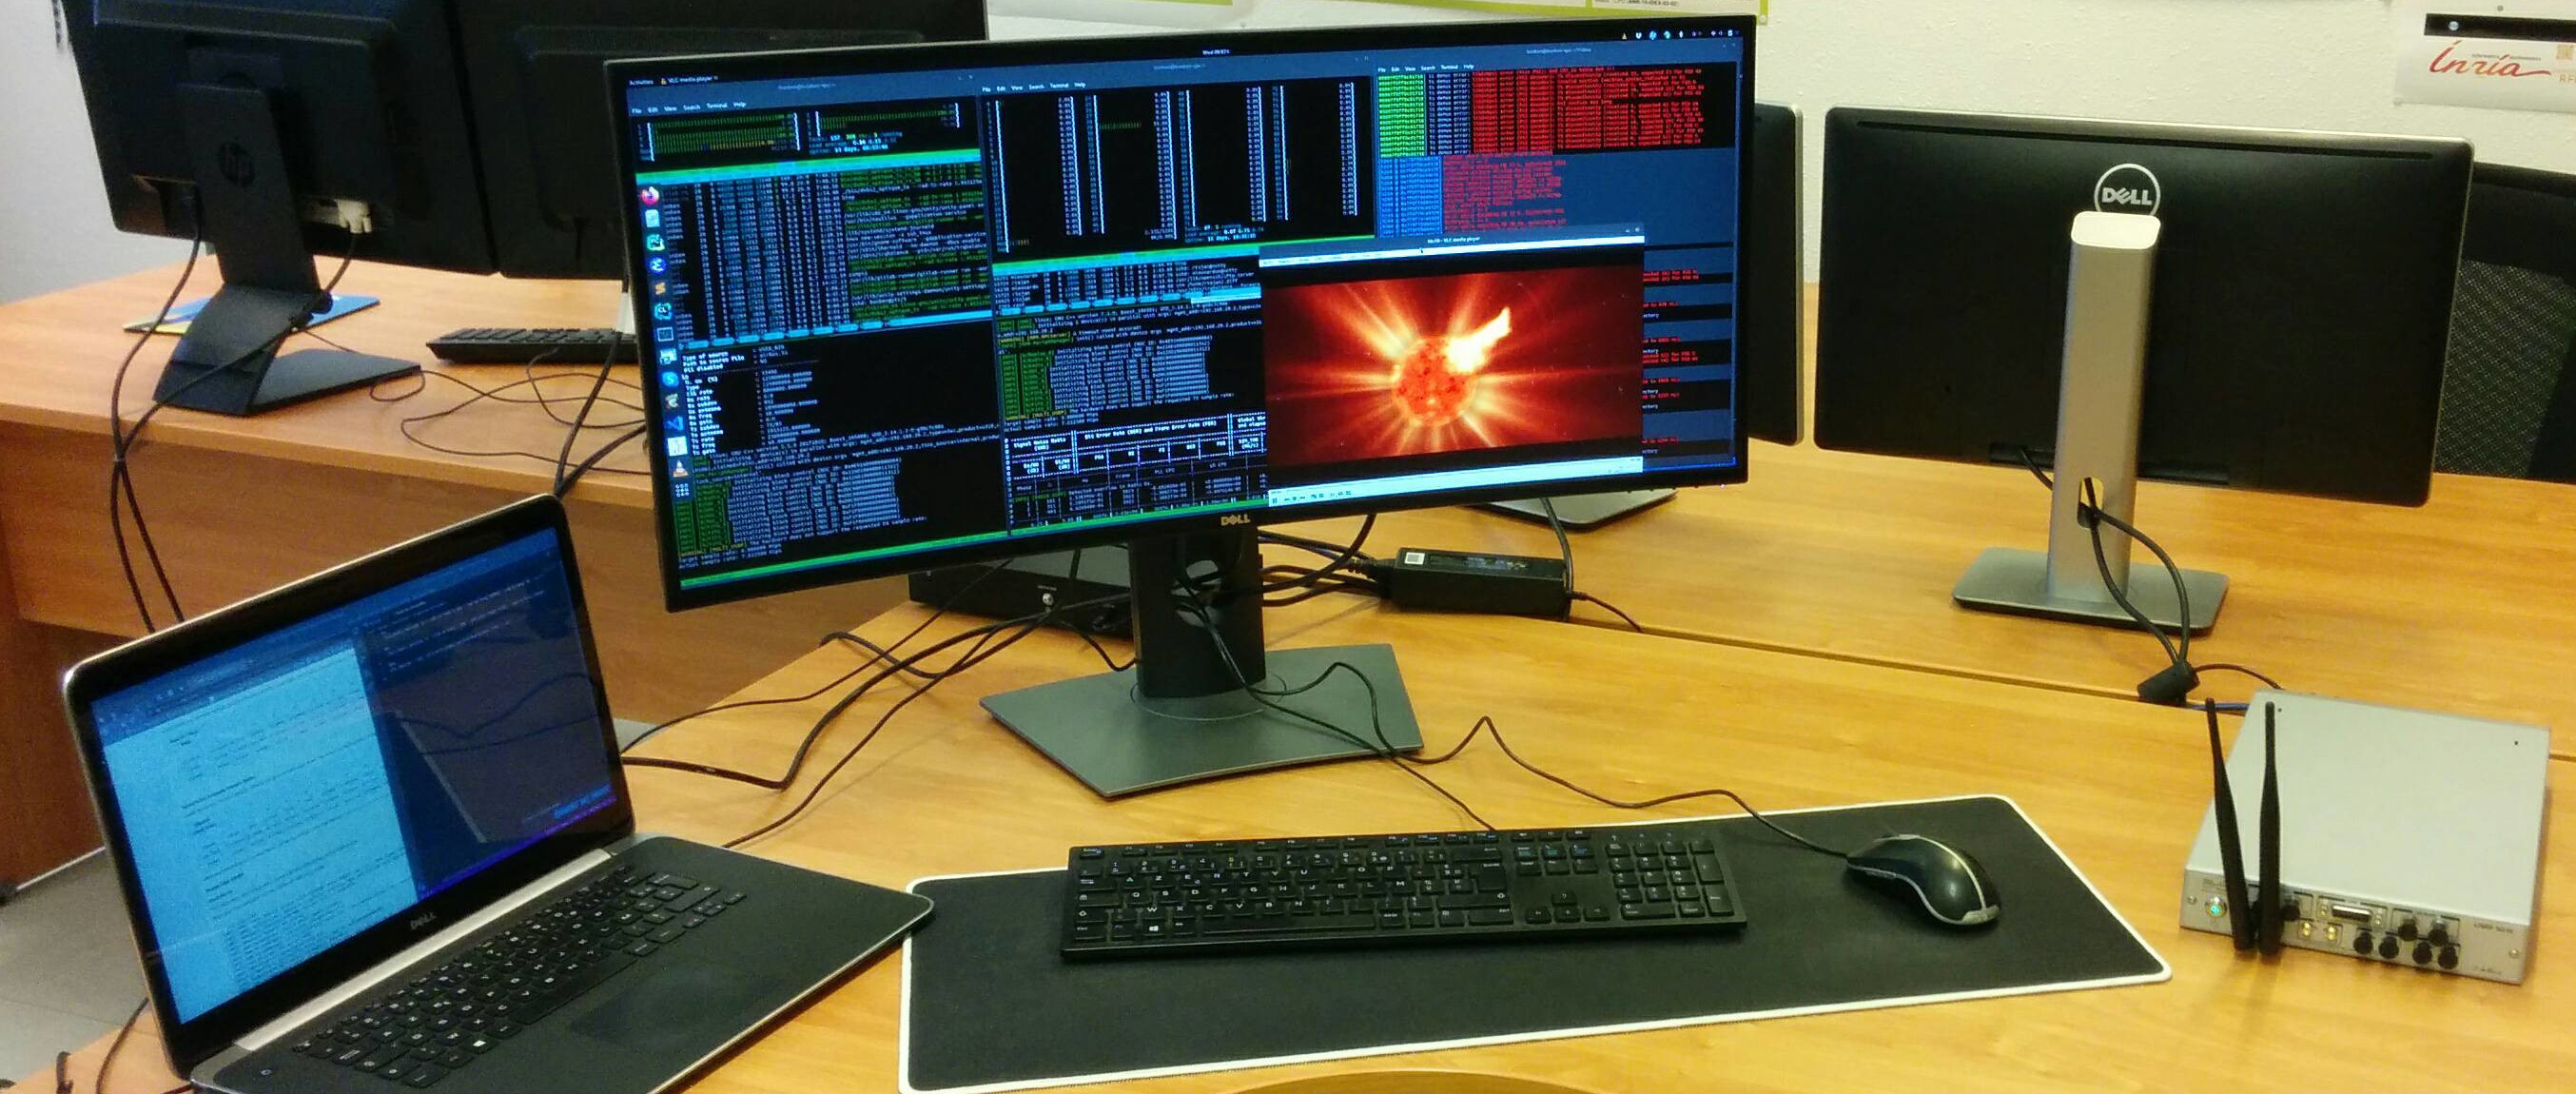
\includegraphics[scale=0.25]{pics/demo_dvbs2}
  \end{figure}
  \begin{itemize}
    \item Implement a full DVB-S2 transceiver (streaming video)
    \item Two Universal Software Radio Peripherals (USRPs) N320 for the RF
    \item One middle class computer for the transmitter (Tx) BB processing => SDR
    \item One server class computer for the receiver (Rx) BB processing => SDR
  \end{itemize}
  \vfill
  \begin{table}[htp]
    \centering
    \resizebox{1.0\linewidth}{!}{
    % \begin{tabular}{c c c c c c c c}
    %   \textbf{Config.} & \textbf{Modulation} & \textbf{Rate} $\bm{R}$ & $\bm{K_\text{\textbf{BCH}}}$ & $\bm{K_\text{\textbf{LDPC}}}$ & $\bm{N_\text{\textbf{LDPC}}}$ & $\bm{N_\text{\textbf{PLH}}}$ & \textbf{Interleaver}\\
    %   \hline \hline
    %   MODCOD 1 &  QPSK & 3/5 &  9552 &  9720 & 16200 & 16740 & no\\
    %   MODCOD 2 &  QPSK & 8/9 & 14232 & 14400 & 16200 & 16740 & no\\
    %   MODCOD 3 & 8-PSK & 8/9 & 14232 & 14400 & 16200 & 16740 & column/row\\
    % \end{tabular}
    \begin{tabular}{c c c c c c c}
      \textbf{Config.} & \textbf{Modulation} & \textbf{Rate} $\bm{R}$ & $\bm{K_\text{\textbf{BCH}}}$ & $\bm{K_\text{\textbf{LDPC}}}$ & $\bm{N_\text{\textbf{LDPC}}}$ & $\bm{\mathcal{T}_i}$ (Rx, Seq.)\\
      \hline \hline
      \textcolor{Paired-1}{MODCOD 1} &  QPSK & 3/5 &  9552 &  9720 & 16200 & 3.4 Mb/s\\
      \textcolor{Paired-3}{MODCOD 2} &  QPSK & 8/9 & 14232 & 14400 & 16200 & 4.1 Mb/s\\
      \textcolor{Paired-5}{MODCOD 3} & 8-PSK & 8/9 & 14232 & 14400 & 16200 & 4.0 Mb/s\\
    \end{tabular}
    }
    \caption*{Selected DVB-S2 configurations (MODCOD).}
  \end{table}
  \vfill

\end{frame}

\begin{frame}{Transmitter}
  \vfill
  \begin{figure}[!h]
    \centering
    \scalebox{.50}{
    \begin{tikzpicture}%[scale=\tikzscale]
      \tikzset{ tsk/.style ={draw=Paired-1, rounded corners=0pt, text=Paired-1, minimum height=1.0cm, minimum width=1cm} }
      \tikzset{ stsk/.style={draw=Paired-1, rounded corners=0pt, text=Paired-1, minimum height=1.0cm, minimum width=1cm, fill=Paired-1!7} }
      \tikzset{ ss/.style  ={draw=Paired-9, rounded corners=2pt, minimum height=1.5cm} }
      \tikzset{ seq/.style ={draw=Paired-11, dashed, rounded corners=2pt} }
      \tikzset{ mdl/.style ={draw=Paired-3,  dashed, rounded corners=2pt} }
      \tikzset{ pip/.style ={draw=Dark2-8,  dotted, thick, rounded corners=2pt} }
      \tikzset{ sin/.style ={draw=Paired-7, circle, minimum width=0.3cm, text=black, preaction={fill=white}, pattern=north east lines, pattern color=Paired-7} }
      \tikzset{ sout/.style={draw=Paired-5, circle, minimum width=0.3cm, text=black, preaction={fill=white}, pattern=crosshatch dots, pattern color=Paired-5} }

      \node[stsk                    , align=center] (t1) at (0.0, 2.0) {~generate~~\\($t^{\text{Tx}}_1$)};
      \node[tsk , right=2.00cm of t1, align=center] (t2)               {~scramble~~\\($t^{\text{Tx}}_2$)};
      \node[tsk , right=1.25cm of t2, align=center] (t3)               {~encode~~\\($t^{\text{Tx}}_3$)};
      \node[tsk , right=1.25cm of t3, align=center] (t4)               {~encode~~\\($t^{\text{Tx}}_4$)};
      \node[tsk , right=1.25cm of t4, align=center] (t5)               {~interleave~~\\($t^{\text{Tx}}_5$)};
      \node[tsk,  below=1.00cm of t2, align=center] (t6)               {~modulate~~\\($t^{\text{Tx}}_6$)};
      \node[tsk , right=1.25cm of t6, align=center] (t7)               {~insert~~\\($t^{\text{Tx}}_7$)};
      \node[tsk , right=1.25cm of t7, align=center] (t8)               {~scramble~~\\($t^{\text{Tx}}_8$)};
      \node[stsk, right=4.60cm of t8, align=center] (t9)               {~filter~~\\($t^{\text{Tx}}_9$)};
      \node[stsk, right=1.00cm of t9, align=center] (t10)              {~send~~\\($t^{\text{Tx}}_{10}$)};

      \node[sout, at=(t1.east) ] (t1_so)  {};
      \node[sin,  at=(t2.west) ] (t2_si)  {};
      \node[sout, at=(t2.east) ] (t2_so)  {};
      \node[sin,  at=(t3.west) ] (t3_si)  {};
      \node[sout, at=(t3.east) ] (t3_so)  {};
      \node[sin,  at=(t4.west) ] (t4_si)  {};
      \node[sout, at=(t4.east) ] (t4_so)  {};
      \node[sin,  at=(t5.west) ] (t5_si)  {};
      \node[sout, at=(t5.east) ] (t5_so)  {};
      \node[sin,  at=(t6.west) ] (t6_si)  {};
      \node[sout, at=(t6.east) ] (t6_so)  {};
      \node[sin,  at=(t7.west) ] (t7_si)  {};
      \node[sout, at=(t7.east) ] (t7_so)  {};
      \node[sin,  at=(t8.west) ] (t8_si)  {};
      \node[sout, at=(t8.east) ] (t8_so)  {};
      \node[sin,  at=(t9.west) ] (t9_si)  {};
      \node[sout, at=(t9.east) ] (t9_so)  {};
      \node[sin,  at=(t10.west)] (t10_si) {};

      \node[mdl, label={[Paired-3]above:Source Binary File},  fit=(t1)           (t1_so)] (m1) {};
      \node[mdl, label={[Paired-3]above:Scrambler Binary},    fit=(t2)  (t2_si)  (t2_so)] (m2) {};
      \node[mdl, label={[Paired-3]above:Encoder BCH},         fit=(t3)  (t3_si)  (t3_so)] (m3) {};
      \node[mdl, label={[Paired-3]above:Encoder LDPC},        fit=(t4)  (t4_si)  (t4_so)] (m4) {};
      \node[mdl, label={[Paired-3]above:Interleaver},         fit=(t5)  (t5_si)  (t5_so)] (m5) {};
      \node[mdl, label={[Paired-3]above:Modem PSK},           fit=(t6)  (t6_si)  (t6_so)] (m6) {};
      \node[mdl, label={[Paired-3]above:Framer PLH},          fit=(t7)  (t7_si)  (t7_so)] (m7) {};
      \node[mdl, label={[Paired-3]above:Scrambler Symbol},    fit=(t8)  (t8_si)  (t8_so)] (m8) {};
      \node[mdl, label={[Paired-3]above:Filter Shaping},      fit=(t9)  (t9_si)  (t9_so)] (m9) {};
      \node[mdl, label={[Paired-3]above:Radio},               fit=(t10) (t10_si)        ] (m9) {};

      \draw[->,>=latex] (t1_so) -- (t2_si)  node [midway, above] {};
      \draw[->,>=latex] (t2_so) -- (t3_si)  node [midway, above] {};
      \draw[->,>=latex] (t3_so) -- (t4_si)  node [midway, above] {};
      \draw[->,>=latex] (t4_so) -- (t5_si)  node [midway, above] {};
      \draw[->,>=latex] (t5_so) -- (13.9,2.0) -- (13.9,1.15) -- (2.25,1.15) -- (2.25,0) -- (t6_si)  node [midway, above] {};
      \draw[->,>=latex] (t6_so) -- (t7_si)  node [midway, above] {};
      \draw[->,>=latex] (t7_so) -- (t8_si)  node [midway, above] {};
      \draw[->,>=latex] (t8_so) -- (t9_si)  node [midway, above] {};
      \draw[->,>=latex] (t9_so) -- (t10_si) node [midway, above] {};
      \draw[black, -] (t10.east)--++(0:1.0cm) node[antenna, label={[above,yshift=+2.15cm]USRP}] {};

      \node[seq, minimum height=2.5cm, minimum width=3.5cm,  label={[Paired-11]below:Stage 1}, fit=(t1) (t1_so)                                      ] (seq1) {};
      \node[seq, minimum height=4.5cm, minimum width=12.0cm, label={[Paired-11]below:Stage 2}, fit=(t2_si) (t2) (t3) (t4) (t5) (t6) (t7) (t8) (t8_so)] (seq2) {};
      \node[seq, minimum height=2.5cm, minimum width=4.5cm,  label={[Paired-11]below:Stage 3}, fit=(t9_si) (t10)                                     ] (seq3) {};
    \end{tikzpicture}
    }
  \end{figure}
  \vfill
\end{frame}

\begin{frame}{Receiver}
  \vspace{-0.3cm}
  \begin{figure}[!h]
    \centering
    \scalebox{.40}{
    \begin{tikzpicture}%[scale=\tikzscale]
      \tikzset{ tsk/.style ={draw=Paired-1, rounded corners=0pt, text=Paired-1, minimum height=1.0cm, minimum width=1cm} }
      \tikzset{ stsk/.style={draw=Paired-1, rounded corners=0pt, text=Paired-1, minimum height=1.0cm, minimum width=1cm, fill=Paired-1!7} }
      \tikzset{ ss/.style  ={draw=Paired-9, rounded corners=2pt, minimum height=1.5cm} }
      \tikzset{ seq/.style ={draw=Paired-11, dashed, rounded corners=2pt} }
      \tikzset{ mdl/.style ={draw=Paired-3,  dashed, rounded corners=2pt} }
      \tikzset{ pip/.style ={draw=Dark2-8,  dotted, thick, rounded corners=2pt} }
      \tikzset{ sin/.style ={draw=Paired-7, circle, minimum width=0.3cm, text=black, preaction={fill=white}, pattern=north east lines, pattern color=Paired-7} }
      \tikzset{ sout/.style={draw=Paired-5, circle, minimum width=0.3cm, text=black, preaction={fill=white}, pattern=crosshatch dots, pattern color=Paired-5} }

      \node[stsk                     , align=center] (t1) at ( 0.0, 2.0) {~receive~~\\($t^{\text{Rx}}_1$)};
      \node[tsk , right=2.00cm of t1 , align=center] (t2)                {~imultiply~~\\($t^{\text{Rx}}_2$)};
      \node[stsk, right=1.00cm of t2 , align=center] (t3)                {~synchronize~~\\($t^{\text{Rx}}_3$)};
      \node[stsk, right=1.00cm of t3 , align=center] (t4)                {~filter~~\\($t^{\text{Rx}}_4$)};
      \node[stsk, below=3.50cm of t2 , align=center] (t5)                {~synchronize~~\\($t^{\text{Rx}}_5$)};
      \node[stsk, right=2.00cm of t5 , align=center] (t6)                {~extract~~\\($t^{\text{Rx}}_6$)};
      \node[tsk , right=1.00cm of t6 , align=center] (t7)                {~imultiply~~\\($t^{\text{Rx}}_7$)};
      \node[stsk, right=1.00cm of t7 , align=center] (t8)                {~synchronize~~\\($t^{\text{Rx}}_8$)};
      \node[tsk , below=3.50cm of t5 , align=center] (t9)                {~descramble~~\\($t^{\text{Rx}}_9$)};
      \node[stsk, right=1.00cm of t9 , align=center] (t10)               {~synchronize~~\\($t^{\text{Rx}}_{10}$)};
      \node[tsk , right=1.00cm of t10, align=center] (t11)               {~synchronize~~\\($t^{\text{Rx}}_{11}$)};
      \node[tsk , right=3.00cm of t11, align=center] (t12)               {~remove~~\\($t^{\text{Rx}}_{12}$)};
      \node[tsk , right=1.00cm of t12, align=center] (t13)               {~estimate~~\\($t^{\text{Rx}}_{13}$)};
      \node[tsk , below=3.50cm of t9 , align=center] (t14)               {~demodulate~~\\($t^{\text{Rx}}_{14}$)};
      \node[tsk , right=1.00cm of t14, align=center] (t15)               {~deinterleave~~\\($t^{\text{Rx}}_{15}$)};
      \node[tsk , right=1.00cm of t15, align=center] (t16)               {~decode SIHO~~\\($t^{\text{Rx}}_{16}$)};
      \node[tsk , right=1.00cm of t16, align=center] (t17)               {~decode HIHO~~\\($t^{\text{Rx}}_{17}$)};
      \node[tsk , right=1.00cm of t17, align=center] (t18)               {~descramble~~\\($t^{\text{Rx}}_{18}$)};
      \node[stsk, right=2.00cm of t18, align=center] (t19)               {~send~~\\($t^{\text{Rx}}_{19}$)};

      \node[sout, at=(t1.east)                ] (t1_so)  {};
      \node[sin,  at=(t2.west)                ] (t2_si)  {};
      \node[sout, at=(t2.east)                ] (t2_so)  {};
      \node[sin,  at=(t3.west)                ] (t3_si)  {};
      \node[sout, at=(t3.east)                ] (t3_so)  {};
      \node[sin,  at=(t4.west)                ] (t4_si)  {};
      \node[sout, at=(t4.east)                ] (t4_so)  {};
      \node[sin,  at=(t5.west)                ] (t5_si)  {};
      \node[sout, at=(t5.east), yshift=+0.25cm] (t5_so1) {};
      \node[sout, at=(t5.east), yshift=-0.25cm] (t5_so2) {};
      \node[sin,  at=(t6.west), yshift=+0.25cm] (t6_si1) {};
      \node[sin,  at=(t6.west), yshift=-0.25cm] (t6_si2) {};
      \node[sout, at=(t6.east)                ] (t6_so)  {};
      \node[sin,  at=(t7.west)                ] (t7_si)  {};
      \node[sout, at=(t7.east)                ] (t7_so)  {};
      \node[sin,  at=(t8.west)                ] (t8_si)  {};
      \node[sout, at=(t8.east), yshift=+0.25cm] (t8_so1) {};
      \node[sout, at=(t8.east), yshift=-0.25cm] (t8_so2) {};
      \node[sin,  at=(t9.west)                ] (t9_si)  {};
      \node[sout, at=(t9.east)                ] (t9_so)  {};
      \node[sin,  at=(t10.west)               ] (t10_si) {};
      \node[sout, at=(t10.east)               ] (t10_so) {};
      \node[sin,  at=(t11.west)               ] (t11_si) {};
      \node[sout, at=(t11.east)               ] (t11_so) {};
      \node[sin,  at=(t12.west)               ] (t12_si) {};
      \node[sout, at=(t12.east)               ] (t12_so) {};
      \node[sin,  at=(t13.west)               ] (t13_si) {};
      \node[sout, at=(t13.east)               ] (t13_so) {};
      \node[sin,  at=(t14.west)               ] (t14_si) {};
      \node[sout, at=(t14.east)               ] (t14_so) {};
      \node[sin,  at=(t15.west)               ] (t15_si) {};
      \node[sout, at=(t15.east)               ] (t15_so) {};
      \node[sin,  at=(t16.west)               ] (t16_si) {};
      \node[sout, at=(t16.east)               ] (t16_so) {};
      \node[sin,  at=(t17.west)               ] (t17_si) {};
      \node[sout, at=(t17.east)               ] (t17_so) {};
      \node[sin,  at=(t18.west)               ] (t18_si) {};
      \node[sout, at=(t18.east)               ] (t18_so) {};
      \node[sin,  at=(t19.west)               ] (t19_si) {};

      \draw[black, -] (t1.west)--++(0:-1.0cm) node[antenna, label={[above,yshift=+2.15cm]USRP}] {};
      \draw[->,>=latex] (t1_so) -- (t2_si)  node [midway, above] {};
      \draw[->,>=latex] (t2_so) -- (t3_si)  node [midway, above] {};
      \draw[->,>=latex] (t3_so) -- (t4_si)  node [midway, above] {};
      % \draw[->,>=latex] (t4_so) -- (t5_si)  node [midway, above] {};
      \draw[->,>=latex] (t4_so) -| (11.0,-0.5) -- (1.5,-0.5) |- (t5_si)  node [midway, above] {};
      \draw[->,>=latex] (t5_so1) -- (t6_si1)  node [midway, above] {};
      \draw[->,>=latex] (t5_so2) -- (t6_si2)  node [midway, above] {};
      % \draw[->,>=latex] (t5_so) -- (13.9,2.0) -- (13.9,1.15) -- (2.25,1.15) -- (2.25,0) -- (t6_si)  node [midway, above] {};
      \draw[->,>=latex] (t6_so) -- (t7_si)  node [midway, above] {};
      \draw[->,>=latex] (t7_so) -- (t8_si)  node [midway, above] {};
      % \draw[->,>=latex] (t8_so) -- (t9_si)  node [midway, above] {};
      \draw[->,>=latex] (t8_so1) -| (15.5,-5.0) -- (1.5,-5.0) |- (t9_si)  node [midway, above] {};
      \draw[->,>=latex] (t9_so) -- (t10_si) node [midway, above] {};
      \draw[->,>=latex] (t10_so) -- (t11_si) node [midway, above] {};
      \draw[->,>=latex] (t11_so) -- (t12_si) node [midway, above] {};
      \draw[->,>=latex] (t12_so) -- (t13_si) node [midway, above] {};
      % \draw[->,>=latex] (t13_so) -- (t14_si) node [midway, above] {};
      \draw[->,>=latex] (t13_so) -| (19.5,-9.5) -- (1.5,-9.5) |- (t14_si)  node [midway, above] {};

      \draw[->,>=latex] (t14_so) -- (t15_si) node [midway, above] {};
      \draw[->,>=latex] (t15_so) -- (t16_si) node [midway, above] {};
      \draw[->,>=latex] (t16_so) -- (t17_si) node [midway, above] {};
      \draw[->,>=latex] (t17_so) -- (t18_si) node [midway, above] {};
      \draw[->,>=latex] (t18_so) -- (t19_si) node [midway, above] {};

      \node[seq, minimum height=3.5cm, minimum width=3.2cm,   label={[Paired-11]below:Stage 1}, fit=(t1)  (t1_so)                                                          ] (seq1) {};
      \node[seq, minimum height=3.5cm, minimum width=8.5cm,   label={[Paired-11]below:Stage 2}, fit=(t2)  (t2_si)  (t2_so)  (t3)  (t3_si)  (t3_so)  (t4)  (t4_si)  (t4_so) ] (seq2) {};
      \node[seq, minimum height=3.5cm, minimum width=3.5cm,   label={[Paired-11]below:Stage 3}, fit=(t5)  (t5_si)  (t5_so1)                                                ] (seq3) {};
      \node[seq, minimum height=3.5cm, minimum width=9.0cm,   label={[Paired-11]below:Stage 4}, fit=(t6)  (t6_si1) (t6_so)  (t7)  (t7_si)  (t7_so)  (t8)  (t8_si)  (t8_so1)] (seq4) {};
      \node[seq, minimum height=3.5cm, minimum width=10.0cm,  label={[Paired-11]below:Stage 5}, fit=(t9)  (t9_si)  (t9_so)  (t10) (t10_si) (t10_so) (t11) (t11_si) (t11_so)] (seq5) {};
      \node[seq, minimum height=3.5cm, minimum width=6.5cm,   label={[Paired-11]below:Stage 6}, fit=(t12) (t12_si) (t12_so) (t13) (t13_si) (t13_so)                        ] (seq6) {};
      \node[seq, minimum height=3.5cm, minimum width=17.0cm,  label={[Paired-11]below:Stage 7}, fit=(t14_si) (t18_so)                                                      ] (seq7) {};
      \node[seq, minimum height=3.5cm, minimum width=3.2cm,   label={[Paired-11]below:Stage 8}, fit=(t19_si) (t19)                                                         ] (seq8) {};

      \node[mdl, label={[Paired-3, align=center]above:Radio},                          fit=(t1)           (t1_so)     ] (m1)  {};
      \node[mdl, label={[Paired-3, align=center]above:Multiplier AGC},                 fit=(t2)  (t2_si)  (t2_so)     ] (m2)  {};
      \node[mdl, label={[Paired-3, align=center]above:Synchronizer\\Freq. Coarse},     fit=(t3)  (t3_si)  (t3_so)     ] (m3)  {};
      \node[mdl, label={[Paired-3, align=center]above:Filter\\Matched},                fit=(t4)  (t4_si)  (t4_so)     ] (m4)  {};
      \node[mdl, label={[Paired-3, align=center]above:Synchronizer Timing\\(Gardner)}, fit=(t5)  (t5_si)  (t6) (t6_so)] (m5)  {};
      \node[mdl, label={[Paired-3, align=center]above:Multiplier AGC},                 fit=(t7)  (t7_si)  (t7_so)     ] (m6)  {};
      \node[mdl, label={[Paired-3, align=center]above:Synchronizer\\Frame},            fit=(t8)  (t8_si)  (t8_so1)    ] (m7)  {};
      \node[mdl, label={[Paired-3, align=center]above:Scrambler Symbol},               fit=(t9)  (t9_si)  (t9_so)     ] (m8)  {};
      \node[mdl, label={[Paired-3, align=center]above:Synchronizer\\Freq. Fine L\&R},  fit=(t10) (t10_si) (t10_so)    ] (m9)  {};
      \node[mdl, label={[Paired-3, align=center]above:Synchronizer\\Freq. Fine P/F},   fit=(t11) (t11_si) (t11_so)    ] (m10) {};
      \node[mdl, label={[Paired-3, align=center]above:Framer PLH},                     fit=(t12) (t12_si) (t12_so)    ] (m11) {};
      \node[mdl, label={[Paired-3, align=center]above:Noise Estimator},                fit=(t13) (t13_si) (t13_so)    ] (m12) {};
      \node[mdl, label={[Paired-3, align=center]above:Modem PSK},                      fit=(t14) (t14_si) (t14_so)    ] (m13) {};
      \node[mdl, label={[Paired-3, align=center]above:Interleaver},                    fit=(t15) (t15_si) (t15_so)    ] (m14) {};
      \node[mdl, label={[Paired-3, align=center]above:Decoder LDPC},                   fit=(t16) (t16_si) (t16_so)    ] (m15) {};
      \node[mdl, label={[Paired-3, align=center]above:Decoder BCH},                    fit=(t17) (t17_si) (t17_so)    ] (m16) {};
      \node[mdl, label={[Paired-3, align=center]above:Scrambler Binary},               fit=(t18) (t18_si) (t18_so)    ] (m17) {};
      \node[mdl, label={[Paired-3, align=center]above:Sink Binary File},               fit=(t19) (t19_si)             ] (m18) {};


      % \draw[-,>=latex, very thick] (12.55,-6.0) -- (12.55,-8) node [midway, above] {};
      % \draw[-,>=latex, very thick] (12.65,-6.0) -- (12.65,-8) node [midway, above] {};
      % \draw[-,>=latex, very thick] (14.55,2.0) -- (14.55,1.5) node [midway, above] {};
      % \draw[-,>=latex, very thick] (14.65,2.0) -- (14.65,1.5) node [midway, above] {};
      % \node at (17.00,1.75) {End of the learning phase 3};
    \end{tikzpicture}
    }
  \end{figure}
\end{frame}

\begin{frame}{Evaluations}
  \vspace{-0.2cm}
  \begin{figure}[!h]
    \centering
    \scalebox{.40}{
    \begin{tikzpicture}%[scale=\tikzscale]
    \begin{groupplot}[/pgfplots/table/ignore chars={|}, %footnotesize,
                      height=0.77\textwidth, width=1.0\textwidth,
                      xticklabel style={black!70}, yticklabel style={black!70},
                      group style={group name=scl_2048, group size= 2 by 1, horizontal sep=2cm, vertical sep=2.0cm},
                      ymode = log,
                      % ymin=0.000000001, ymax=0.05,
                      % xmin=0, xmax=2,
                      % xtick={0,0.5,...,4.5},
                      xlabel=$E_b/N_0~\text{(dB)}$,
                      grid=both, grid style={gray!30},
                      %tick align=outside, tickpos=left,
                      legend pos=north east]
      \nextgroupplot[ylabel=BER]

      \addplot[mark=square,    Paired-1,    semithick, dashed, mark options={solid}] table [x=Eb/N0, y=BER] {../main/chapter5/fig/dvbs2/bfer/dat/data_QPSK_R_3_5_BB.txt};  \label{plot:llline1}
      \addplot[mark=triangle,  Paired-1!80, semithick, dashed, mark options={solid}] table [x=Eb/N0, y=BER] {../main/chapter5/fig/dvbs2/bfer/dat/data_QPSK_R_3_5_sim.txt}; \label{plot:llline2}
      \addplot[mark=o,         Paired-1!60, semithick, dashed, mark options={solid}, domain=0:0.2, error bars/.cd, x dir=both,x fixed=0.2, y dir=both,y explicit, error bar style={solid}] table [x=Eb/N0, y=BER] {../main/chapter5/fig/dvbs2/bfer/dat/data_QPSK_R_3_5_rad.txt}; \label{plot:llline3}

      \addplot[mark=square,    Paired-3,    semithick, dotted, mark options={solid}] table [x=Eb/N0, y=BER] {../main/chapter5/fig/dvbs2/bfer/dat/data_QPSK_R_8_9_BB.txt};  \label{plot:llline4}
      \addplot[mark=triangle,  Paired-3!80, semithick, dotted, mark options={solid}] table [x=Eb/N0, y=BER] {../main/chapter5/fig/dvbs2/bfer/dat/data_QPSK_R_8_9_sim.txt}; \label{plot:llline5}
      \addplot[mark=o,         Paired-3!60, semithick, dotted, mark options={solid}, domain=0:0.2, error bars/.cd, x dir=both,x fixed=0.2, y dir=both,y explicit, error bar style={solid}] table [x=Eb/N0, y=BER] {../main/chapter5/fig/dvbs2/bfer/dat/data_QPSK_R_8_9_rad.txt}; \label{plot:llline6}

      \addplot[mark=square,    Paired-5,    semithick,         mark options={solid}] table [x=Eb/N0, y=BER] {../main/chapter5/fig/dvbs2/bfer/dat/data_8PSK_R_8_9_BB.txt};  \label{plot:llline7}
      \addplot[mark=triangle,  Paired-5!80, semithick,         mark options={solid}] table [x=Eb/N0, y=BER] {../main/chapter5/fig/dvbs2/bfer/dat/data_8PSK_R_8_9_sim.txt}; \label{plot:llline8}
      \addplot[mark=o,         Paired-5!60, semithick,         mark options={solid}, domain=0:0.2, error bars/.cd, x dir=both,x fixed=0.2, y dir=both,y explicit, error bar style={solid}] table [x=Eb/N0, y=BER] {../main/chapter5/fig/dvbs2/bfer/dat/data_8PSK_R_8_9_rad.txt}; \label{plot:llline9}

      \coordinate (legend) at (axis description cs:1.375,1.05);

      \nextgroupplot[ylabel=FER]

      \addplot[mark=square,    Paired-1,    semithick, dashed, mark options={solid}] table [x=Eb/N0, y=FER] {../main/chapter5/fig/dvbs2/bfer/dat/data_QPSK_R_3_5_BB.txt};  \label{plot:llline1}
      \addplot[mark=triangle,  Paired-1!80, semithick, dashed, mark options={solid}] table [x=Eb/N0, y=FER] {../main/chapter5/fig/dvbs2/bfer/dat/data_QPSK_R_3_5_sim.txt}; \label{plot:llline2}
      \addplot[mark=o,         Paired-1!60, semithick, dashed, mark options={solid}, domain=0:0.2, error bars/.cd, x dir=both,x fixed=0.2, y dir=both,y explicit, error bar style={solid}] table [x=Eb/N0, y=FER] {../main/chapter5/fig/dvbs2/bfer/dat/data_QPSK_R_3_5_rad.txt}; \label{plot:llline3}

      \addplot[mark=square,    Paired-3,    semithick, dotted, mark options={solid}] table [x=Eb/N0, y=FER] {../main/chapter5/fig/dvbs2/bfer/dat/data_QPSK_R_8_9_BB.txt};  \label{plot:llline4}
      \addplot[mark=triangle,  Paired-3!80, semithick, dotted, mark options={solid}] table [x=Eb/N0, y=FER] {../main/chapter5/fig/dvbs2/bfer/dat/data_QPSK_R_8_9_sim.txt}; \label{plot:llline5}
      \addplot[mark=o,         Paired-3!60, semithick, dotted, mark options={solid}, domain=0:0.2, error bars/.cd, x dir=both,x fixed=0.2, y dir=both,y explicit, error bar style={solid}] table [x=Eb/N0, y=FER] {../main/chapter5/fig/dvbs2/bfer/dat/data_QPSK_R_8_9_rad.txt}; \label{plot:llline6}

      \addplot[mark=square,    Paired-5,    semithick,         mark options={solid}] table [x=Eb/N0, y=FER] {../main/chapter5/fig/dvbs2/bfer/dat/data_8PSK_R_8_9_BB.txt};  \label{plot:llline7}
      \addplot[mark=triangle,  Paired-5!80, semithick,         mark options={solid}] table [x=Eb/N0, y=FER] {../main/chapter5/fig/dvbs2/bfer/dat/data_8PSK_R_8_9_sim.txt}; \label{plot:llline8}
      \addplot[mark=o,         Paired-5!60, semithick,         mark options={solid}, domain=0:0.2, error bars/.cd, x dir=both,x fixed=0.2, y dir=both,y explicit, error bar style={solid}] table [x=Eb/N0, y=FER] {../main/chapter5/fig/dvbs2/bfer/dat/data_8PSK_R_8_9_rad.txt}; \label{plot:llline9}
    \end{groupplot}

    \matrix [
        draw,
        matrix of nodes,
        anchor=south east,
        fill=white,
        ampersand replacement=\&
    ] at (legend) {
                 \& \textcolor{Paired-1}{MODCOD1} \& \textcolor{Paired-3}{MODCOD2} \& \textcolor{Paired-5}{MODCOD3} \\
        AWGN     \& \ref{plot:llline1} \& \ref{plot:llline4} \& \ref{plot:llline7} \\
        AWGN$^+$ \& \ref{plot:llline2} \& \ref{plot:llline5} \& \ref{plot:llline8} \\
        Real     \& \ref{plot:llline3} \& \ref{plot:llline6} \& \ref{plot:llline9} \\
    };
    \end{tikzpicture}
    }
  \end{figure}


% Decoding Performance

% Achieved Throughputs

  \begin{table}[htp]
    \centering
    % \caption
    %   [Throughput performance depending of the selected DVB-S2 configuration.]
    %   {Throughput performance depending of the selected DVB-S2 configuration.}
    % \label{tab:sdr_dvbs2_thr_modcod}
    {\small\resizebox{.5\linewidth}{!}{
    \begin{tabular}{c | c c | c c}
      \multirow{3}{*}{\textbf{Config.}} & \multicolumn{4}{c }{\textbf{Throughput} (Mb/s)} \\
                                        & \multicolumn{2}{c |}{\textbf{Sequential}} & \multicolumn{2}{c }{\textbf{Parallel}} \\
                                        & \textbf{Info.} & \textbf{Coded} & \textbf{Info.} & \textbf{Coded} \\
      \hline \hline
      \textcolor{Paired-1}{MODCOD 1} &  3.4 & 5.7 & 37 & 62 \\
      \textcolor{Paired-3}{MODCOD 2} &  4.1 & 4.6 & 55 & 62 \\
      \textcolor{Paired-5}{MODCOD 3} &  4.0 & 4.5 & 80 & 90 \\
    \end{tabular}
    }}
  \end{table}

\end{frame}

%!TEX root = ../my_thesis.tex

\graphicspath{{main/conclusion/fig/}}

\chapter*{Conclusions and Perspectives}
\markboth{Conclusions and Perspectives}{Conclusions and Perspectives}
\addcontentsline{toc}{chapter}{Conclusions and Perspectives}

\section*{Conclusion}

In the context of digital communications, channel coding schemes are widely
spread. This thesis focuses on three channel codes that are present in most of
the current digital communication standards: the LDPC codes, the polar codes and
the turbo codes. In digital communication systems, most of the computational
time is spent in the receiver and more precisely in the decoding stage. This is
why, we propose efficient implementations of these decoding algorithms on CPUs.
The proposed implementations enable fast evaluations and validations of various
configurations. Moreover, there is a growing need to build full digital
communication chains in software. This is what we call the Software-Defined
Radio (SDR). Thus, the challenge is to take advantage of multi-core CPU
architectures to schedule the processing in parallel.

Several optimization strategies have been presented and discussed. One of the
main characteristic of the digital communication algorithms is that they have a
very short execution time (low latency). Thus, the most adapted parallelism
level presents in the actual CPUs is the Single Instruction Multiple Data (SIMD)
model. In Section~\ref{sec:opt_mipp}, \MIPP, a generic SIMD library, is
proposed. This library enables simplified and portable use of the CPUs
vectorized instructions. Then, in Section~\ref{sec:opt_vec}, two main
vectorization strategies are detailed: the intra-frame SIMD strategy that
enables very low latency implementations and the inter-frame SIMD strategy that
enables very high throughput implementations. The intra-frame SIMD strategy
consists in using the algorithm inherent parallelism to speedup the computation
in a single frame while the inter-frame SIMD strategy processes several frames
in parallel. In a second part of this chapter, specific optimizations for each
channel codes are given. First, a new SIMD implementation of the LDPC Belief
Propagation (BP) decoder is proposed. This decoder rests upon the inter-frame
strategy and focuses on maximizing the flexibility. Indeed, it is able to adapt
to many algorithmic sub-variants which is without precedent in the domain. Then,
the optimizations of two polar decoders are proposed, namely the Successive
Cancellation (SC) and the Successive Cancellation List (SCL) algorithms. Both
the inter-frame and intra-frame strategies are implemented. This two decoders
are based on a recursive description and the decoding process can be seen as a
tree traversal. Some specific optimizations like the tree pruning are performed
to drastically reduce the number of tree nodes. The recursive calls have also
been unrolled and generated decoders are proposed to reach the best possible
throughputs and latencies. This comes at the cost of reduced flexibility.
Finally, an SIMD implementation of the turbo decoder (max-log-MAP algorithms) is
given. The implementation uses the inter-frame SIMD strategy and targets high
throughputs. Specific optimizations have been made to increase the decoder
efficiency: some loops at the core of the decoding process have been merged and
unrolled to increase the registers reuse.

\AFFECT is a library of digital communication algorithms, developed as part of
this thesis, focusing on high performance implementations. Its software
architecture supports the algorithmic heterogeneity. Many channel codes are
supported like the LDPC codes, the polar codes and the turbo codes detailed
before. To the best of our knowledge, \AFFECT is the library with the most
comprehensive support for channel coding algorithms. The toolbox also includes a
BER/FER simulator. Many digital communication systems can be evaluated over
various parameters. The simulator takes advantage of the multi-core CPU
architectures to reduce the restitution time. All these features have been
designed to enable reproducible science. A BER/FER comparator tool has been
developed to easily search in a database of 500 pre-simulated BER/FER
references. All there references are results simulated with \AFFECT and can be
reproduced. To this purpose, a pipeline of tests has been implemented. Each time
there is a modification in the source code, the database of references is
replayed to avoid regressions.

The new implementations have been evaluated and compared with the
state-of-the-art. The results show levels of performance close to the best
software implementations in the literature. Exhaustive surveys are given through
software decoder Hall of Fames (HoFs). The proposed decoders are reported as
well as state-of-the-art works. These HoFs enable to compare CPU and GPU
implementations. Some metrics like the normalized throughput, the Throughput
Under Normalized Decoding Cost (TNDC) and the energy consumption are defined.
Finally the \AFFECT simulator performance is evaluated over several server-class
CPUs. It shows that the simulator is able to take advantage of various SIMD
instructions and multi-core architectures. During the simulation of a polar
code, a peak performance of 11 Gb/s is reached on a AMD\R EPYC CPU. To the best
of our knowledge, this is the first work to reach this level of performance.

The \AFFECT library has been enriched with a new embedded Domain Specific
Language (eDSL). The main components have been designed to satisfy the SDR needs
in terms of 1) expressiveness; 2) performance. Most of the digital communication
systems can be represented by a directed graph of processing tasks (dataflow
model). The proposed eDSL uses this representation to improve the
expressiveness. Indeed, the tasks data transfers and their execution are
automatically managed by the eDSL. Moreover, the performance is an critical
aspect. To reduce the execution time, some data independent parts of the graph
of tasks can be duplicated. Each duplication can be executed on separated CPU
cores. This strategy leads to an increased throughput. However, when it cannot
be applied the well-known pipeline strategy have been implemented. Thus, the
performance of the overall communication system can be increased up to the
throughput of the slowest task. Then, the proposed eDSL is evaluated in an
applicative context: the software implementation of the DVB-S2 standard physical
layer. The results demonstrate the efficiency of the \AFFECT eDSL. Indeed, the
proposed solution matches satellite real-time constraints (30 $\thicksim$
50~Mb/s). This is the consequence of two main factors: 1) the task level
optimizations, 2) the low overhead eDSL, with among others, an efficient
implementation of the pipeline technique.

\AFFECT is currently used in several industrial contexts for simulation purposes
(Turbo concept, Airbus, Thales, Huawei) and for specific developments (CNES,
Schlumberger, Airbus, Thales, Orange, Safran), as well as in academic projects
(NAND French National Agency project, IdEx CPU, R\&T CNES). The MIT license
chosen for the project enables industrial and academic partners to reuse parts
of \AFFECT in their own projects without any restriction. Moreover, \AFFECT has
been cited in scientific publications. Many works are exploiting the \AFFECT
simulator as a reference for the decoding performance. In other works, \AFFECT
has been enriched to support new features. And, in some cases, \AFFECT is used
as a library where some sub-parts of the toolbox are reused or some
methodologies are extracted.

To conclude on this thesis work, the main contributions are 1) the definition of
task level optimization techniques that enable high performance portable
implementations of signal processing algorithms on CPUs, 2) an open-source
software that enables homogeneous uses of various algorithms and implementations
and 3) a new language dedicated to the SDR needs that enables to define digital
communication systems taking advantage of the CPUs parallel architecture.
\AFFECT has been designed for high performance keeping in mind that the
algorithms come from the signal community experts that are not familiar with CPU
optimization techniques. Consequently, there is a clear separation of concerns
between the tasks design and their parallel execution. Co-design is then
possible: signal experts can focus on the tasks description while HPC experts
can work independently on the parallel execution thanks to the eDSL abstraction.
To the best of our knowledge, \AFFECT is the first environment to propose this
level of performance combined with the integration of many digital communication
algorithms.

\section*{Perspectives}

Several study and research perspectives remain to be explored following this
thesis work. A non-exhaustive list of these perspectives is given below. This
list is given in ascending order of presupposed complexity.

First, thanks to the flexibility of the proposed software architecture, new
coding schemes can be explored. The channel coding theory is constantly evolving
and it is mandatory to be able to evaluate the performance of new schemes. For
instance, the polar codes are one of the main interest in the domain. They have
been recently generalized from their discovery by \Arikan. It is possible to
build new codes from various kernels that are not just powers of two. This is
called multi-kernel polar codes. Some preliminary works have been conducted to
find kernels that have good factorization properties. However, this is a brute
force exploration and the complexity grows exponentially with the size of the
kernels. It could be interesting to reduce the kernel exploration domain and to
apply HPC techniques to reduce the finding time. The multi-kernel polar codes
construction is a promising area of research that could lead to better
finite-length decoding performance.

One of the main contribution of this thesis is to propose efficient digital
signal processing methods and implementations on CPU. Nowadays there is a
growing interest for GPUs in the HPC community. The GPUs are very parallel
architectures. In some conditions, the GPU implementations can lead to
non-negligible reduction of the computational time compared to the
implementations on CPU. It could be interesting to study the integration of
GPU tasks in \AFFECT. One of the main challenges is to manage the CPU to GPU and
GPU to CPU transfers. On GPUs, many works are focusing on implementing only the
most compute intensive task (namely the channel decoder) or a fixed
configuration of tasks (BPSK modulation, AWGN channel and a specific coding
scheme)~\cite{Wu2011,Xianjun2013,LeGal2014a,Lai2016,Giard2016b,Keskin2017b}. The
several configurations available in \AFFECT combined with the ability to execute
tasks on both CPU and GPU would be a major improvement. Even if the GPUs are a
good alternative to the CPUs, we believe that they will not be integrated in
cloud-RAN architectures. The FPGAs look like to provide a better compromize
between power efficiency and computational performance for scaling up. Their
integration in \AFFECT could be a great challenge.

Finally, the proposed eDSL could be enriched. For instance, the pipeline stages
are given by the user while they could be found automatically. The execution
time of the tasks is mostly constant for a given CPU. Thus, an auto-tuning phase
could be applied to determine a good configuration of the pipeline stages
automatically. Moreover, the scheduling of the tasks inside a sequence is very
basic. The tasks are not executed in parallel even if the data dependencies
allow it. We think that a dynamic scheduling strategy like it can be found in
the HPC runtime libraries (see OpenMP or StarPU) would be overkill. The overhead
of a dynamic scheduler is not negligible because the execution time of the
signal processing tasks in very short (ranging from some nanoseconds to some
microseconds). However, an improved static scheduling strategy that enables
parallel executions inside sequences would certainly help to reduce the
restitution time. These improvements could lead to an extension of the \AFFECT
eDSL. Indeed, the targeted domain could be expended to the generalized streaming
applications (image/video processing, cryptographic processing, networking, DSP,
etc.). The challenge will be to identify the required additional modules and to
integrate them into the eDSL with no impact on the execution efficiency.


\appendix

\AtBeginSection[]{}
\AtBeginSubsection[]{}

\section[References]{References}

\subsection[Bibliography]{Bibliography}

\begin{frame}[allowframebreaks]{Bibliography}
  \renewcommand*{\bibfont}{\scriptsize}
	\printbibliography[heading=none, title={Bibliography}, notkeyword={Cassagne}]
\end{frame}

\subsection[Personal Publications]{Personal Publications}

\begin{frame}[allowframebreaks]{Personal Publications}
\renewcommand*{\bibfont}{\scriptsize}
\underline{International Journals:}

\vspace{0.2cm}
\newrefcontext[labelprefix={IJ}]
\printbibliography[heading=none, title={International Journals}, keyword=Cassagne, resetnumbers=true, type=article]
\vspace{0.3cm}
\underline{International Conferences:}

\vspace{0.2cm}
\newrefcontext[labelprefix={IC}]
\printbibliography[heading=none, title={International Conferences}, keyword=Cassagne, notkeyword=poster, type=inproceedings]
\vspace{0.3cm}
\underline{National Conferences and Posters:}

\vspace{0.2cm}
\newrefcontext[labelprefix={NC}]
\printbibliography[heading=none, title={National Conferences and Posters}, keyword=Cassagne, keyword=poster, nottype=article, type=inproceedings]
\end{frame}

\end{document}
